%%%%%%%%%%%%%%%%%%%%%%%%%%%%%%%%%%%%%%%%%%%%%%%%%%%%%%%%%%%%%%%%
%
%     test_chaining_diagram.tex
%
%%%%%%%%%%%%%%%%%%%%%%%%%%%%%%%%%%%%%%%%%%%%%%%%%%%%%%%%%%%%%%%%
\documentclass{article}
\input Pronouns2Macros.tex

\begin{document}
%%%%%%%%%%%%%%%%%%%%%%%%%%%%%%%%%%%%%%%%%%%%%%%%%%%%%%%%%%%%%%%%
%
%     Title
%
%%%%%%%%%%%%%%%%%%%%%%%%%%%%%%%%%%%%%%%%%%%%%%%%%%%%%%%%%%%%%%%%

\title{\textbf{test\_chaining\_diagram}}
\maketitle

\clearpage

%%%%%%%%%%%%%%%%%%%%%%%%%%%%%%%%%%%%%%%%%%%%%%%%%%%%%%%%%%%%%%%%
%
%     (1.1) The boy who was fooling her kissed the girl who loved him.
%
%%%%%%%%%%%%%%%%%%%%%%%%%%%%%%%%%%%%%%%%%%%%%%%%%%%%%%%%%%%%%%%%

\section*{(1.1) The boy who was fooling her kissed the girl who loved him.}
\addcontentsline{toc}{section}{(1.1) The boy who was fooling her kissed the girl who loved him.}

\bigbreak
\begin{enumerate*}
\item[(1.1)] The boy who was fooling her kissed the girl who loved him.
\end{enumerate*}
\bigbreak

\bigbreak
\begin{minipage}{\textwidth}
\makebox[\textwidth][c]{
\begin{tikzpicture}[
    every node/.style={align=center},
    dotted line/.style={draw, dotted, thick},
    curved arrow/.style={draw, thick, -{Latex[bend]}},
    ]
\node (S) at (2.801186,0.000000) {S};
\node (boy) at (0.410038,-1.171530) {boy};
\node (her) at (1.999093,-1.171530) {her};
\node (girl) at (3.564228,-1.171530) {girl};
\node (him) at (5.177691,-1.171530) {him};
\draw[dotted line] (S) -- (boy);
\draw[dotted line] (S) -- (him);
\draw[dotted line] (boy) -- (her);
\draw[dotted line] (her) -- (girl);
\draw[dotted line] (girl) -- (him);
\node (boyA) at (0.410038,-2.343060) {${\textrm{boy}_{\textrm{a}}}$};
\node (herA) at (1.999093,-2.343060) {${\textrm{her}_{\textrm{a}}}$};
\node (girlA) at (3.564228,-2.343060) {${\textrm{girl}_{\textrm{a}}}$};
\node (himA) at (5.177691,-2.343060) {${\textrm{him}_{\textrm{a}}}$};
\draw[dotted line] (boy) -- (boyA);
\draw[dotted line] (her) -- (herA);
\draw[dotted line] (girl) -- (girlA);
\draw[dotted line] (him) -- (himA);
\node (boyB) at (0.410038,-3.514590) {${\textrm{boy}_{\textrm{b}}}$};
\node (girlB) at (3.564228,-3.514590) {${\textrm{girl}_{\textrm{b}}}$};
\draw[dotted line] (boyA) -- (boyB);
\draw[dotted line] (girlA) -- (girlB);
\draw[curved arrow] (boyB.north east) to [out=28.62,in=-151.38] (himA.south west);
\draw[curved arrow] (girlB.north west) to [out=121.41,in=-58.59] (herA.south east);
\end{tikzpicture}
}
\end{minipage}
\bigbreak

\clearpage

%%%%%%%%%%%%%%%%%%%%%%%%%%%%%%%%%%%%%%%%%%%%%%%%%%%%%%%%%%%%%%%%
%
%     (1.2) *John killed herself.
%
%%%%%%%%%%%%%%%%%%%%%%%%%%%%%%%%%%%%%%%%%%%%%%%%%%%%%%%%%%%%%%%%

\section*{(1.2) *John killed herself.}
\addcontentsline{toc}{section}{(1.2) *John killed herself.}

\bigbreak
\begin{enumerate*}
\item[(1.2)] *John killed herself.
\end{enumerate*}
\bigbreak

\bigbreak
\begin{minipage}{\textwidth}
\makebox[\textwidth][c]{
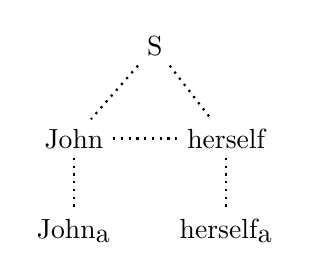
\begin{tikzpicture}[
    every node/.style={align=center},
    dotted line/.style={draw, dotted, thick},
    curved arrow/.style={draw, thick, -{Latex[bend]}},
    ]
\node (S) at (1.532839,0.000000) {S};
\node (John) at (0.505225,-1.171530) {John};
\node (herself) at (2.439394,-1.171530) {herself};
\draw[dotted line] (S) -- (John);
\draw[dotted line] (S) -- (herself);
\draw[dotted line] (John) -- (herself);
\node (JohnA) at (0.505225,-2.343060) {${\textrm{John}_{\textrm{a}}}$};
\node (herselfA) at (2.439394,-2.343060) {${\textrm{herself}_{\textrm{a}}}$};
\draw[dotted line] (John) -- (JohnA);
\draw[dotted line] (herself) -- (herselfA);
\end{tikzpicture}
}
\end{minipage}
\bigbreak

\clearpage

%%%%%%%%%%%%%%%%%%%%%%%%%%%%%%%%%%%%%%%%%%%%%%%%%%%%%%%%%%%%%%%%
%
%     (1.4) Some students think they are smarter than they are.
%
%%%%%%%%%%%%%%%%%%%%%%%%%%%%%%%%%%%%%%%%%%%%%%%%%%%%%%%%%%%%%%%%

\section*{(1.4) Some students think they are smarter than they are.}
\addcontentsline{toc}{section}{(1.4) Some students think they are smarter than they are.}

\bigbreak
\begin{enumerate*}
\item[(1.4)] Some students think they are smarter than they are.
\end{enumerate*}
\bigbreak

\bigbreak
\begin{minipage}{\textwidth}
\makebox[\textwidth][c]{
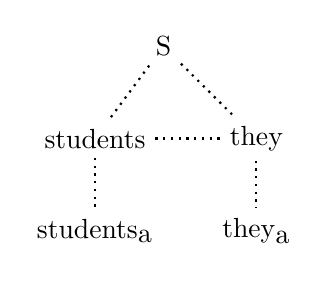
\begin{tikzpicture}[
    every node/.style={align=center},
    dotted line/.style={draw, dotted, thick},
    curved arrow/.style={draw, thick, -{Latex[bend]}},
    ]
\node (S) at (1.648040,0.000000) {S};
\node (students) at (0.778095,-1.171530) {students};
\node (they) at (2.827465,-1.171530) {they};
\draw[dotted line] (S) -- (students);
\draw[dotted line] (S) -- (they);
\draw[dotted line] (students) -- (they);
\node (studentsA) at (0.778095,-2.343060) {${\textrm{students}_{\textrm{a}}}$};
\node (theyA) at (2.827465,-2.343060) {${\textrm{they}_{\textrm{a}}}$};
\draw[dotted line] (students) -- (studentsA);
\draw[dotted line] (they) -- (theyA);
\end{tikzpicture}
}
\end{minipage}
\bigbreak

\clearpage

%%%%%%%%%%%%%%%%%%%%%%%%%%%%%%%%%%%%%%%%%%%%%%%%%%%%%%%%%%%%%%%%
%
%     (1.6) My uncle has never ridden a camel but his brother has, although it was lame.
%
%%%%%%%%%%%%%%%%%%%%%%%%%%%%%%%%%%%%%%%%%%%%%%%%%%%%%%%%%%%%%%%%

\section*{(1.6) My uncle has never ridden a camel but his brother has, although it was lame.}
\addcontentsline{toc}{section}{(1.6) My uncle has never ridden a camel but his brother has, although it was lame.}

\bigbreak
\begin{enumerate*}
\item[(1.6)] My uncle has never ridden a camel but his brother has, although it was lame.
\end{enumerate*}
\bigbreak

\bigbreak
\begin{minipage}{\textwidth}
\makebox[\textwidth][c]{
\begin{tikzpicture}[
    every node/.style={align=center},
    dotted line/.style={draw, dotted, thick},
    curved arrow/.style={draw, thick, -{Latex[bend]}},
    ]
\node (S) at (4.776359,0.000000) {S};
\node (my) at (0.370987,-1.171530) {my};
\node (uncle) at (2.076707,-1.171530) {uncle};
\node (camel) at (3.982564,-1.171530) {camel};
\node (his) at (5.703904,-1.171530) {his};
\node (brother) at (7.553137,-1.171530) {brother};
\node (it) at (9.303766,-1.171530) {it};
\draw[dotted line] (S) -- (my);
\draw[dotted line] (S) -- (it);
\draw[dotted line] (my) -- (uncle);
\draw[dotted line] (uncle) -- (camel);
\draw[dotted line] (camel) -- (his);
\draw[dotted line] (his) -- (brother);
\draw[dotted line] (brother) -- (it);
\node (myA) at (0.370987,-2.343060) {${\textrm{my}_{\textrm{a}}}$};
\node (uncleA) at (2.076707,-2.343060) {${\textrm{uncle}_{\textrm{a}}}$};
\node (camelA) at (3.982564,-2.343060) {${\textrm{camel}_{\textrm{a}}}$};
\node (hisA) at (5.703904,-2.343060) {${\textrm{his}_{\textrm{a}}}$};
\node (brotherA) at (7.553137,-2.343060) {${\textrm{brother}_{\textrm{a}}}$};
\node (itA) at (9.303766,-2.343060) {${\textrm{it}_{\textrm{a}}}$};
\draw[dotted line] (my) -- (myA);
\draw[dotted line] (uncle) -- (uncleA);
\draw[dotted line] (camel) -- (camelA);
\draw[dotted line] (his) -- (hisA);
\draw[dotted line] (brother) -- (brotherA);
\draw[dotted line] (it) -- (itA);
\node (uncleB) at (2.076707,-3.514590) {${\textrm{uncle}_{\textrm{b}}}$};
\node (camelB) at (3.982564,-3.514590) {${\textrm{camel}_{\textrm{b}}}$};
\draw[dotted line] (uncleA) -- (uncleB);
\draw[dotted line] (camelA) -- (camelB);
\draw[curved arrow] (camelB.north east) to [out=58.59,in=-81.23] (hisA.south);
\draw[curved arrow] (uncleB.north east) to [out=39.31,in=179.13] (hisA.west);
\end{tikzpicture}
}
\end{minipage}
\bigbreak

\clearpage

%%%%%%%%%%%%%%%%%%%%%%%%%%%%%%%%%%%%%%%%%%%%%%%%%%%%%%%%%%%%%%%%
%
%     (1.10) I like the fresh candy better than the stale PHI.
%
%%%%%%%%%%%%%%%%%%%%%%%%%%%%%%%%%%%%%%%%%%%%%%%%%%%%%%%%%%%%%%%%

\section*{(1.10) I like the fresh candy better than the stale PHI.}
\addcontentsline{toc}{section}{(1.10) I like the fresh candy better than the stale PHI.}

\bigbreak
\begin{enumerate*}
\item[(1.10)] I like the fresh candy better than the stale PHI.
\end{enumerate*}
\bigbreak

\bigbreak
\begin{minipage}{\textwidth}
\makebox[\textwidth][c]{
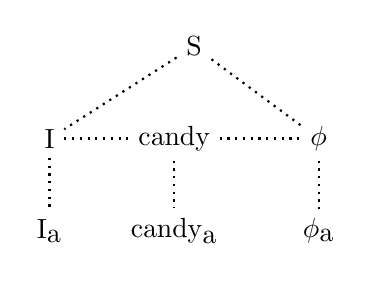
\begin{tikzpicture}[
    every node/.style={align=center},
    dotted line/.style={draw, dotted, thick},
    curved arrow/.style={draw, thick, -{Latex[bend]}},
    ]
\node (S) at (2.030333,0.000000) {S};
\node (I) at (0.195256,-1.171530) {I};
\node (candy) at (1.778941,-1.171530) {candy};
\node (PHI) at (3.614018,-1.171530) {$\phi$};
\draw[dotted line] (S) -- (I);
\draw[dotted line] (S) -- (PHI);
\draw[dotted line] (I) -- (candy);
\draw[dotted line] (candy) -- (PHI);
\node (IA) at (0.195256,-2.343060) {${\textrm{I}_{\textrm{a}}}$};
\node (candyA) at (1.778941,-2.343060) {${\textrm{candy}_{\textrm{a}}}$};
\node (PHIA) at (3.614018,-2.343060) {${\phi_{\textrm{a}}}$};
\draw[dotted line] (I) -- (IA);
\draw[dotted line] (candy) -- (candyA);
\draw[dotted line] (PHI) -- (PHIA);
\end{tikzpicture}
}
\end{minipage}
\bigbreak

\clearpage

%%%%%%%%%%%%%%%%%%%%%%%%%%%%%%%%%%%%%%%%%%%%%%%%%%%%%%%%%%%%%%%%
%
%     (1.11) If John can, he will do it.
%
%%%%%%%%%%%%%%%%%%%%%%%%%%%%%%%%%%%%%%%%%%%%%%%%%%%%%%%%%%%%%%%%

\section*{(1.11) If John can, he will do it.}
\addcontentsline{toc}{section}{(1.11) If John can, he will do it.}

\bigbreak
\begin{enumerate*}
\item[(1.11)] If John can, he will do it.
\end{enumerate*}
\bigbreak

\bigbreak
\begin{minipage}{\textwidth}
\makebox[\textwidth][c]{
\begin{tikzpicture}[
    every node/.style={align=center},
    dotted line/.style={draw, dotted, thick},
    curved arrow/.style={draw, thick, -{Latex[bend]}},
    ]
\node (S) at (1.214084,0.000000) {S};
\node (John) at (0.505225,-1.171530) {John};
\node (he) at (2.120639,-1.171530) {he};
\draw[dotted line] (S) -- (John);
\draw[dotted line] (S) -- (he);
\draw[dotted line] (John) -- (he);
\node (JohnA) at (0.505225,-2.343060) {${\textrm{John}_{\textrm{a}}}$};
\node (heA) at (2.120639,-2.343060) {${\textrm{he}_{\textrm{a}}}$};
\draw[dotted line] (John) -- (JohnA);
\draw[dotted line] (he) -- (heA);
\node (JohnB) at (0.505225,-3.514590) {${\textrm{John}_{\textrm{b}}}$};
\draw[dotted line] (JohnA) -- (JohnB);
\draw[curved arrow] (JohnB.north east) to [out=58.59,in=-121.41] (heA.south west);
\end{tikzpicture}
}
\end{minipage}
\bigbreak

\clearpage

%%%%%%%%%%%%%%%%%%%%%%%%%%%%%%%%%%%%%%%%%%%%%%%%%%%%%%%%%%%%%%%%
%
%     (1.12) If he can, John will do it.
%
%%%%%%%%%%%%%%%%%%%%%%%%%%%%%%%%%%%%%%%%%%%%%%%%%%%%%%%%%%%%%%%%

\section*{(1.12) If he can, John will do it.}
\addcontentsline{toc}{section}{(1.12) If he can, John will do it.}

\bigbreak
\begin{enumerate*}
\item[(1.12)] If he can, John will do it.
\end{enumerate*}
\bigbreak

\bigbreak
\begin{minipage}{\textwidth}
\makebox[\textwidth][c]{
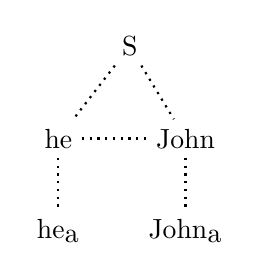
\begin{tikzpicture}[
    every node/.style={align=center},
    dotted line/.style={draw, dotted, thick},
    curved arrow/.style={draw, thick, -{Latex[bend]}},
    ]
\node (S) at (1.214084,0.000000) {S};
\node (he) at (0.307528,-1.171530) {he};
\node (John) at (1.922942,-1.171530) {John};
\draw[dotted line] (S) -- (he);
\draw[dotted line] (S) -- (John);
\draw[dotted line] (he) -- (John);
\node (heA) at (0.307528,-2.343060) {${\textrm{he}_{\textrm{a}}}$};
\node (JohnA) at (1.922942,-2.343060) {${\textrm{John}_{\textrm{a}}}$};
\draw[dotted line] (he) -- (heA);
\draw[dotted line] (John) -- (JohnA);
\end{tikzpicture}
}
\end{minipage}
\bigbreak

\clearpage

%%%%%%%%%%%%%%%%%%%%%%%%%%%%%%%%%%%%%%%%%%%%%%%%%%%%%%%%%%%%%%%%
%
%     (1.13) John will do it if he can.
%
%%%%%%%%%%%%%%%%%%%%%%%%%%%%%%%%%%%%%%%%%%%%%%%%%%%%%%%%%%%%%%%%

\section*{(1.13) John will do it if he can.}
\addcontentsline{toc}{section}{(1.13) John will do it if he can.}

\bigbreak
\begin{enumerate*}
\item[(1.13)] John will do it if he can.
\end{enumerate*}
\bigbreak

\bigbreak
\begin{minipage}{\textwidth}
\makebox[\textwidth][c]{
\begin{tikzpicture}[
    every node/.style={align=center},
    dotted line/.style={draw, dotted, thick},
    curved arrow/.style={draw, thick, -{Latex[bend]}},
    ]
\node (S) at (1.214084,0.000000) {S};
\node (John) at (0.505225,-1.171530) {John};
\node (he) at (2.120639,-1.171530) {he};
\draw[dotted line] (S) -- (John);
\draw[dotted line] (S) -- (he);
\draw[dotted line] (John) -- (he);
\node (JohnA) at (0.505225,-2.343060) {${\textrm{John}_{\textrm{a}}}$};
\node (heA) at (2.120639,-2.343060) {${\textrm{he}_{\textrm{a}}}$};
\draw[dotted line] (John) -- (JohnA);
\draw[dotted line] (he) -- (heA);
\node (JohnB) at (0.505225,-3.514590) {${\textrm{John}_{\textrm{b}}}$};
\draw[dotted line] (JohnA) -- (JohnB);
\draw[curved arrow] (JohnB.north east) to [out=58.59,in=-121.41] (heA.south west);
\end{tikzpicture}
}
\end{minipage}
\bigbreak

\clearpage

%%%%%%%%%%%%%%%%%%%%%%%%%%%%%%%%%%%%%%%%%%%%%%%%%%%%%%%%%%%%%%%%
%
%     (1.14) He will do it if John can.
%
%%%%%%%%%%%%%%%%%%%%%%%%%%%%%%%%%%%%%%%%%%%%%%%%%%%%%%%%%%%%%%%%

\section*{(1.14) He will do it if John can.}
\addcontentsline{toc}{section}{(1.14) He will do it if John can.}

\bigbreak
\begin{enumerate*}
\item[(1.14)] He will do it if John can.
\end{enumerate*}
\bigbreak

\bigbreak
\begin{minipage}{\textwidth}
\makebox[\textwidth][c]{
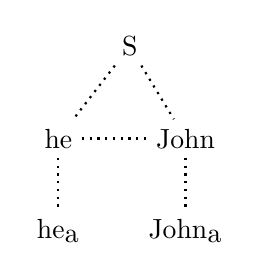
\begin{tikzpicture}[
    every node/.style={align=center},
    dotted line/.style={draw, dotted, thick},
    curved arrow/.style={draw, thick, -{Latex[bend]}},
    ]
\node (S) at (1.214084,0.000000) {S};
\node (he) at (0.307528,-1.171530) {he};
\node (John) at (1.922942,-1.171530) {John};
\draw[dotted line] (S) -- (he);
\draw[dotted line] (S) -- (John);
\draw[dotted line] (he) -- (John);
\node (heA) at (0.307528,-2.343060) {${\textrm{he}_{\textrm{a}}}$};
\node (JohnA) at (1.922942,-2.343060) {${\textrm{John}_{\textrm{a}}}$};
\draw[dotted line] (he) -- (heA);
\draw[dotted line] (John) -- (JohnA);
\end{tikzpicture}
}
\end{minipage}
\bigbreak

\clearpage

%%%%%%%%%%%%%%%%%%%%%%%%%%%%%%%%%%%%%%%%%%%%%%%%%%%%%%%%%%%%%%%%
%
%     (1.24) I have a cat at home, but hate it.
%
%%%%%%%%%%%%%%%%%%%%%%%%%%%%%%%%%%%%%%%%%%%%%%%%%%%%%%%%%%%%%%%%

\section*{(1.24) I have a cat at home, but hate it.}
\addcontentsline{toc}{section}{(1.24) I have a cat at home, but hate it.}

\bigbreak
\begin{enumerate*}
\item[(1.24)] I have a cat at home, but hate it.
\end{enumerate*}
\bigbreak

\bigbreak
\begin{minipage}{\textwidth}
\makebox[\textwidth][c]{
\begin{tikzpicture}[
    every node/.style={align=center},
    dotted line/.style={draw, dotted, thick},
    curved arrow/.style={draw, thick, -{Latex[bend]}},
    ]
\node (S) at (3.404118,0.000000) {S};
\node (I) at (0.195256,-1.171530) {I};
\node (cat) at (1.559278,-1.171530) {cat};
\node (home) at (3.269879,-1.171530) {home};
\node (PHI) at (5.061024,-1.171530) {$\phi$};
\node (it) at (6.559284,-1.171530) {it};
\draw[dotted line] (S) -- (I);
\draw[dotted line] (S) -- (it);
\draw[dotted line] (I) -- (cat);
\draw[dotted line] (cat) -- (home);
\draw[dotted line] (home) -- (PHI);
\draw[dotted line] (PHI) -- (it);
\node (IA) at (0.195256,-2.343060) {${\textrm{I}_{\textrm{a}}}$};
\node (catA) at (1.559278,-2.343060) {${\textrm{cat}_{\textrm{a}}}$};
\node (homeA) at (3.269879,-2.343060) {${\textrm{home}_{\textrm{a}}}$};
\node (PHIA) at (5.061024,-2.343060) {${\phi_{\textrm{a}}}$};
\node (itA) at (6.559284,-2.343060) {${\textrm{it}_{\textrm{a}}}$};
\draw[dotted line] (I) -- (IA);
\draw[dotted line] (cat) -- (catA);
\draw[dotted line] (home) -- (homeA);
\draw[dotted line] (PHI) -- (PHIA);
\draw[dotted line] (it) -- (itA);
\node (IB) at (0.195256,-3.514590) {${\textrm{I}_{\textrm{b}}}$};
\node (catB) at (1.559278,-3.514590) {${\textrm{cat}_{\textrm{b}}}$};
\node (homeB) at (3.269879,-3.514590) {${\textrm{home}_{\textrm{b}}}$};
\draw[dotted line] (IA) -- (IB);
\draw[dotted line] (catA) -- (catB);
\draw[dotted line] (homeA) -- (homeB);
\node (homeC) at (3.269879,-4.686120) {${\textrm{home}_{\textrm{c}}}$};
\draw[dotted line] (homeB) -- (homeC);
\draw[curved arrow] (homeC.north) to [out=73.02,in=-73.41] (PHIA.south);
\draw[curved arrow] (catB.north east) to [out=39.31,in=-150.27] (PHIA.south west);
\draw[curved arrow] (IB.north east) to [out=28.62,in=144.39] (PHIA.north west);
\draw[curved arrow] (homeB.north east) to [out=39.31,in=-140.69] (itA.south west);
\end{tikzpicture}
}
\end{minipage}
\bigbreak

\clearpage

%%%%%%%%%%%%%%%%%%%%%%%%%%%%%%%%%%%%%%%%%%%%%%%%%%%%%%%%%%%%%%%%
%
%     (1.25) I want to get a cat for myself.
%
%%%%%%%%%%%%%%%%%%%%%%%%%%%%%%%%%%%%%%%%%%%%%%%%%%%%%%%%%%%%%%%%

\section*{(1.25) I want to get a cat for myself.}
\addcontentsline{toc}{section}{(1.25) I want to get a cat for myself.}

\bigbreak
\begin{enumerate*}
\item[(1.25)] I want to get a cat for myself.
\end{enumerate*}
\bigbreak

\bigbreak
\begin{minipage}{\textwidth}
\makebox[\textwidth][c]{
\begin{tikzpicture}[
    every node/.style={align=center},
    dotted line/.style={draw, dotted, thick},
    curved arrow/.style={draw, thick, -{Latex[bend]}},
    ]
\node (S) at (2.832915,0.000000) {S};
\node (I) at (0.195256,-1.171530) {I};
\node (PHI) at (1.639821,-1.171530) {$\phi$};
\node (cat) at (3.255235,-1.171530) {cat};
\node (myself) at (5.044915,-1.171530) {myself};
\draw[dotted line] (S) -- (I);
\draw[dotted line] (S) -- (myself);
\draw[dotted line] (I) -- (PHI);
\draw[dotted line] (PHI) -- (cat);
\draw[dotted line] (cat) -- (myself);
\node (IA) at (0.195256,-2.343060) {${\textrm{I}_{\textrm{a}}}$};
\node (PHIA) at (1.639821,-2.343060) {${\phi_{\textrm{a}}}$};
\node (catA) at (3.255235,-2.343060) {${\textrm{cat}_{\textrm{a}}}$};
\node (myselfA) at (5.044915,-2.343060) {${\textrm{myself}_{\textrm{a}}}$};
\draw[dotted line] (I) -- (IA);
\draw[dotted line] (PHI) -- (PHIA);
\draw[dotted line] (cat) -- (catA);
\draw[dotted line] (myself) -- (myselfA);
\node (IB) at (0.195256,-3.514590) {${\textrm{I}_{\textrm{b}}}$};
\node (PHIB) at (1.639821,-3.514590) {${\phi_{\textrm{b}}}$};
\draw[dotted line] (IA) -- (IB);
\draw[dotted line] (PHIA) -- (PHIB);
\node (IC) at (0.195256,-4.686120) {${\textrm{I}_{\textrm{c}}}$};
\draw[dotted line] (IB) -- (IC);
\draw[curved arrow] (IB.north east) to [out=58.59,in=-121.41] (PHIA.south west);
\draw[curved arrow] (PHIB.north east) to [out=39.31,in=-140.69] (myselfA.south west);
\draw[curved arrow] (IC.north east) to [out=58.59,in=-121.41] (PHIB.south west);
\end{tikzpicture}
}
\end{minipage}
\bigbreak

\clearpage

%%%%%%%%%%%%%%%%%%%%%%%%%%%%%%%%%%%%%%%%%%%%%%%%%%%%%%%%%%%%%%%%
%
%     (1.27) The men took off their hats.
%
%%%%%%%%%%%%%%%%%%%%%%%%%%%%%%%%%%%%%%%%%%%%%%%%%%%%%%%%%%%%%%%%

\section*{(1.27) The men took off their hats.}
\addcontentsline{toc}{section}{(1.27) The men took off their hats.}

\bigbreak
\begin{enumerate*}
\item[(1.27)] The men took off their hats.
\end{enumerate*}
\bigbreak

\bigbreak
\begin{minipage}{\textwidth}
\makebox[\textwidth][c]{
\begin{tikzpicture}[
    every node/.style={align=center},
    dotted line/.style={draw, dotted, thick},
    curved arrow/.style={draw, thick, -{Latex[bend]}},
    ]
\node (S) at (2.205087,0.000000) {S};
\node (men) at (0.453970,-1.171530) {men};
\node (their) at (2.204111,-1.171530) {their};
\node (hats) at (3.955228,-1.171530) {hats};
\draw[dotted line] (S) -- (men);
\draw[dotted line] (S) -- (hats);
\draw[dotted line] (men) -- (their);
\draw[dotted line] (their) -- (hats);
\node (menA) at (0.453970,-2.343060) {${\textrm{men}_{\textrm{a}}}$};
\node (theirA) at (2.204111,-2.343060) {${\textrm{their}_{\textrm{a}}}$};
\node (hatsA) at (3.955228,-2.343060) {${\textrm{hats}_{\textrm{a}}}$};
\draw[dotted line] (men) -- (menA);
\draw[dotted line] (their) -- (theirA);
\draw[dotted line] (hats) -- (hatsA);
\node (menB) at (0.453970,-3.514590) {${\textrm{men}_{\textrm{b}}}$};
\draw[dotted line] (menA) -- (menB);
\draw[curved arrow] (menB.north east) to [out=58.59,in=-121.41] (theirA.south west);
\end{tikzpicture}
}
\end{minipage}
\bigbreak

\clearpage

%%%%%%%%%%%%%%%%%%%%%%%%%%%%%%%%%%%%%%%%%%%%%%%%%%%%%%%%%%%%%%%%
%
%     (1.51) The man who lives next door said that he would mow my lawn.
%
%%%%%%%%%%%%%%%%%%%%%%%%%%%%%%%%%%%%%%%%%%%%%%%%%%%%%%%%%%%%%%%%

\section*{(1.51) The man who lives next door said that he would mow my lawn.}
\addcontentsline{toc}{section}{(1.51) The man who lives next door said that he would mow my lawn.}

\bigbreak
\begin{enumerate*}
\item[(1.51)] The man who lives next door said that he would mow my lawn.
\end{enumerate*}
\bigbreak

\bigbreak
\begin{minipage}{\textwidth}
\makebox[\textwidth][c]{
\begin{tikzpicture}[
    every node/.style={align=center},
    dotted line/.style={draw, dotted, thick},
    curved arrow/.style={draw, thick, -{Latex[bend]}},
    ]
\node (S) at (2.839261,0.000000) {S};
\node (man) at (0.463733,-1.171530) {man};
\node (he) at (2.037656,-1.171530) {he};
\node (my) at (3.518832,-1.171530) {my};
\node (lawn) at (5.185501,-1.171530) {lawn};
\draw[dotted line] (S) -- (man);
\draw[dotted line] (S) -- (lawn);
\draw[dotted line] (man) -- (he);
\draw[dotted line] (he) -- (my);
\draw[dotted line] (my) -- (lawn);
\node (manA) at (0.463733,-2.343060) {${\textrm{man}_{\textrm{a}}}$};
\node (heA) at (2.037656,-2.343060) {${\textrm{he}_{\textrm{a}}}$};
\node (myA) at (3.518832,-2.343060) {${\textrm{my}_{\textrm{a}}}$};
\node (lawnA) at (5.185501,-2.343060) {${\textrm{lawn}_{\textrm{a}}}$};
\draw[dotted line] (man) -- (manA);
\draw[dotted line] (he) -- (heA);
\draw[dotted line] (my) -- (myA);
\draw[dotted line] (lawn) -- (lawnA);
\node (manB) at (0.463733,-3.514590) {${\textrm{man}_{\textrm{b}}}$};
\draw[dotted line] (manA) -- (manB);
\draw[curved arrow] (manB.north east) to [out=58.59,in=-121.41] (heA.south west);
\end{tikzpicture}
}
\end{minipage}
\bigbreak

\clearpage

%%%%%%%%%%%%%%%%%%%%%%%%%%%%%%%%%%%%%%%%%%%%%%%%%%%%%%%%%%%%%%%%
%
%     (1.52) Somebody seduced Bill's sister, but no one will ever seduce Jack’s and she knows it.
%
%%%%%%%%%%%%%%%%%%%%%%%%%%%%%%%%%%%%%%%%%%%%%%%%%%%%%%%%%%%%%%%%

\section*{(1.52) Somebody seduced Bill's sister, but no one will ever seduce Jack’s and she knows it.}
\addcontentsline{toc}{section}{(1.52) Somebody seduced Bill's sister, but no one will ever seduce Jack’s and she knows it.}

\bigbreak
\begin{enumerate*}
\item[(1.52)] Somebody seduced Bill's sister, but no one will ever seduce Jack’s and she knows it.
\end{enumerate*}
\bigbreak

\bigbreak
\begin{minipage}{\textwidth}
\makebox[\textwidth][c]{
\begin{tikzpicture}[
    every node/.style={align=center},
    dotted line/.style={draw, dotted, thick},
    curved arrow/.style={draw, thick, -{Latex[bend]}},
    ]
\node (S) at (5.373842,0.000000) {S};
\node (somebody) at (0.889391,-1.171530) {somebody};
\node (Bill's) at (3.102289,-1.171530) {Bill's};
\node (sister) at (4.960309,-1.171530) {sister};
\node (Jack's) at (6.896430,-1.171530) {Jack's};
\node (PHI) at (8.744687,-1.171530) {$\phi$};
\node (she) at (10.370840,-1.171530) {she};
\draw[dotted line] (S) -- (somebody);
\draw[dotted line] (S) -- (she);
\draw[dotted line] (somebody) -- (Bill's);
\draw[dotted line] (Bill's) -- (sister);
\draw[dotted line] (sister) -- (Jack's);
\draw[dotted line] (Jack's) -- (PHI);
\draw[dotted line] (PHI) -- (she);
\node (somebodyA) at (0.889391,-2.343060) {${\textrm{somebody}_{\textrm{a}}}$};
\node (Bill'sA) at (3.102289,-2.343060) {${\textrm{Bill's}_{\textrm{a}}}$};
\node (sisterA) at (4.960309,-2.343060) {${\textrm{sister}_{\textrm{a}}}$};
\node (Jack'sA) at (6.896430,-2.343060) {${\textrm{Jack's}_{\textrm{a}}}$};
\node (PHIA) at (8.744687,-2.343060) {${\phi_{\textrm{a}}}$};
\node (sheA) at (10.370840,-2.343060) {${\textrm{she}_{\textrm{a}}}$};
\draw[dotted line] (somebody) -- (somebodyA);
\draw[dotted line] (Bill's) -- (Bill'sA);
\draw[dotted line] (sister) -- (sisterA);
\draw[dotted line] (Jack's) -- (Jack'sA);
\draw[dotted line] (PHI) -- (PHIA);
\draw[dotted line] (she) -- (sheA);
\node (somebodyB) at (0.889391,-3.514590) {${\textrm{somebody}_{\textrm{b}}}$};
\node (sisterB) at (4.960309,-3.514590) {${\textrm{sister}_{\textrm{b}}}$};
\node (PHIB) at (8.744687,-3.514590) {${\phi_{\textrm{b}}}$};
\draw[dotted line] (somebodyA) -- (somebodyB);
\draw[dotted line] (sisterA) -- (sisterB);
\draw[dotted line] (PHIA) -- (PHIB);
\node (somebodyC) at (0.889391,-4.686120) {${\textrm{somebody}_{\textrm{c}}}$};
\node (sisterC) at (4.960309,-4.686120) {${\textrm{sister}_{\textrm{c}}}$};
\draw[dotted line] (somebodyB) -- (somebodyC);
\draw[dotted line] (sisterB) -- (sisterC);
\node (somebodyD) at (0.889391,-5.857650) {${\textrm{somebody}_{\textrm{d}}}$};
\node (sisterD) at (4.960309,-5.857650) {${\textrm{sister}_{\textrm{d}}}$};
\draw[dotted line] (somebodyC) -- (somebodyD);
\draw[dotted line] (sisterC) -- (sisterD);
\draw[curved arrow] (PHIB.north east) to [out=58.59,in=-85.94] (sheA.south);
\draw[curved arrow] (sisterB.north east) to [out=28.62,in=-160.92] (sheA.west);
\draw[curved arrow] (somebodyB.east) to [out=18.13,in=133.83] (sheA.north west);
\draw[curved arrow] (sisterC.north east) to [out=58.59,in=-81.23] (PHIA.south);
\draw[curved arrow] (somebodyC.north east) to [out=39.31,in=179.13] (PHIA.west);
\draw[curved arrow] (sisterD.north east) to [out=58.59,in=-81.23] (PHIB.south);
\draw[curved arrow] (somebodyD.north east) to [out=39.31,in=179.13] (PHIB.west);
\end{tikzpicture}
}
\end{minipage}
\bigbreak

\clearpage

%%%%%%%%%%%%%%%%%%%%%%%%%%%%%%%%%%%%%%%%%%%%%%%%%%%%%%%%%%%%%%%%
%
%     (1.66) Realizing that he was unpopular didn't disturb Oscar.
%
%%%%%%%%%%%%%%%%%%%%%%%%%%%%%%%%%%%%%%%%%%%%%%%%%%%%%%%%%%%%%%%%

\section*{(1.66) Realizing that he was unpopular didn't disturb Oscar.}
\addcontentsline{toc}{section}{(1.66) Realizing that he was unpopular didn't disturb Oscar.}

\bigbreak
\begin{enumerate*}
\item[(1.66)] Realizing that he was unpopular didn't disturb Oscar.
\end{enumerate*}
\bigbreak

\bigbreak
\begin{minipage}{\textwidth}
\makebox[\textwidth][c]{
\begin{tikzpicture}[
    every node/.style={align=center},
    dotted line/.style={draw, dotted, thick},
    curved arrow/.style={draw, thick, -{Latex[bend]}},
    ]
\node (S) at (2.129425,0.000000) {S};
\node (PHI) at (0.446648,-1.171530) {$\phi$};
\node (he) at (2.003485,-1.171530) {he};
\node (Oscar) at (3.686262,-1.171530) {Oscar};
\draw[dotted line] (S) -- (PHI);
\draw[dotted line] (S) -- (Oscar);
\draw[dotted line] (PHI) -- (he);
\draw[dotted line] (he) -- (Oscar);
\node (PHIA) at (0.446648,-2.343060) {${\phi_{\textrm{a}}}$};
\node (heA) at (2.003485,-2.343060) {${\textrm{he}_{\textrm{a}}}$};
\node (OscarA) at (3.686262,-2.343060) {${\textrm{Oscar}_{\textrm{a}}}$};
\draw[dotted line] (PHI) -- (PHIA);
\draw[dotted line] (he) -- (heA);
\draw[dotted line] (Oscar) -- (OscarA);
\node (PHIB) at (0.446648,-3.514590) {${\phi_{\textrm{b}}}$};
\node (OscarB) at (3.686262,-3.514590) {${\textrm{Oscar}_{\textrm{b}}}$};
\draw[dotted line] (PHIA) -- (PHIB);
\draw[dotted line] (OscarA) -- (OscarB);
\node (OscarC) at (3.686262,-4.686120) {${\textrm{Oscar}_{\textrm{c}}}$};
\draw[dotted line] (OscarB) -- (OscarC);
\node (OscarD) at (3.686262,-5.857650) {${\textrm{Oscar}_{\textrm{d}}}$};
\draw[dotted line] (OscarC) -- (OscarD);
\draw[curved arrow] (OscarB.north west) to [out=121.41,in=-29.29] (heA.south east);
\draw[curved arrow] (PHIB.north east) to [out=58.59,in=-150.71] (heA.south west);
\draw[curved arrow] (OscarC.north west) to [out=121.41,in=-58.59] (PHIA.south east);
\draw[curved arrow] (OscarD.north west) to [out=121.41,in=-58.59] (PHIB.south east);
\end{tikzpicture}
}
\end{minipage}
\bigbreak

\clearpage

%%%%%%%%%%%%%%%%%%%%%%%%%%%%%%%%%%%%%%%%%%%%%%%%%%%%%%%%%%%%%%%%
%
%     (1.70) My neighbor who is pregnant said that she was very happy.
%
%%%%%%%%%%%%%%%%%%%%%%%%%%%%%%%%%%%%%%%%%%%%%%%%%%%%%%%%%%%%%%%%

\section*{(1.70) My neighbor who is pregnant said that she was very happy.}
\addcontentsline{toc}{section}{(1.70) My neighbor who is pregnant said that she was very happy.}

\bigbreak
\begin{enumerate*}
\item[(1.70)] My neighbor who is pregnant said that she was very happy.
\end{enumerate*}
\bigbreak

\bigbreak
\begin{minipage}{\textwidth}
\makebox[\textwidth][c]{
\begin{tikzpicture}[
    every node/.style={align=center},
    dotted line/.style={draw, dotted, thick},
    curved arrow/.style={draw, thick, -{Latex[bend]}},
    ]
\node (S) at (2.346648,0.000000) {S};
\node (my) at (0.370987,-1.171530) {my};
\node (neighbor) at (2.340791,-1.171530) {neighbor};
\node (she) at (4.316452,-1.171530) {she};
\draw[dotted line] (S) -- (my);
\draw[dotted line] (S) -- (she);
\draw[dotted line] (my) -- (neighbor);
\draw[dotted line] (neighbor) -- (she);
\node (myA) at (0.370987,-2.343060) {${\textrm{my}_{\textrm{a}}}$};
\node (neighborA) at (2.340791,-2.343060) {${\textrm{neighbor}_{\textrm{a}}}$};
\node (sheA) at (4.316452,-2.343060) {${\textrm{she}_{\textrm{a}}}$};
\draw[dotted line] (my) -- (myA);
\draw[dotted line] (neighbor) -- (neighborA);
\draw[dotted line] (she) -- (sheA);
\node (neighborB) at (2.340791,-3.514590) {${\textrm{neighbor}_{\textrm{b}}}$};
\draw[dotted line] (neighborA) -- (neighborB);
\draw[curved arrow] (neighborB.north east) to [out=58.59,in=-121.41] (sheA.south west);
\end{tikzpicture}
}
\end{minipage}
\bigbreak

\clearpage

%%%%%%%%%%%%%%%%%%%%%%%%%%%%%%%%%%%%%%%%%%%%%%%%%%%%%%%%%%%%%%%%
%
%     (1.74) The pilot who shot at it hit the Mig that chased him.
%
%%%%%%%%%%%%%%%%%%%%%%%%%%%%%%%%%%%%%%%%%%%%%%%%%%%%%%%%%%%%%%%%

\section*{(1.74) The pilot who shot at it hit the Mig that chased him.}
\addcontentsline{toc}{section}{(1.74) The pilot who shot at it hit the Mig that chased him.}

\bigbreak
\begin{enumerate*}
\item[(1.74)] The pilot who shot at it hit the Mig that chased him.
\end{enumerate*}
\bigbreak

\bigbreak
\begin{minipage}{\textwidth}
\makebox[\textwidth][c]{
\begin{tikzpicture}[
    every node/.style={align=center},
    dotted line/.style={draw, dotted, thick},
    curved arrow/.style={draw, thick, -{Latex[bend]}},
    ]
\node (S) at (2.790448,0.000000) {S};
\node (pilot) at (0.483259,-1.171530) {pilot};
\node (it) at (2.018131,-1.171530) {it};
\node (Mig) at (3.499307,-1.171530) {Mig};
\node (him) at (5.156214,-1.171530) {him};
\draw[dotted line] (S) -- (pilot);
\draw[dotted line] (S) -- (him);
\draw[dotted line] (pilot) -- (it);
\draw[dotted line] (it) -- (Mig);
\draw[dotted line] (Mig) -- (him);
\node (pilotA) at (0.483259,-2.343060) {${\textrm{pilot}_{\textrm{a}}}$};
\node (itA) at (2.018131,-2.343060) {${\textrm{it}_{\textrm{a}}}$};
\node (MigA) at (3.499307,-2.343060) {${\textrm{Mig}_{\textrm{a}}}$};
\node (himA) at (5.156214,-2.343060) {${\textrm{him}_{\textrm{a}}}$};
\draw[dotted line] (pilot) -- (pilotA);
\draw[dotted line] (it) -- (itA);
\draw[dotted line] (Mig) -- (MigA);
\draw[dotted line] (him) -- (himA);
\node (pilotB) at (0.483259,-3.514590) {${\textrm{pilot}_{\textrm{b}}}$};
\node (MigB) at (3.499307,-3.514590) {${\textrm{Mig}_{\textrm{b}}}$};
\draw[dotted line] (pilotA) -- (pilotB);
\draw[dotted line] (MigA) -- (MigB);
\draw[curved arrow] (pilotB.north east) to [out=28.62,in=-151.38] (himA.south west);
\draw[curved arrow] (MigB.north west) to [out=121.41,in=-58.59] (itA.south east);
\end{tikzpicture}
}
\end{minipage}
\bigbreak

\clearpage

%%%%%%%%%%%%%%%%%%%%%%%%%%%%%%%%%%%%%%%%%%%%%%%%%%%%%%%%%%%%%%%%
%
%     (1.86) The mosquito which bit Algernon was killed by him.
%
%%%%%%%%%%%%%%%%%%%%%%%%%%%%%%%%%%%%%%%%%%%%%%%%%%%%%%%%%%%%%%%%

\section*{(1.86) The mosquito which bit Algernon was killed by him.}
\addcontentsline{toc}{section}{(1.86) The mosquito which bit Algernon was killed by him.}

\bigbreak
\begin{enumerate*}
\item[(1.86)] The mosquito which bit Algernon was killed by him.
\end{enumerate*}
\bigbreak

\bigbreak
\begin{minipage}{\textwidth}
\makebox[\textwidth][c]{
\begin{tikzpicture}[
    every node/.style={align=center},
    dotted line/.style={draw, dotted, thick},
    curved arrow/.style={draw, thick, -{Latex[bend]}},
    ]
\node (S) at (2.888484,0.000000) {S};
\node (mosquito) at (0.830815,-1.171530) {mosquito};
\node (Algernon) at (3.294617,-1.171530) {Algernon};
\node (him) at (5.352286,-1.171530) {him};
\draw[dotted line] (S) -- (mosquito);
\draw[dotted line] (S) -- (him);
\draw[dotted line] (mosquito) -- (Algernon);
\draw[dotted line] (Algernon) -- (him);
\node (mosquitoA) at (0.830815,-2.343060) {${\textrm{mosquito}_{\textrm{a}}}$};
\node (AlgernonA) at (3.294617,-2.343060) {${\textrm{Algernon}_{\textrm{a}}}$};
\node (himA) at (5.352286,-2.343060) {${\textrm{him}_{\textrm{a}}}$};
\draw[dotted line] (mosquito) -- (mosquitoA);
\draw[dotted line] (Algernon) -- (AlgernonA);
\draw[dotted line] (him) -- (himA);
\node (AlgernonB) at (3.294617,-3.514590) {${\textrm{Algernon}_{\textrm{b}}}$};
\draw[dotted line] (AlgernonA) -- (AlgernonB);
\draw[curved arrow] (AlgernonB.north east) to [out=58.59,in=-121.41] (himA.south west);
\end{tikzpicture}
}
\end{minipage}
\bigbreak

\clearpage

%%%%%%%%%%%%%%%%%%%%%%%%%%%%%%%%%%%%%%%%%%%%%%%%%%%%%%%%%%%%%%%%
%
%     (1.87) The mosquito which bit him was killed by Algernon.
%
%%%%%%%%%%%%%%%%%%%%%%%%%%%%%%%%%%%%%%%%%%%%%%%%%%%%%%%%%%%%%%%%

\section*{(1.87) The mosquito which bit him was killed by Algernon.}
\addcontentsline{toc}{section}{(1.87) The mosquito which bit him was killed by Algernon.}

\bigbreak
\begin{enumerate*}
\item[(1.87)] The mosquito which bit him was killed by Algernon.
\end{enumerate*}
\bigbreak

\bigbreak
\begin{minipage}{\textwidth}
\makebox[\textwidth][c]{
\begin{tikzpicture}[
    every node/.style={align=center},
    dotted line/.style={draw, dotted, thick},
    curved arrow/.style={draw, thick, -{Latex[bend]}},
    ]
\node (S) at (2.888484,0.000000) {S};
\node (mosquito) at (0.830815,-1.171530) {mosquito};
\node (him) at (2.888973,-1.171530) {him};
\node (Algernon) at (4.946642,-1.171530) {Algernon};
\draw[dotted line] (S) -- (mosquito);
\draw[dotted line] (S) -- (Algernon);
\draw[dotted line] (mosquito) -- (him);
\draw[dotted line] (him) -- (Algernon);
\node (mosquitoA) at (0.830815,-2.343060) {${\textrm{mosquito}_{\textrm{a}}}$};
\node (himA) at (2.888973,-2.343060) {${\textrm{him}_{\textrm{a}}}$};
\node (AlgernonA) at (4.946642,-2.343060) {${\textrm{Algernon}_{\textrm{a}}}$};
\draw[dotted line] (mosquito) -- (mosquitoA);
\draw[dotted line] (him) -- (himA);
\draw[dotted line] (Algernon) -- (AlgernonA);
\node (mosquitoB) at (0.830815,-3.514590) {${\textrm{mosquito}_{\textrm{b}}}$};
\node (AlgernonB) at (4.946642,-3.514590) {${\textrm{Algernon}_{\textrm{b}}}$};
\draw[dotted line] (mosquitoA) -- (mosquitoB);
\draw[dotted line] (AlgernonA) -- (AlgernonB);
\draw[curved arrow] (AlgernonB.north west) to [out=121.41,in=-29.29] (himA.south east);
\draw[curved arrow] (mosquitoB.north east) to [out=58.59,in=-150.71] (himA.south west);
\end{tikzpicture}
}
\end{minipage}
\bigbreak

\clearpage

%%%%%%%%%%%%%%%%%%%%%%%%%%%%%%%%%%%%%%%%%%%%%%%%%%%%%%%%%%%%%%%%
%
%     (1.88) Algernon killed the mosquito which bit him.
%
%%%%%%%%%%%%%%%%%%%%%%%%%%%%%%%%%%%%%%%%%%%%%%%%%%%%%%%%%%%%%%%%

\section*{(1.88) Algernon killed the mosquito which bit him.}
\addcontentsline{toc}{section}{(1.88) Algernon killed the mosquito which bit him.}

\bigbreak
\begin{enumerate*}
\item[(1.88)] Algernon killed the mosquito which bit him.
\end{enumerate*}
\bigbreak

\bigbreak
\begin{minipage}{\textwidth}
\makebox[\textwidth][c]{
\begin{tikzpicture}[
    every node/.style={align=center},
    dotted line/.style={draw, dotted, thick},
    curved arrow/.style={draw, thick, -{Latex[bend]}},
    ]
\node (S) at (2.888484,0.000000) {S};
\node (Algernon) at (0.830326,-1.171530) {Algernon};
\node (mosquito) at (3.294128,-1.171530) {mosquito};
\node (him) at (5.352286,-1.171530) {him};
\draw[dotted line] (S) -- (Algernon);
\draw[dotted line] (S) -- (him);
\draw[dotted line] (Algernon) -- (mosquito);
\draw[dotted line] (mosquito) -- (him);
\node (AlgernonA) at (0.830326,-2.343060) {${\textrm{Algernon}_{\textrm{a}}}$};
\node (mosquitoA) at (3.294128,-2.343060) {${\textrm{mosquito}_{\textrm{a}}}$};
\node (himA) at (5.352286,-2.343060) {${\textrm{him}_{\textrm{a}}}$};
\draw[dotted line] (Algernon) -- (AlgernonA);
\draw[dotted line] (mosquito) -- (mosquitoA);
\draw[dotted line] (him) -- (himA);
\node (AlgernonB) at (0.830326,-3.514590) {${\textrm{Algernon}_{\textrm{b}}}$};
\node (mosquitoB) at (3.294128,-3.514590) {${\textrm{mosquito}_{\textrm{b}}}$};
\draw[dotted line] (AlgernonA) -- (AlgernonB);
\draw[dotted line] (mosquitoA) -- (mosquitoB);
\draw[curved arrow] (mosquitoB.north east) to [out=58.59,in=-81.23] (himA.south);
\draw[curved arrow] (AlgernonB.north east) to [out=39.31,in=179.13] (himA.west);
\end{tikzpicture}
}
\end{minipage}
\bigbreak

\clearpage

%%%%%%%%%%%%%%%%%%%%%%%%%%%%%%%%%%%%%%%%%%%%%%%%%%%%%%%%%%%%%%%%
%
%     (1.89) He killed the mosquito which bit Algernon.
%
%%%%%%%%%%%%%%%%%%%%%%%%%%%%%%%%%%%%%%%%%%%%%%%%%%%%%%%%%%%%%%%%

\section*{(1.89) He killed the mosquito which bit Algernon.}
\addcontentsline{toc}{section}{(1.89) He killed the mosquito which bit Algernon.}

\bigbreak
\begin{enumerate*}
\item[(1.89)] He killed the mosquito which bit Algernon.
\end{enumerate*}
\bigbreak

\bigbreak
\begin{minipage}{\textwidth}
\makebox[\textwidth][c]{
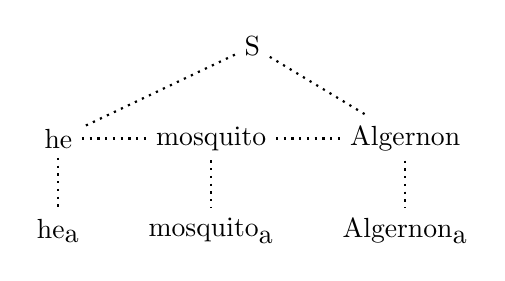
\begin{tikzpicture}[
    every node/.style={align=center},
    dotted line/.style={draw, dotted, thick},
    curved arrow/.style={draw, thick, -{Latex[bend]}},
    ]
\node (S) at (2.771330,0.000000) {S};
\node (he) at (0.307528,-1.171530) {he};
\node (mosquito) at (2.248532,-1.171530) {mosquito};
\node (Algernon) at (4.712334,-1.171530) {Algernon};
\draw[dotted line] (S) -- (he);
\draw[dotted line] (S) -- (Algernon);
\draw[dotted line] (he) -- (mosquito);
\draw[dotted line] (mosquito) -- (Algernon);
\node (heA) at (0.307528,-2.343060) {${\textrm{he}_{\textrm{a}}}$};
\node (mosquitoA) at (2.248532,-2.343060) {${\textrm{mosquito}_{\textrm{a}}}$};
\node (AlgernonA) at (4.712334,-2.343060) {${\textrm{Algernon}_{\textrm{a}}}$};
\draw[dotted line] (he) -- (heA);
\draw[dotted line] (mosquito) -- (mosquitoA);
\draw[dotted line] (Algernon) -- (AlgernonA);
\end{tikzpicture}
}
\end{minipage}
\bigbreak

\clearpage

%%%%%%%%%%%%%%%%%%%%%%%%%%%%%%%%%%%%%%%%%%%%%%%%%%%%%%%%%%%%%%%%
%
%     (1.91) After John Adams woke up, he was hungry.
%
%%%%%%%%%%%%%%%%%%%%%%%%%%%%%%%%%%%%%%%%%%%%%%%%%%%%%%%%%%%%%%%%

\section*{(1.91) After John Adams woke up, he was hungry.}
\addcontentsline{toc}{section}{(1.91) After John Adams woke up, he was hungry.}

\bigbreak
\begin{enumerate*}
\item[(1.91)] After John Adams woke up, he was hungry.
\end{enumerate*}
\bigbreak

\bigbreak
\begin{minipage}{\textwidth}
\makebox[\textwidth][c]{
\begin{tikzpicture}[
    every node/.style={align=center},
    dotted line/.style={draw, dotted, thick},
    curved arrow/.style={draw, thick, -{Latex[bend]}},
    ]
\node (S) at (1.214084,0.000000) {S};
\node (John) at (0.505225,-1.171530) {John};
\node (he) at (2.120639,-1.171530) {he};
\draw[dotted line] (S) -- (John);
\draw[dotted line] (S) -- (he);
\draw[dotted line] (John) -- (he);
\node (JohnA) at (0.505225,-2.343060) {${\textrm{John}_{\textrm{a}}}$};
\node (heA) at (2.120639,-2.343060) {${\textrm{he}_{\textrm{a}}}$};
\draw[dotted line] (John) -- (JohnA);
\draw[dotted line] (he) -- (heA);
\node (JohnB) at (0.505225,-3.514590) {${\textrm{John}_{\textrm{b}}}$};
\draw[dotted line] (JohnA) -- (JohnB);
\draw[curved arrow] (JohnB.north east) to [out=58.59,in=-121.41] (heA.south west);
\end{tikzpicture}
}
\end{minipage}
\bigbreak

\clearpage

%%%%%%%%%%%%%%%%%%%%%%%%%%%%%%%%%%%%%%%%%%%%%%%%%%%%%%%%%%%%%%%%
%
%     (1.92) That Oscar was unpopular didn't disturb him.
%
%%%%%%%%%%%%%%%%%%%%%%%%%%%%%%%%%%%%%%%%%%%%%%%%%%%%%%%%%%%%%%%%

\section*{(1.92) That Oscar was unpopular didn't disturb him.}
\addcontentsline{toc}{section}{(1.92) That Oscar was unpopular didn't disturb him.}

\bigbreak
\begin{enumerate*}
\item[(1.92)] That Oscar was unpopular didn't disturb him.
\end{enumerate*}
\bigbreak

\bigbreak
\begin{minipage}{\textwidth}
\makebox[\textwidth][c]{
\begin{tikzpicture}[
    every node/.style={align=center},
    dotted line/.style={draw, dotted, thick},
    curved arrow/.style={draw, thick, -{Latex[bend]}},
    ]
\node (S) at (1.398601,0.000000) {S};
\node (Oscar) at (0.572588,-1.171530) {Oscar};
\node (him) at (2.372519,-1.171530) {him};
\draw[dotted line] (S) -- (Oscar);
\draw[dotted line] (S) -- (him);
\draw[dotted line] (Oscar) -- (him);
\node (OscarA) at (0.572588,-2.343060) {${\textrm{Oscar}_{\textrm{a}}}$};
\node (himA) at (2.372519,-2.343060) {${\textrm{him}_{\textrm{a}}}$};
\draw[dotted line] (Oscar) -- (OscarA);
\draw[dotted line] (him) -- (himA);
\node (OscarB) at (0.572588,-3.514590) {${\textrm{Oscar}_{\textrm{b}}}$};
\draw[dotted line] (OscarA) -- (OscarB);
\draw[curved arrow] (OscarB.north east) to [out=58.59,in=-121.41] (himA.south west);
\end{tikzpicture}
}
\end{minipage}
\bigbreak

\clearpage

%%%%%%%%%%%%%%%%%%%%%%%%%%%%%%%%%%%%%%%%%%%%%%%%%%%%%%%%%%%%%%%%
%
%     (1.93) For your brother to refuse to pay taxes would get him into trouble.
%
%%%%%%%%%%%%%%%%%%%%%%%%%%%%%%%%%%%%%%%%%%%%%%%%%%%%%%%%%%%%%%%%

\section*{(1.93) For your brother to refuse to pay taxes would get him into trouble.}
\addcontentsline{toc}{section}{(1.93) For your brother to refuse to pay taxes would get him into trouble.}

\bigbreak
\begin{enumerate*}
\item[(1.93)] For your brother to refuse to pay taxes would get him into trouble.
\end{enumerate*}
\bigbreak

\bigbreak
\begin{minipage}{\textwidth}
\makebox[\textwidth][c]{
\begin{tikzpicture}[
    every node/.style={align=center},
    dotted line/.style={draw, dotted, thick},
    curved arrow/.style={draw, thick, -{Latex[bend]}},
    ]
\node (S) at (4.333537,0.000000) {S};
\node (your) at (0.478866,-1.171530) {your};
\node (brother) at (2.459409,-1.171530) {brother};
\node (PHI) at (4.407734,-1.171530) {$\phi$};
\node (him) at (6.081725,-1.171530) {him};
\node (trouble) at (7.988071,-1.171530) {trouble};
\draw[dotted line] (S) -- (your);
\draw[dotted line] (S) -- (trouble);
\draw[dotted line] (your) -- (brother);
\draw[dotted line] (brother) -- (PHI);
\draw[dotted line] (PHI) -- (him);
\draw[dotted line] (him) -- (trouble);
\node (yourA) at (0.478866,-2.343060) {${\textrm{your}_{\textrm{a}}}$};
\node (brotherA) at (2.459409,-2.343060) {${\textrm{brother}_{\textrm{a}}}$};
\node (PHIA) at (4.407734,-2.343060) {${\phi_{\textrm{a}}}$};
\node (himA) at (6.081725,-2.343060) {${\textrm{him}_{\textrm{a}}}$};
\node (troubleA) at (7.988071,-2.343060) {${\textrm{trouble}_{\textrm{a}}}$};
\draw[dotted line] (your) -- (yourA);
\draw[dotted line] (brother) -- (brotherA);
\draw[dotted line] (PHI) -- (PHIA);
\draw[dotted line] (him) -- (himA);
\draw[dotted line] (trouble) -- (troubleA);
\node (brotherB) at (2.459409,-3.514590) {${\textrm{brother}_{\textrm{b}}}$};
\node (PHIB) at (4.407734,-3.514590) {${\phi_{\textrm{b}}}$};
\draw[dotted line] (brotherA) -- (brotherB);
\draw[dotted line] (PHIA) -- (PHIB);
\node (brotherC) at (2.459409,-4.686120) {${\textrm{brother}_{\textrm{c}}}$};
\draw[dotted line] (brotherB) -- (brotherC);
\node (brotherD) at (2.459409,-5.857650) {${\textrm{brother}_{\textrm{d}}}$};
\draw[dotted line] (brotherC) -- (brotherD);
\draw[curved arrow] (PHIB.north east) to [out=58.59,in=-81.23] (himA.south);
\draw[curved arrow] (brotherB.north east) to [out=39.31,in=179.13] (himA.west);
\draw[curved arrow] (brotherC.north) to [out=73.02,in=-106.98] (PHIA.south);
\draw[curved arrow] (brotherD.north) to [out=73.02,in=-106.98] (PHIB.south);
\end{tikzpicture}
}
\end{minipage}
\bigbreak

\clearpage

%%%%%%%%%%%%%%%%%%%%%%%%%%%%%%%%%%%%%%%%%%%%%%%%%%%%%%%%%%%%%%%%
%
%     (1.94) Anna's complaining about Peter infuriated him.
%
%%%%%%%%%%%%%%%%%%%%%%%%%%%%%%%%%%%%%%%%%%%%%%%%%%%%%%%%%%%%%%%%

\section*{(1.94) Anna's complaining about Peter infuriated him.}
\addcontentsline{toc}{section}{(1.94) Anna's complaining about Peter infuriated him.}

\bigbreak
\begin{enumerate*}
\item[(1.94)] Anna's complaining about Peter infuriated him.
\end{enumerate*}
\bigbreak

\bigbreak
\begin{minipage}{\textwidth}
\makebox[\textwidth][c]{
\begin{tikzpicture}[
    every node/.style={align=center},
    dotted line/.style={draw, dotted, thick},
    curved arrow/.style={draw, thick, -{Latex[bend]}},
    ]
\node (S) at (3.897549,0.000000) {S};
\node (Anna's) at (0.664847,-1.171530) {Anna's};
\node (complaining) at (3.191619,-1.171530) {complaining};
\node (Peter) at (5.598309,-1.171530) {Peter};
\node (him) at (7.370415,-1.171530) {him};
\draw[dotted line] (S) -- (Anna's);
\draw[dotted line] (S) -- (him);
\draw[dotted line] (Anna's) -- (complaining);
\draw[dotted line] (complaining) -- (Peter);
\draw[dotted line] (Peter) -- (him);
\node (Anna'sA) at (0.664847,-2.343060) {${\textrm{Anna's}_{\textrm{a}}}$};
\node (complainingA) at (3.191619,-2.343060) {${\textrm{complaining}_{\textrm{a}}}$};
\node (PeterA) at (5.598309,-2.343060) {${\textrm{Peter}_{\textrm{a}}}$};
\node (himA) at (7.370415,-2.343060) {${\textrm{him}_{\textrm{a}}}$};
\draw[dotted line] (Anna's) -- (Anna'sA);
\draw[dotted line] (complaining) -- (complainingA);
\draw[dotted line] (Peter) -- (PeterA);
\draw[dotted line] (him) -- (himA);
\node (PeterB) at (5.598309,-3.514590) {${\textrm{Peter}_{\textrm{b}}}$};
\draw[dotted line] (PeterA) -- (PeterB);
\draw[curved arrow] (PeterB.north east) to [out=58.59,in=-121.41] (himA.south west);
\end{tikzpicture}
}
\end{minipage}
\bigbreak

\clearpage

%%%%%%%%%%%%%%%%%%%%%%%%%%%%%%%%%%%%%%%%%%%%%%%%%%%%%%%%%%%%%%%%
%
%     (1.95) The possibility that Fred will be unpopular doesn’t bother him.
%
%%%%%%%%%%%%%%%%%%%%%%%%%%%%%%%%%%%%%%%%%%%%%%%%%%%%%%%%%%%%%%%%

\section*{(1.95) The possibility that Fred will be unpopular doesn’t bother him.}
\addcontentsline{toc}{section}{(1.95) The possibility that Fred will be unpopular doesn’t bother him.}

\bigbreak
\begin{enumerate*}
\item[(1.95)] The possibility that Fred will be unpopular doesn’t bother him.
\end{enumerate*}
\bigbreak

\bigbreak
\begin{minipage}{\textwidth}
\makebox[\textwidth][c]{
\begin{tikzpicture}[
    every node/.style={align=center},
    dotted line/.style={draw, dotted, thick},
    curved arrow/.style={draw, thick, -{Latex[bend]}},
    ]
\node (S) at (2.628305,0.000000) {S};
\node (possibility) at (0.909893,-1.171530) {possibility};
\node (Fred) at (3.113516,-1.171530) {Fred};
\node (him) at (4.831928,-1.171530) {him};
\draw[dotted line] (S) -- (possibility);
\draw[dotted line] (S) -- (him);
\draw[dotted line] (possibility) -- (Fred);
\draw[dotted line] (Fred) -- (him);
\node (possibilityA) at (0.909893,-2.343060) {${\textrm{possibility}_{\textrm{a}}}$};
\node (FredA) at (3.113516,-2.343060) {${\textrm{Fred}_{\textrm{a}}}$};
\node (himA) at (4.831928,-2.343060) {${\textrm{him}_{\textrm{a}}}$};
\draw[dotted line] (possibility) -- (possibilityA);
\draw[dotted line] (Fred) -- (FredA);
\draw[dotted line] (him) -- (himA);
\node (FredB) at (3.113516,-3.514590) {${\textrm{Fred}_{\textrm{b}}}$};
\draw[dotted line] (FredA) -- (FredB);
\draw[curved arrow] (FredB.north east) to [out=58.59,in=-121.41] (himA.south west);
\end{tikzpicture}
}
\end{minipage}
\bigbreak

\clearpage

%%%%%%%%%%%%%%%%%%%%%%%%%%%%%%%%%%%%%%%%%%%%%%%%%%%%%%%%%%%%%%%%
%
%     (1.96) After he woke up, John Adams was hungry.
%
%%%%%%%%%%%%%%%%%%%%%%%%%%%%%%%%%%%%%%%%%%%%%%%%%%%%%%%%%%%%%%%%

\section*{(1.96) After he woke up, John Adams was hungry.}
\addcontentsline{toc}{section}{(1.96) After he woke up, John Adams was hungry.}

\bigbreak
\begin{enumerate*}
\item[(1.96)] After he woke up, John Adams was hungry.
\end{enumerate*}
\bigbreak

\bigbreak
\begin{minipage}{\textwidth}
\makebox[\textwidth][c]{
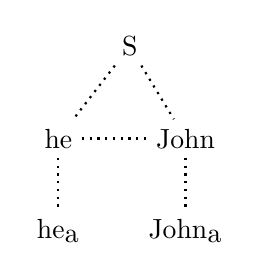
\begin{tikzpicture}[
    every node/.style={align=center},
    dotted line/.style={draw, dotted, thick},
    curved arrow/.style={draw, thick, -{Latex[bend]}},
    ]
\node (S) at (1.214084,0.000000) {S};
\node (he) at (0.307528,-1.171530) {he};
\node (John) at (1.922942,-1.171530) {John};
\draw[dotted line] (S) -- (he);
\draw[dotted line] (S) -- (John);
\draw[dotted line] (he) -- (John);
\node (heA) at (0.307528,-2.343060) {${\textrm{he}_{\textrm{a}}}$};
\node (JohnA) at (1.922942,-2.343060) {${\textrm{John}_{\textrm{a}}}$};
\draw[dotted line] (he) -- (heA);
\draw[dotted line] (John) -- (JohnA);
\end{tikzpicture}
}
\end{minipage}
\bigbreak

\clearpage

%%%%%%%%%%%%%%%%%%%%%%%%%%%%%%%%%%%%%%%%%%%%%%%%%%%%%%%%%%%%%%%%
%
%     (1.97) That he was unpopular didn't disturb Oscar.
%
%%%%%%%%%%%%%%%%%%%%%%%%%%%%%%%%%%%%%%%%%%%%%%%%%%%%%%%%%%%%%%%%

\section*{(1.97) That he was unpopular didn't disturb Oscar.}
\addcontentsline{toc}{section}{(1.97) That he was unpopular didn't disturb Oscar.}

\bigbreak
\begin{enumerate*}
\item[(1.97)] That he was unpopular didn't disturb Oscar.
\end{enumerate*}
\bigbreak

\bigbreak
\begin{minipage}{\textwidth}
\makebox[\textwidth][c]{
\begin{tikzpicture}[
    every node/.style={align=center},
    dotted line/.style={draw, dotted, thick},
    curved arrow/.style={draw, thick, -{Latex[bend]}},
    ]
\node (S) at (1.281446,0.000000) {S};
\node (he) at (0.307528,-1.171530) {he};
\node (Oscar) at (1.990305,-1.171530) {Oscar};
\draw[dotted line] (S) -- (he);
\draw[dotted line] (S) -- (Oscar);
\draw[dotted line] (he) -- (Oscar);
\node (heA) at (0.307528,-2.343060) {${\textrm{he}_{\textrm{a}}}$};
\node (OscarA) at (1.990305,-2.343060) {${\textrm{Oscar}_{\textrm{a}}}$};
\draw[dotted line] (he) -- (heA);
\draw[dotted line] (Oscar) -- (OscarA);
\node (OscarB) at (1.990305,-3.514590) {${\textrm{Oscar}_{\textrm{b}}}$};
\draw[dotted line] (OscarA) -- (OscarB);
\draw[curved arrow] (OscarB.north west) to [out=121.41,in=-58.59] (heA.south east);
\end{tikzpicture}
}
\end{minipage}
\bigbreak

\clearpage

%%%%%%%%%%%%%%%%%%%%%%%%%%%%%%%%%%%%%%%%%%%%%%%%%%%%%%%%%%%%%%%%
%
%     (1.98) For him to refuse to pay taxes would get your brother into trouble.
%
%%%%%%%%%%%%%%%%%%%%%%%%%%%%%%%%%%%%%%%%%%%%%%%%%%%%%%%%%%%%%%%%

\section*{(1.98) For him to refuse to pay taxes would get your brother into trouble.}
\addcontentsline{toc}{section}{(1.98) For him to refuse to pay taxes would get your brother into trouble.}

\bigbreak
\begin{enumerate*}
\item[(1.98)] For him to refuse to pay taxes would get your brother into trouble.
\end{enumerate*}
\bigbreak

\bigbreak
\begin{minipage}{\textwidth}
\makebox[\textwidth][c]{
\begin{tikzpicture}[
    every node/.style={align=center},
    dotted line/.style={draw, dotted, thick},
    curved arrow/.style={draw, thick, -{Latex[bend]}},
    ]
\node (S) at (5.263035,0.000000) {S};
\node (him) at (0.424682,-1.171530) {him};
\node (PHI) at (2.098673,-1.171530) {$\phi$};
\node (taxes) at (3.876150,-1.171530) {taxes};
\node (your) at (5.685844,-1.171530) {your};
\node (brother) at (7.666387,-1.171530) {brother};
\node (trouble) at (9.847067,-1.171530) {trouble};
\draw[dotted line] (S) -- (him);
\draw[dotted line] (S) -- (trouble);
\draw[dotted line] (him) -- (PHI);
\draw[dotted line] (PHI) -- (taxes);
\draw[dotted line] (taxes) -- (your);
\draw[dotted line] (your) -- (brother);
\draw[dotted line] (brother) -- (trouble);
\node (himA) at (0.424682,-2.343060) {${\textrm{him}_{\textrm{a}}}$};
\node (PHIA) at (2.098673,-2.343060) {${\phi_{\textrm{a}}}$};
\node (taxesA) at (3.876150,-2.343060) {${\textrm{taxes}_{\textrm{a}}}$};
\node (yourA) at (5.685844,-2.343060) {${\textrm{your}_{\textrm{a}}}$};
\node (brotherA) at (7.666387,-2.343060) {${\textrm{brother}_{\textrm{a}}}$};
\node (troubleA) at (9.847067,-2.343060) {${\textrm{trouble}_{\textrm{a}}}$};
\draw[dotted line] (him) -- (himA);
\draw[dotted line] (PHI) -- (PHIA);
\draw[dotted line] (taxes) -- (taxesA);
\draw[dotted line] (your) -- (yourA);
\draw[dotted line] (brother) -- (brotherA);
\draw[dotted line] (trouble) -- (troubleA);
\node (himB) at (0.424682,-3.514590) {${\textrm{him}_{\textrm{b}}}$};
\node (PHIB) at (2.098673,-3.514590) {${\phi_{\textrm{b}}}$};
\draw[dotted line] (himA) -- (himB);
\draw[dotted line] (PHIA) -- (PHIB);
\draw[curved arrow] (himB.north east) to [out=58.59,in=-121.41] (PHIA.south west);
\draw[curved arrow] (PHIB.north east) to [out=39.31,in=-140.69] (yourA.south west);
\end{tikzpicture}
}
\end{minipage}
\bigbreak

\clearpage

%%%%%%%%%%%%%%%%%%%%%%%%%%%%%%%%%%%%%%%%%%%%%%%%%%%%%%%%%%%%%%%%
%
%     (1.99) Anna's complaining about him infuriated Peter.
%
%%%%%%%%%%%%%%%%%%%%%%%%%%%%%%%%%%%%%%%%%%%%%%%%%%%%%%%%%%%%%%%%

\section*{(1.99) Anna's complaining about him infuriated Peter.}
\addcontentsline{toc}{section}{(1.99) Anna's complaining about him infuriated Peter.}

\bigbreak
\begin{enumerate*}
\item[(1.99)] Anna's complaining about him infuriated Peter.
\end{enumerate*}
\bigbreak

\bigbreak
\begin{minipage}{\textwidth}
\makebox[\textwidth][c]{
\begin{tikzpicture}[
    every node/.style={align=center},
    dotted line/.style={draw, dotted, thick},
    curved arrow/.style={draw, thick, -{Latex[bend]}},
    ]
\node (S) at (3.897549,0.000000) {S};
\node (Anna's) at (0.664847,-1.171530) {Anna's};
\node (complaining) at (3.191619,-1.171530) {complaining};
\node (him) at (5.478227,-1.171530) {him};
\node (Peter) at (7.250334,-1.171530) {Peter};
\draw[dotted line] (S) -- (Anna's);
\draw[dotted line] (S) -- (Peter);
\draw[dotted line] (Anna's) -- (complaining);
\draw[dotted line] (complaining) -- (him);
\draw[dotted line] (him) -- (Peter);
\node (Anna'sA) at (0.664847,-2.343060) {${\textrm{Anna's}_{\textrm{a}}}$};
\node (complainingA) at (3.191619,-2.343060) {${\textrm{complaining}_{\textrm{a}}}$};
\node (himA) at (5.478227,-2.343060) {${\textrm{him}_{\textrm{a}}}$};
\node (PeterA) at (7.250334,-2.343060) {${\textrm{Peter}_{\textrm{a}}}$};
\draw[dotted line] (Anna's) -- (Anna'sA);
\draw[dotted line] (complaining) -- (complainingA);
\draw[dotted line] (him) -- (himA);
\draw[dotted line] (Peter) -- (PeterA);
\node (PeterB) at (7.250334,-3.514590) {${\textrm{Peter}_{\textrm{b}}}$};
\draw[dotted line] (PeterA) -- (PeterB);
\draw[curved arrow] (PeterB.north west) to [out=121.41,in=-58.59] (himA.south east);
\end{tikzpicture}
}
\end{minipage}
\bigbreak

\clearpage

%%%%%%%%%%%%%%%%%%%%%%%%%%%%%%%%%%%%%%%%%%%%%%%%%%%%%%%%%%%%%%%%
%
%     (1.100) The possibility that he will be unpopular doesn’t bother Fred.
%
%%%%%%%%%%%%%%%%%%%%%%%%%%%%%%%%%%%%%%%%%%%%%%%%%%%%%%%%%%%%%%%%

\section*{(1.100) The possibility that he will be unpopular doesn’t bother Fred.}
\addcontentsline{toc}{section}{(1.100) The possibility that he will be unpopular doesn’t bother Fred.}

\bigbreak
\begin{enumerate*}
\item[(1.100)] The possibility that he will be unpopular doesn’t bother Fred.
\end{enumerate*}
\bigbreak

\bigbreak
\begin{minipage}{\textwidth}
\makebox[\textwidth][c]{
\begin{tikzpicture}[
    every node/.style={align=center},
    dotted line/.style={draw, dotted, thick},
    curved arrow/.style={draw, thick, -{Latex[bend]}},
    ]
\node (S) at (2.511151,0.000000) {S};
\node (possibility) at (0.909893,-1.171530) {possibility};
\node (he) at (2.929976,-1.171530) {he};
\node (Fred) at (4.531234,-1.171530) {Fred};
\draw[dotted line] (S) -- (possibility);
\draw[dotted line] (S) -- (Fred);
\draw[dotted line] (possibility) -- (he);
\draw[dotted line] (he) -- (Fred);
\node (possibilityA) at (0.909893,-2.343060) {${\textrm{possibility}_{\textrm{a}}}$};
\node (heA) at (2.929976,-2.343060) {${\textrm{he}_{\textrm{a}}}$};
\node (FredA) at (4.531234,-2.343060) {${\textrm{Fred}_{\textrm{a}}}$};
\draw[dotted line] (possibility) -- (possibilityA);
\draw[dotted line] (he) -- (heA);
\draw[dotted line] (Fred) -- (FredA);
\node (FredB) at (4.531234,-3.514590) {${\textrm{Fred}_{\textrm{b}}}$};
\draw[dotted line] (FredA) -- (FredB);
\draw[curved arrow] (FredB.north west) to [out=121.41,in=-58.59] (heA.south east);
\end{tikzpicture}
}
\end{minipage}
\bigbreak

\clearpage

%%%%%%%%%%%%%%%%%%%%%%%%%%%%%%%%%%%%%%%%%%%%%%%%%%%%%%%%%%%%%%%%
%
%     (1.101) John Adams was hungry after he woke up.
%
%%%%%%%%%%%%%%%%%%%%%%%%%%%%%%%%%%%%%%%%%%%%%%%%%%%%%%%%%%%%%%%%

\section*{(1.101) John Adams was hungry after he woke up.}
\addcontentsline{toc}{section}{(1.101) John Adams was hungry after he woke up.}

\bigbreak
\begin{enumerate*}
\item[(1.101)] John Adams was hungry after he woke up.
\end{enumerate*}
\bigbreak

\bigbreak
\begin{minipage}{\textwidth}
\makebox[\textwidth][c]{
\begin{tikzpicture}[
    every node/.style={align=center},
    dotted line/.style={draw, dotted, thick},
    curved arrow/.style={draw, thick, -{Latex[bend]}},
    ]
\node (S) at (1.214084,0.000000) {S};
\node (John) at (0.505225,-1.171530) {John};
\node (he) at (2.120639,-1.171530) {he};
\draw[dotted line] (S) -- (John);
\draw[dotted line] (S) -- (he);
\draw[dotted line] (John) -- (he);
\node (JohnA) at (0.505225,-2.343060) {${\textrm{John}_{\textrm{a}}}$};
\node (heA) at (2.120639,-2.343060) {${\textrm{he}_{\textrm{a}}}$};
\draw[dotted line] (John) -- (JohnA);
\draw[dotted line] (he) -- (heA);
\node (JohnB) at (0.505225,-3.514590) {${\textrm{John}_{\textrm{b}}}$};
\draw[dotted line] (JohnA) -- (JohnB);
\draw[curved arrow] (JohnB.north east) to [out=58.59,in=-121.41] (heA.south west);
\end{tikzpicture}
}
\end{minipage}
\bigbreak

\clearpage

%%%%%%%%%%%%%%%%%%%%%%%%%%%%%%%%%%%%%%%%%%%%%%%%%%%%%%%%%%%%%%%%
%
%     (1.102) Oscar wasn't disturbed that he was unpopular.
%
%%%%%%%%%%%%%%%%%%%%%%%%%%%%%%%%%%%%%%%%%%%%%%%%%%%%%%%%%%%%%%%%

\section*{(1.102) Oscar wasn't disturbed that he was unpopular.}
\addcontentsline{toc}{section}{(1.102) Oscar wasn't disturbed that he was unpopular.}

\bigbreak
\begin{enumerate*}
\item[(1.102)] Oscar wasn't disturbed that he was unpopular.
\end{enumerate*}
\bigbreak

\bigbreak
\begin{minipage}{\textwidth}
\makebox[\textwidth][c]{
\begin{tikzpicture}[
    every node/.style={align=center},
    dotted line/.style={draw, dotted, thick},
    curved arrow/.style={draw, thick, -{Latex[bend]}},
    ]
\node (S) at (1.281446,0.000000) {S};
\node (Oscar) at (0.572588,-1.171530) {Oscar};
\node (he) at (2.255365,-1.171530) {he};
\draw[dotted line] (S) -- (Oscar);
\draw[dotted line] (S) -- (he);
\draw[dotted line] (Oscar) -- (he);
\node (OscarA) at (0.572588,-2.343060) {${\textrm{Oscar}_{\textrm{a}}}$};
\node (heA) at (2.255365,-2.343060) {${\textrm{he}_{\textrm{a}}}$};
\draw[dotted line] (Oscar) -- (OscarA);
\draw[dotted line] (he) -- (heA);
\node (OscarB) at (0.572588,-3.514590) {${\textrm{Oscar}_{\textrm{b}}}$};
\draw[dotted line] (OscarA) -- (OscarB);
\draw[curved arrow] (OscarB.north east) to [out=58.59,in=-121.41] (heA.south west);
\end{tikzpicture}
}
\end{minipage}
\bigbreak

\clearpage

%%%%%%%%%%%%%%%%%%%%%%%%%%%%%%%%%%%%%%%%%%%%%%%%%%%%%%%%%%%%%%%%
%
%     (1.103) It would get your brother into trouble for him to refuse to pay taxes.
%
%%%%%%%%%%%%%%%%%%%%%%%%%%%%%%%%%%%%%%%%%%%%%%%%%%%%%%%%%%%%%%%%

\section*{(1.103) It would get your brother into trouble for him to refuse to pay taxes.}
\addcontentsline{toc}{section}{(1.103) It would get your brother into trouble for him to refuse to pay taxes.}

\bigbreak
\begin{enumerate*}
\item[(1.103)] It would get your brother into trouble for him to refuse to pay taxes.
\end{enumerate*}
\bigbreak

\bigbreak
\begin{minipage}{\textwidth}
\makebox[\textwidth][c]{
\begin{tikzpicture}[
    every node/.style={align=center},
    dotted line/.style={draw, dotted, thick},
    curved arrow/.style={draw, thick, -{Latex[bend]}},
    ]
\node (S) at (5.263035,0.000000) {S};
\node (your) at (0.478866,-1.171530) {your};
\node (brother) at (2.459409,-1.171530) {brother};
\node (trouble) at (4.640089,-1.171530) {trouble};
\node (him) at (6.546435,-1.171530) {him};
\node (PHI) at (8.220426,-1.171530) {$\phi$};
\node (taxes) at (9.997902,-1.171530) {taxes};
\draw[dotted line] (S) -- (your);
\draw[dotted line] (S) -- (taxes);
\draw[dotted line] (your) -- (brother);
\draw[dotted line] (brother) -- (trouble);
\draw[dotted line] (trouble) -- (him);
\draw[dotted line] (him) -- (PHI);
\draw[dotted line] (PHI) -- (taxes);
\node (yourA) at (0.478866,-2.343060) {${\textrm{your}_{\textrm{a}}}$};
\node (brotherA) at (2.459409,-2.343060) {${\textrm{brother}_{\textrm{a}}}$};
\node (troubleA) at (4.640089,-2.343060) {${\textrm{trouble}_{\textrm{a}}}$};
\node (himA) at (6.546435,-2.343060) {${\textrm{him}_{\textrm{a}}}$};
\node (PHIA) at (8.220426,-2.343060) {${\phi_{\textrm{a}}}$};
\node (taxesA) at (9.997902,-2.343060) {${\textrm{taxes}_{\textrm{a}}}$};
\draw[dotted line] (your) -- (yourA);
\draw[dotted line] (brother) -- (brotherA);
\draw[dotted line] (trouble) -- (troubleA);
\draw[dotted line] (him) -- (himA);
\draw[dotted line] (PHI) -- (PHIA);
\draw[dotted line] (taxes) -- (taxesA);
\node (brotherB) at (2.459409,-3.514590) {${\textrm{brother}_{\textrm{b}}}$};
\node (troubleB) at (4.640089,-3.514590) {${\textrm{trouble}_{\textrm{b}}}$};
\node (himB) at (6.546435,-3.514590) {${\textrm{him}_{\textrm{b}}}$};
\node (PHIB) at (8.220426,-3.514590) {${\phi_{\textrm{b}}}$};
\draw[dotted line] (brotherA) -- (brotherB);
\draw[dotted line] (troubleA) -- (troubleB);
\draw[dotted line] (himA) -- (himB);
\draw[dotted line] (PHIA) -- (PHIB);
\node (brotherC) at (2.459409,-4.686120) {${\textrm{brother}_{\textrm{c}}}$};
\draw[dotted line] (brotherB) -- (brotherC);
\node (brotherD) at (2.459409,-5.857650) {${\textrm{brother}_{\textrm{d}}}$};
\draw[dotted line] (brotherC) -- (brotherD);
\draw[curved arrow] (himB.north east) to [out=58.59,in=-78.45] (PHIA.south);
\draw[curved arrow] (troubleB.north east) to [out=39.31,in=-148.09] (PHIA.south west);
\draw[curved arrow] (brotherB.north east) to [out=28.62,in=146.56] (PHIA.north west);
\draw[curved arrow] (PHIB.west) to [out=157.74,in=-22.26] (yourA.east);
\draw[curved arrow] (brotherC.north east) to [out=58.59,in=-121.41] (himA.south west);
\draw[curved arrow] (brotherD.north east) to [out=58.59,in=-121.41] (himB.south west);
\end{tikzpicture}
}
\end{minipage}
\bigbreak

\clearpage

%%%%%%%%%%%%%%%%%%%%%%%%%%%%%%%%%%%%%%%%%%%%%%%%%%%%%%%%%%%%%%%%
%
%     (1.104) Peter was infuriated at Anna's complaining about him.
%
%%%%%%%%%%%%%%%%%%%%%%%%%%%%%%%%%%%%%%%%%%%%%%%%%%%%%%%%%%%%%%%%

\section*{(1.104) Peter was infuriated at Anna's complaining about him.}
\addcontentsline{toc}{section}{(1.104) Peter was infuriated at Anna's complaining about him.}

\bigbreak
\begin{enumerate*}
\item[(1.104)] Peter was infuriated at Anna's complaining about him.
\end{enumerate*}
\bigbreak

\bigbreak
\begin{minipage}{\textwidth}
\makebox[\textwidth][c]{
\begin{tikzpicture}[
    every node/.style={align=center},
    dotted line/.style={draw, dotted, thick},
    curved arrow/.style={draw, thick, -{Latex[bend]}},
    ]
\node (S) at (3.897549,0.000000) {S};
\node (Peter) at (0.544764,-1.171530) {Peter};
\node (Anna's) at (2.557035,-1.171530) {Anna's};
\node (complaining) at (5.083808,-1.171530) {complaining};
\node (him) at (7.370415,-1.171530) {him};
\draw[dotted line] (S) -- (Peter);
\draw[dotted line] (S) -- (him);
\draw[dotted line] (Peter) -- (Anna's);
\draw[dotted line] (Anna's) -- (complaining);
\draw[dotted line] (complaining) -- (him);
\node (PeterA) at (0.544764,-2.343060) {${\textrm{Peter}_{\textrm{a}}}$};
\node (Anna'sA) at (2.557035,-2.343060) {${\textrm{Anna's}_{\textrm{a}}}$};
\node (complainingA) at (5.083808,-2.343060) {${\textrm{complaining}_{\textrm{a}}}$};
\node (himA) at (7.370415,-2.343060) {${\textrm{him}_{\textrm{a}}}$};
\draw[dotted line] (Peter) -- (PeterA);
\draw[dotted line] (Anna's) -- (Anna'sA);
\draw[dotted line] (complaining) -- (complainingA);
\draw[dotted line] (him) -- (himA);
\node (PeterB) at (0.544764,-3.514590) {${\textrm{Peter}_{\textrm{b}}}$};
\draw[dotted line] (PeterA) -- (PeterB);
\draw[curved arrow] (PeterB.north east) to [out=28.62,in=-151.38] (himA.south west);
\end{tikzpicture}
}
\end{minipage}
\bigbreak

\clearpage

%%%%%%%%%%%%%%%%%%%%%%%%%%%%%%%%%%%%%%%%%%%%%%%%%%%%%%%%%%%%%%%%
%
%     (1.105) Fred isn't bothered by the possibility that he will be unpopular.
%
%%%%%%%%%%%%%%%%%%%%%%%%%%%%%%%%%%%%%%%%%%%%%%%%%%%%%%%%%%%%%%%%

\section*{(1.105) Fred isn't bothered by the possibility that he will be unpopular.}
\addcontentsline{toc}{section}{(1.105) Fred isn't bothered by the possibility that he will be unpopular.}

\bigbreak
\begin{enumerate*}
\item[(1.105)] Fred isn't bothered by the possibility that he will be unpopular.
\end{enumerate*}
\bigbreak

\bigbreak
\begin{minipage}{\textwidth}
\makebox[\textwidth][c]{
\begin{tikzpicture}[
    every node/.style={align=center},
    dotted line/.style={draw, dotted, thick},
    curved arrow/.style={draw, thick, -{Latex[bend]}},
    ]
\node (S) at (2.511151,0.000000) {S};
\node (Fred) at (0.491069,-1.171530) {Fred};
\node (possibility) at (2.694692,-1.171530) {possibility};
\node (he) at (4.714774,-1.171530) {he};
\draw[dotted line] (S) -- (Fred);
\draw[dotted line] (S) -- (he);
\draw[dotted line] (Fred) -- (possibility);
\draw[dotted line] (possibility) -- (he);
\node (FredA) at (0.491069,-2.343060) {${\textrm{Fred}_{\textrm{a}}}$};
\node (possibilityA) at (2.694692,-2.343060) {${\textrm{possibility}_{\textrm{a}}}$};
\node (heA) at (4.714774,-2.343060) {${\textrm{he}_{\textrm{a}}}$};
\draw[dotted line] (Fred) -- (FredA);
\draw[dotted line] (possibility) -- (possibilityA);
\draw[dotted line] (he) -- (heA);
\node (FredB) at (0.491069,-3.514590) {${\textrm{Fred}_{\textrm{b}}}$};
\draw[dotted line] (FredA) -- (FredB);
\draw[curved arrow] (FredB.north east) to [out=39.31,in=-140.69] (heA.south west);
\end{tikzpicture}
}
\end{minipage}
\bigbreak

\clearpage

%%%%%%%%%%%%%%%%%%%%%%%%%%%%%%%%%%%%%%%%%%%%%%%%%%%%%%%%%%%%%%%%
%
%     (1.106) *He was hungry after John Adams woke up.
%
%%%%%%%%%%%%%%%%%%%%%%%%%%%%%%%%%%%%%%%%%%%%%%%%%%%%%%%%%%%%%%%%

\section*{(1.106) *He was hungry after John Adams woke up.}
\addcontentsline{toc}{section}{(1.106) *He was hungry after John Adams woke up.}

\bigbreak
\begin{enumerate*}
\item[(1.106)] *He was hungry after John Adams woke up.
\end{enumerate*}
\bigbreak

\bigbreak
\begin{minipage}{\textwidth}
\makebox[\textwidth][c]{
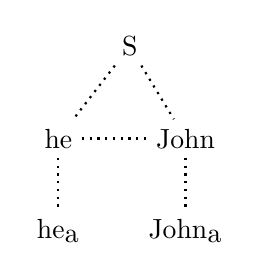
\begin{tikzpicture}[
    every node/.style={align=center},
    dotted line/.style={draw, dotted, thick},
    curved arrow/.style={draw, thick, -{Latex[bend]}},
    ]
\node (S) at (1.214084,0.000000) {S};
\node (he) at (0.307528,-1.171530) {he};
\node (John) at (1.922942,-1.171530) {John};
\draw[dotted line] (S) -- (he);
\draw[dotted line] (S) -- (John);
\draw[dotted line] (he) -- (John);
\node (heA) at (0.307528,-2.343060) {${\textrm{he}_{\textrm{a}}}$};
\node (JohnA) at (1.922942,-2.343060) {${\textrm{John}_{\textrm{a}}}$};
\draw[dotted line] (he) -- (heA);
\draw[dotted line] (John) -- (JohnA);
\end{tikzpicture}
}
\end{minipage}
\bigbreak

\clearpage

%%%%%%%%%%%%%%%%%%%%%%%%%%%%%%%%%%%%%%%%%%%%%%%%%%%%%%%%%%%%%%%%
%
%     (1.107) *He wasn't disturbed that Oscar was unpopular.
%
%%%%%%%%%%%%%%%%%%%%%%%%%%%%%%%%%%%%%%%%%%%%%%%%%%%%%%%%%%%%%%%%

\section*{(1.107) *He wasn't disturbed that Oscar was unpopular.}
\addcontentsline{toc}{section}{(1.107) *He wasn't disturbed that Oscar was unpopular.}

\bigbreak
\begin{enumerate*}
\item[(1.107)] *He wasn't disturbed that Oscar was unpopular.
\end{enumerate*}
\bigbreak

\bigbreak
\begin{minipage}{\textwidth}
\makebox[\textwidth][c]{
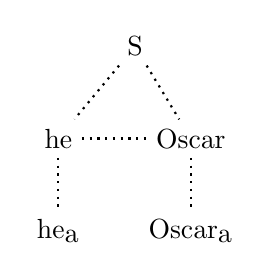
\begin{tikzpicture}[
    every node/.style={align=center},
    dotted line/.style={draw, dotted, thick},
    curved arrow/.style={draw, thick, -{Latex[bend]}},
    ]
\node (S) at (1.281446,0.000000) {S};
\node (he) at (0.307528,-1.171530) {he};
\node (Oscar) at (1.990305,-1.171530) {Oscar};
\draw[dotted line] (S) -- (he);
\draw[dotted line] (S) -- (Oscar);
\draw[dotted line] (he) -- (Oscar);
\node (heA) at (0.307528,-2.343060) {${\textrm{he}_{\textrm{a}}}$};
\node (OscarA) at (1.990305,-2.343060) {${\textrm{Oscar}_{\textrm{a}}}$};
\draw[dotted line] (he) -- (heA);
\draw[dotted line] (Oscar) -- (OscarA);
\end{tikzpicture}
}
\end{minipage}
\bigbreak

\clearpage

%%%%%%%%%%%%%%%%%%%%%%%%%%%%%%%%%%%%%%%%%%%%%%%%%%%%%%%%%%%%%%%%
%
%     (1.108) *It would get him into trouble for your brother to refuse to pay taxes.
%
%%%%%%%%%%%%%%%%%%%%%%%%%%%%%%%%%%%%%%%%%%%%%%%%%%%%%%%%%%%%%%%%

\section*{(1.108) *It would get him into trouble for your brother to refuse to pay taxes.}
\addcontentsline{toc}{section}{(1.108) *It would get him into trouble for your brother to refuse to pay taxes.}

\bigbreak
\begin{enumerate*}
\item[(1.108)] *It would get him into trouble for your brother to refuse to pay taxes.
\end{enumerate*}
\bigbreak

\bigbreak
\begin{minipage}{\textwidth}
\makebox[\textwidth][c]{
\begin{tikzpicture}[
    every node/.style={align=center},
    dotted line/.style={draw, dotted, thick},
    curved arrow/.style={draw, thick, -{Latex[bend]}},
    ]
\node (S) at (5.263035,0.000000) {S};
\node (him) at (0.424682,-1.171530) {him};
\node (trouble) at (2.331028,-1.171530) {trouble};
\node (your) at (4.291557,-1.171530) {your};
\node (brother) at (6.272100,-1.171530) {brother};
\node (PHI) at (8.220426,-1.171530) {$\phi$};
\node (taxes) at (9.997902,-1.171530) {taxes};
\draw[dotted line] (S) -- (him);
\draw[dotted line] (S) -- (taxes);
\draw[dotted line] (him) -- (trouble);
\draw[dotted line] (trouble) -- (your);
\draw[dotted line] (your) -- (brother);
\draw[dotted line] (brother) -- (PHI);
\draw[dotted line] (PHI) -- (taxes);
\node (himA) at (0.424682,-2.343060) {${\textrm{him}_{\textrm{a}}}$};
\node (troubleA) at (2.331028,-2.343060) {${\textrm{trouble}_{\textrm{a}}}$};
\node (yourA) at (4.291557,-2.343060) {${\textrm{your}_{\textrm{a}}}$};
\node (brotherA) at (6.272100,-2.343060) {${\textrm{brother}_{\textrm{a}}}$};
\node (PHIA) at (8.220426,-2.343060) {${\phi_{\textrm{a}}}$};
\node (taxesA) at (9.997902,-2.343060) {${\textrm{taxes}_{\textrm{a}}}$};
\draw[dotted line] (him) -- (himA);
\draw[dotted line] (trouble) -- (troubleA);
\draw[dotted line] (your) -- (yourA);
\draw[dotted line] (brother) -- (brotherA);
\draw[dotted line] (PHI) -- (PHIA);
\draw[dotted line] (taxes) -- (taxesA);
\node (himB) at (0.424682,-3.514590) {${\textrm{him}_{\textrm{b}}}$};
\node (troubleB) at (2.331028,-3.514590) {${\textrm{trouble}_{\textrm{b}}}$};
\node (brotherB) at (6.272100,-3.514590) {${\textrm{brother}_{\textrm{b}}}$};
\draw[dotted line] (himA) -- (himB);
\draw[dotted line] (troubleA) -- (troubleB);
\draw[dotted line] (brotherA) -- (brotherB);
\draw[curved arrow] (brotherB.north east) to [out=58.59,in=-88.02] (PHIA.south);
\draw[curved arrow] (troubleB.north east) to [out=28.62,in=-163.00] (PHIA.west);
\draw[curved arrow] (himB.east) to [out=22.26,in=133.82] (PHIA.north west);
\end{tikzpicture}
}
\end{minipage}
\bigbreak

\clearpage

%%%%%%%%%%%%%%%%%%%%%%%%%%%%%%%%%%%%%%%%%%%%%%%%%%%%%%%%%%%%%%%%
%
%     (1.109) *He was infuriated at Anna's complaining about Peter.
%
%%%%%%%%%%%%%%%%%%%%%%%%%%%%%%%%%%%%%%%%%%%%%%%%%%%%%%%%%%%%%%%%

\section*{(1.109) *He was infuriated at Anna's complaining about Peter.}
\addcontentsline{toc}{section}{(1.109) *He was infuriated at Anna's complaining about Peter.}

\bigbreak
\begin{enumerate*}
\item[(1.109)] *He was infuriated at Anna's complaining about Peter.
\end{enumerate*}
\bigbreak

\bigbreak
\begin{minipage}{\textwidth}
\makebox[\textwidth][c]{
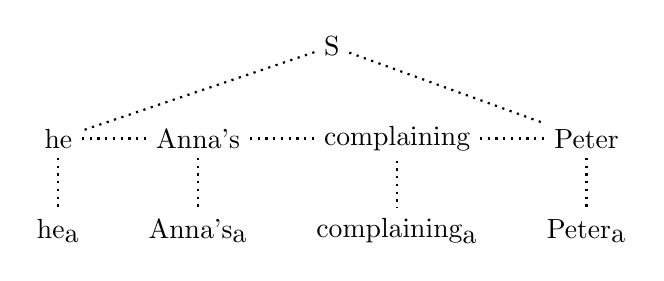
\begin{tikzpicture}[
    every node/.style={align=center},
    dotted line/.style={draw, dotted, thick},
    curved arrow/.style={draw, thick, -{Latex[bend]}},
    ]
\node (S) at (3.780395,0.000000) {S};
\node (he) at (0.307528,-1.171530) {he};
\node (Anna's) at (2.082564,-1.171530) {Anna's};
\node (complaining) at (4.609336,-1.171530) {complaining};
\node (Peter) at (7.016026,-1.171530) {Peter};
\draw[dotted line] (S) -- (he);
\draw[dotted line] (S) -- (Peter);
\draw[dotted line] (he) -- (Anna's);
\draw[dotted line] (Anna's) -- (complaining);
\draw[dotted line] (complaining) -- (Peter);
\node (heA) at (0.307528,-2.343060) {${\textrm{he}_{\textrm{a}}}$};
\node (Anna'sA) at (2.082564,-2.343060) {${\textrm{Anna's}_{\textrm{a}}}$};
\node (complainingA) at (4.609336,-2.343060) {${\textrm{complaining}_{\textrm{a}}}$};
\node (PeterA) at (7.016026,-2.343060) {${\textrm{Peter}_{\textrm{a}}}$};
\draw[dotted line] (he) -- (heA);
\draw[dotted line] (Anna's) -- (Anna'sA);
\draw[dotted line] (complaining) -- (complainingA);
\draw[dotted line] (Peter) -- (PeterA);
\end{tikzpicture}
}
\end{minipage}
\bigbreak

\clearpage

%%%%%%%%%%%%%%%%%%%%%%%%%%%%%%%%%%%%%%%%%%%%%%%%%%%%%%%%%%%%%%%%
%
%     (1.110) *He isn't bothered by the possibility that Fred will be unpopular.
%
%%%%%%%%%%%%%%%%%%%%%%%%%%%%%%%%%%%%%%%%%%%%%%%%%%%%%%%%%%%%%%%%

\section*{(1.110) *He isn't bothered by the possibility that Fred will be unpopular.}
\addcontentsline{toc}{section}{(1.110) *He isn't bothered by the possibility that Fred will be unpopular.}

\bigbreak
\begin{enumerate*}
\item[(1.110)] *He isn't bothered by the possibility that Fred will be unpopular.
\end{enumerate*}
\bigbreak

\bigbreak
\begin{minipage}{\textwidth}
\makebox[\textwidth][c]{
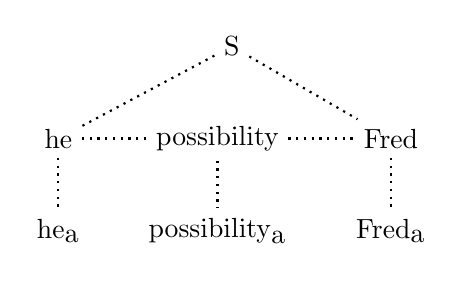
\begin{tikzpicture}[
    every node/.style={align=center},
    dotted line/.style={draw, dotted, thick},
    curved arrow/.style={draw, thick, -{Latex[bend]}},
    ]
\node (S) at (2.511151,0.000000) {S};
\node (he) at (0.307528,-1.171530) {he};
\node (possibility) at (2.327610,-1.171530) {possibility};
\node (Fred) at (4.531234,-1.171530) {Fred};
\draw[dotted line] (S) -- (he);
\draw[dotted line] (S) -- (Fred);
\draw[dotted line] (he) -- (possibility);
\draw[dotted line] (possibility) -- (Fred);
\node (heA) at (0.307528,-2.343060) {${\textrm{he}_{\textrm{a}}}$};
\node (possibilityA) at (2.327610,-2.343060) {${\textrm{possibility}_{\textrm{a}}}$};
\node (FredA) at (4.531234,-2.343060) {${\textrm{Fred}_{\textrm{a}}}$};
\draw[dotted line] (he) -- (heA);
\draw[dotted line] (possibility) -- (possibilityA);
\draw[dotted line] (Fred) -- (FredA);
\end{tikzpicture}
}
\end{minipage}
\bigbreak

\clearpage

%%%%%%%%%%%%%%%%%%%%%%%%%%%%%%%%%%%%%%%%%%%%%%%%%%%%%%%%%%%%%%%%
%
%     (1.111) Penelope cursed Peter and slandered him.
%
%%%%%%%%%%%%%%%%%%%%%%%%%%%%%%%%%%%%%%%%%%%%%%%%%%%%%%%%%%%%%%%%

\section*{(1.111) Penelope cursed Peter and slandered him.}
\addcontentsline{toc}{section}{(1.111) Penelope cursed Peter and slandered him.}

\bigbreak
\begin{enumerate*}
\item[(1.111)] Penelope cursed Peter and slandered him.
\end{enumerate*}
\bigbreak

\bigbreak
\begin{minipage}{\textwidth}
\makebox[\textwidth][c]{
\begin{tikzpicture}[
    every node/.style={align=center},
    dotted line/.style={draw, dotted, thick},
    curved arrow/.style={draw, thick, -{Latex[bend]}},
    ]
\node (S) at (3.437719,0.000000) {S};
\node (Penelope) at (0.817634,-1.171530) {Penelope};
\node (Peter) at (2.982693,-1.171530) {Peter};
\node (PHI) at (4.776766,-1.171530) {$\phi$};
\node (him) at (6.450757,-1.171530) {him};
\draw[dotted line] (S) -- (Penelope);
\draw[dotted line] (S) -- (him);
\draw[dotted line] (Penelope) -- (Peter);
\draw[dotted line] (Peter) -- (PHI);
\draw[dotted line] (PHI) -- (him);
\node (PenelopeA) at (0.817634,-2.343060) {${\textrm{Penelope}_{\textrm{a}}}$};
\node (PeterA) at (2.982693,-2.343060) {${\textrm{Peter}_{\textrm{a}}}$};
\node (PHIA) at (4.776766,-2.343060) {${\phi_{\textrm{a}}}$};
\node (himA) at (6.450757,-2.343060) {${\textrm{him}_{\textrm{a}}}$};
\draw[dotted line] (Penelope) -- (PenelopeA);
\draw[dotted line] (Peter) -- (PeterA);
\draw[dotted line] (PHI) -- (PHIA);
\draw[dotted line] (him) -- (himA);
\node (PenelopeB) at (0.817634,-3.514590) {${\textrm{Penelope}_{\textrm{b}}}$};
\node (PeterB) at (2.982693,-3.514590) {${\textrm{Peter}_{\textrm{b}}}$};
\draw[dotted line] (PenelopeA) -- (PenelopeB);
\draw[dotted line] (PeterA) -- (PeterB);
\node (PeterC) at (2.982693,-4.686120) {${\textrm{Peter}_{\textrm{c}}}$};
\draw[dotted line] (PeterB) -- (PeterC);
\draw[curved arrow] (PeterC.north) to [out=73.02,in=-70.41] (PHIA.south);
\draw[curved arrow] (PenelopeB.north east) to [out=39.31,in=-177.27] (PHIA.west);
\draw[curved arrow] (PeterB.north east) to [out=39.31,in=-140.69] (himA.south west);
\end{tikzpicture}
}
\end{minipage}
\bigbreak

\clearpage

%%%%%%%%%%%%%%%%%%%%%%%%%%%%%%%%%%%%%%%%%%%%%%%%%%%%%%%%%%%%%%%%
%
%     (1.112) *Penelope cursed him and slandered Peter.
%
%%%%%%%%%%%%%%%%%%%%%%%%%%%%%%%%%%%%%%%%%%%%%%%%%%%%%%%%%%%%%%%%

\section*{(1.112) *Penelope cursed him and slandered Peter.}
\addcontentsline{toc}{section}{(1.112) *Penelope cursed him and slandered Peter.}

\bigbreak
\begin{enumerate*}
\item[(1.112)] *Penelope cursed him and slandered Peter.
\end{enumerate*}
\bigbreak

\bigbreak
\begin{minipage}{\textwidth}
\makebox[\textwidth][c]{
\begin{tikzpicture}[
    every node/.style={align=center},
    dotted line/.style={draw, dotted, thick},
    curved arrow/.style={draw, thick, -{Latex[bend]}},
    ]
\node (S) at (3.437719,0.000000) {S};
\node (Penelope) at (0.817634,-1.171530) {Penelope};
\node (him) at (2.862611,-1.171530) {him};
\node (PHI) at (4.536602,-1.171530) {$\phi$};
\node (Peter) at (6.330675,-1.171530) {Peter};
\draw[dotted line] (S) -- (Penelope);
\draw[dotted line] (S) -- (Peter);
\draw[dotted line] (Penelope) -- (him);
\draw[dotted line] (him) -- (PHI);
\draw[dotted line] (PHI) -- (Peter);
\node (PenelopeA) at (0.817634,-2.343060) {${\textrm{Penelope}_{\textrm{a}}}$};
\node (himA) at (2.862611,-2.343060) {${\textrm{him}_{\textrm{a}}}$};
\node (PHIA) at (4.536602,-2.343060) {${\phi_{\textrm{a}}}$};
\node (PeterA) at (6.330675,-2.343060) {${\textrm{Peter}_{\textrm{a}}}$};
\draw[dotted line] (Penelope) -- (PenelopeA);
\draw[dotted line] (him) -- (himA);
\draw[dotted line] (PHI) -- (PHIA);
\draw[dotted line] (Peter) -- (PeterA);
\node (PenelopeB) at (0.817634,-3.514590) {${\textrm{Penelope}_{\textrm{b}}}$};
\node (himB) at (2.862611,-3.514590) {${\textrm{him}_{\textrm{b}}}$};
\draw[dotted line] (PenelopeA) -- (PenelopeB);
\draw[dotted line] (himA) -- (himB);
\draw[curved arrow] (himB.north east) to [out=58.59,in=-81.23] (PHIA.south);
\draw[curved arrow] (PenelopeB.north east) to [out=39.31,in=179.13] (PHIA.west);
\end{tikzpicture}
}
\end{minipage}
\bigbreak

\clearpage

%%%%%%%%%%%%%%%%%%%%%%%%%%%%%%%%%%%%%%%%%%%%%%%%%%%%%%%%%%%%%%%%
%
%     (1.113) The interest in visiting Las Vegas that Mary displayed is typical of gamblers.
%
%%%%%%%%%%%%%%%%%%%%%%%%%%%%%%%%%%%%%%%%%%%%%%%%%%%%%%%%%%%%%%%%

\section*{(1.113) The interest in visiting Las Vegas that Mary displayed is typical of gamblers.}
\addcontentsline{toc}{section}{(1.113) The interest in visiting Las Vegas that Mary displayed is typical of gamblers.}

\bigbreak
\begin{enumerate*}
\item[(1.113)] The interest in visiting Las Vegas that Mary displayed is typical of gamblers.
\end{enumerate*}
\bigbreak

\bigbreak
\begin{minipage}{\textwidth}
\makebox[\textwidth][c]{
\begin{tikzpicture}[
    every node/.style={align=center},
    dotted line/.style={draw, dotted, thick},
    curved arrow/.style={draw, thick, -{Latex[bend]}},
    ]
\node (S) at (6.090432,0.000000) {S};
\node (interest) at (0.709267,-1.171530) {interest};
\node (PHI1) at (2.755708,-1.171530) {${\phi_{\textrm{1}}}$};
\node (Las Vegas) at (5.039386,-1.171530) {Las Vegas};
\node (Mary) at (7.330874,-1.171530) {Mary};
\node (PHI2) at (9.210373,-1.171530) {${\phi_{\textrm{2}}}$};
\node (gamblers) at (11.364205,-1.171530) {gamblers};
\draw[dotted line] (S) -- (interest);
\draw[dotted line] (S) -- (gamblers);
\draw[dotted line] (interest) -- (PHI1);
\draw[dotted line] (PHI1) -- (Las Vegas);
\draw[dotted line] (Las Vegas) -- (Mary);
\draw[dotted line] (Mary) -- (PHI2);
\draw[dotted line] (PHI2) -- (gamblers);
\node (interestA) at (0.709267,-2.343060) {${\textrm{interest}_{\textrm{a}}}$};
\node (PHI1A) at (2.755708,-2.343060) {${\phi_{\textrm{1a}}}$};
\node (Las VegasA) at (5.039386,-2.343060) {${\textrm{Las Vegas}_{\textrm{a}}}$};
\node (MaryA) at (7.330874,-2.343060) {${\textrm{Mary}_{\textrm{a}}}$};
\node (PHI2A) at (9.210373,-2.343060) {${\phi_{\textrm{2a}}}$};
\node (gamblersA) at (11.364205,-2.343060) {${\textrm{gamblers}_{\textrm{a}}}$};
\draw[dotted line] (interest) -- (interestA);
\draw[dotted line] (PHI1) -- (PHI1A);
\draw[dotted line] (Las Vegas) -- (Las VegasA);
\draw[dotted line] (Mary) -- (MaryA);
\draw[dotted line] (PHI2) -- (PHI2A);
\draw[dotted line] (gamblers) -- (gamblersA);
\node (interestB) at (0.709267,-3.514590) {${\textrm{interest}_{\textrm{b}}}$};
\node (PHI1B) at (2.755708,-3.514590) {${\phi_{\textrm{1b}}}$};
\node (Las VegasB) at (5.039386,-3.514590) {${\textrm{Las Vegas}_{\textrm{b}}}$};
\node (MaryB) at (7.330874,-3.514590) {${\textrm{Mary}_{\textrm{b}}}$};
\node (PHI2B) at (9.210373,-3.514590) {${\phi_{\textrm{2b}}}$};
\node (gamblersB) at (11.364205,-3.514590) {${\textrm{gamblers}_{\textrm{b}}}$};
\draw[dotted line] (interestA) -- (interestB);
\draw[dotted line] (PHI1A) -- (PHI1B);
\draw[dotted line] (Las VegasA) -- (Las VegasB);
\draw[dotted line] (MaryA) -- (MaryB);
\draw[dotted line] (PHI2A) -- (PHI2B);
\draw[dotted line] (gamblersA) -- (gamblersB);
\node (interestC) at (0.709267,-4.686120) {${\textrm{interest}_{\textrm{c}}}$};
\node (MaryC) at (7.330874,-4.686120) {${\textrm{Mary}_{\textrm{c}}}$};
\node (PHI2C) at (9.210373,-4.686120) {${\phi_{\textrm{2c}}}$};
\node (gamblersC) at (11.364205,-4.686120) {${\textrm{gamblers}_{\textrm{c}}}$};
\draw[dotted line] (interestB) -- (interestC);
\draw[dotted line] (MaryB) -- (MaryC);
\draw[dotted line] (PHI2B) -- (PHI2C);
\draw[dotted line] (gamblersB) -- (gamblersC);
\node (interestD) at (0.709267,-5.857650) {${\textrm{interest}_{\textrm{d}}}$};
\node (gamblersD) at (11.364205,-5.857650) {${\textrm{gamblers}_{\textrm{d}}}$};
\draw[dotted line] (interestC) -- (interestD);
\draw[dotted line] (gamblersC) -- (gamblersD);
\draw[curved arrow] (gamblersB.north west) to [out=121.41,in=-55.09] (PHI2A.south east);
\draw[curved arrow] (Las VegasB.north east) to [out=39.31,in=-141.15] (PHI2A.south west);
\draw[curved arrow] (PHI1B.north east) to [out=28.62,in=168.51] (PHI2A.west);
\draw[curved arrow] (interestB.east) to [out=22.26,in=120.33] (PHI2A.north west);
\draw[curved arrow] (PHI2B.north west) to [out=151.38,in=58.08] (PHI1A.north east);
\draw[curved arrow] (gamblersC.north west) to [out=140.69,in=-37.26] (PHI1A.south east);
\draw[curved arrow] (MaryB.north west) to [out=140.69,in=7.74] (PHI1A.east);
\draw[curved arrow] (interestC.north) to [out=73.02,in=-116.10] (PHI1A.south west);
\draw[curved arrow] (PHI2C.north west) to [out=151.38,in=58.08] (PHI1B.north east);
\draw[curved arrow] (gamblersD.north west) to [out=140.69,in=-37.26] (PHI1B.south east);
\draw[curved arrow] (MaryC.north west) to [out=140.69,in=7.74] (PHI1B.east);
\draw[curved arrow] (interestD.north) to [out=73.02,in=-116.10] (PHI1B.south west);
\end{tikzpicture}
}
\end{minipage}
\bigbreak

\clearpage

%%%%%%%%%%%%%%%%%%%%%%%%%%%%%%%%%%%%%%%%%%%%%%%%%%%%%%%%%%%%%%%%
%
%     (5.2) June hates flowers, but she waters them anyway.
%
%%%%%%%%%%%%%%%%%%%%%%%%%%%%%%%%%%%%%%%%%%%%%%%%%%%%%%%%%%%%%%%%

\section*{(5.2) June hates flowers, but she waters them anyway.}
\addcontentsline{toc}{section}{(5.2) June hates flowers, but she waters them anyway.}

\bigbreak
\begin{enumerate*}
\item[(5.2)] June hates flowers, but she waters them anyway.
\end{enumerate*}
\bigbreak

\bigbreak
\begin{minipage}{\textwidth}
\makebox[\textwidth][c]{
\begin{tikzpicture}[
    every node/.style={align=center},
    dotted line/.style={draw, dotted, thick},
    curved arrow/.style={draw, thick, -{Latex[bend]}},
    ]
\node (S) at (3.263941,0.000000) {S};
\node (June) at (0.495462,-1.171530) {June};
\node (flowers) at (2.458919,-1.171530) {flowers};
\node (she) at (4.303759,-1.171530) {she};
\node (them) at (6.005573,-1.171530) {them};
\draw[dotted line] (S) -- (June);
\draw[dotted line] (S) -- (them);
\draw[dotted line] (June) -- (flowers);
\draw[dotted line] (flowers) -- (she);
\draw[dotted line] (she) -- (them);
\node (JuneA) at (0.495462,-2.343060) {${\textrm{June}_{\textrm{a}}}$};
\node (flowersA) at (2.458919,-2.343060) {${\textrm{flowers}_{\textrm{a}}}$};
\node (sheA) at (4.303759,-2.343060) {${\textrm{she}_{\textrm{a}}}$};
\node (themA) at (6.005573,-2.343060) {${\textrm{them}_{\textrm{a}}}$};
\draw[dotted line] (June) -- (JuneA);
\draw[dotted line] (flowers) -- (flowersA);
\draw[dotted line] (she) -- (sheA);
\draw[dotted line] (them) -- (themA);
\node (JuneB) at (0.495462,-3.514590) {${\textrm{June}_{\textrm{b}}}$};
\node (flowersB) at (2.458919,-3.514590) {${\textrm{flowers}_{\textrm{b}}}$};
\draw[dotted line] (JuneA) -- (JuneB);
\draw[dotted line] (flowersA) -- (flowersB);
\draw[curved arrow] (JuneB.north east) to [out=39.31,in=-140.69] (sheA.south west);
\draw[curved arrow] (flowersB.north east) to [out=39.31,in=-140.69] (themA.south west);
\end{tikzpicture}
}
\end{minipage}
\bigbreak

\clearpage

%%%%%%%%%%%%%%%%%%%%%%%%%%%%%%%%%%%%%%%%%%%%%%%%%%%%%%%%%%%%%%%%
%
%     (8.1) John wants to give June a present, but he isn't sure she’ll like it.
%
%%%%%%%%%%%%%%%%%%%%%%%%%%%%%%%%%%%%%%%%%%%%%%%%%%%%%%%%%%%%%%%%

\section*{(8.1) John wants to give June a present, but he isn't sure she’ll like it.}
\addcontentsline{toc}{section}{(8.1) John wants to give June a present, but he isn't sure she’ll like it.}

\bigbreak
\begin{enumerate*}
\item[(8.1)] John wants to give June a present, but he isn't sure she’ll like it.
\end{enumerate*}
\bigbreak

\bigbreak
\begin{minipage}{\textwidth}
\makebox[\textwidth][c]{
\begin{tikzpicture}[
    every node/.style={align=center},
    dotted line/.style={draw, dotted, thick},
    curved arrow/.style={draw, thick, -{Latex[bend]}},
    ]
\node (S) at (5.478383,0.000000) {S};
\node (John) at (0.505225,-1.171530) {John};
\node (PHI) at (2.259759,-1.171530) {$\phi$};
\node (June) at (4.004530,-1.171530) {June};
\node (present) at (5.992394,-1.171530) {present};
\node (he) at (7.792325,-1.171530) {he};
\node (she) at (9.279357,-1.171530) {she};
\node (it) at (10.707813,-1.171530) {it};
\draw[dotted line] (S) -- (John);
\draw[dotted line] (S) -- (it);
\draw[dotted line] (John) -- (PHI);
\draw[dotted line] (PHI) -- (June);
\draw[dotted line] (June) -- (present);
\draw[dotted line] (present) -- (he);
\draw[dotted line] (he) -- (she);
\draw[dotted line] (she) -- (it);
\node (JohnA) at (0.505225,-2.343060) {${\textrm{John}_{\textrm{a}}}$};
\node (PHIA) at (2.259759,-2.343060) {${\phi_{\textrm{a}}}$};
\node (JuneA) at (4.004530,-2.343060) {${\textrm{June}_{\textrm{a}}}$};
\node (presentA) at (5.992394,-2.343060) {${\textrm{present}_{\textrm{a}}}$};
\node (heA) at (7.792325,-2.343060) {${\textrm{he}_{\textrm{a}}}$};
\node (sheA) at (9.279357,-2.343060) {${\textrm{she}_{\textrm{a}}}$};
\node (itA) at (10.707813,-2.343060) {${\textrm{it}_{\textrm{a}}}$};
\draw[dotted line] (John) -- (JohnA);
\draw[dotted line] (PHI) -- (PHIA);
\draw[dotted line] (June) -- (JuneA);
\draw[dotted line] (present) -- (presentA);
\draw[dotted line] (he) -- (heA);
\draw[dotted line] (she) -- (sheA);
\draw[dotted line] (it) -- (itA);
\node (JohnB) at (0.505225,-3.514590) {${\textrm{John}_{\textrm{b}}}$};
\node (PHIB) at (2.259759,-3.514590) {${\phi_{\textrm{b}}}$};
\node (JuneB) at (4.004530,-3.514590) {${\textrm{June}_{\textrm{b}}}$};
\node (presentB) at (5.992394,-3.514590) {${\textrm{present}_{\textrm{b}}}$};
\draw[dotted line] (JohnA) -- (JohnB);
\draw[dotted line] (PHIA) -- (PHIB);
\draw[dotted line] (JuneA) -- (JuneB);
\draw[dotted line] (presentA) -- (presentB);
\node (JohnC) at (0.505225,-4.686120) {${\textrm{John}_{\textrm{c}}}$};
\node (PHIC) at (2.259759,-4.686120) {${\phi_{\textrm{c}}}$};
\draw[dotted line] (JohnB) -- (JohnC);
\draw[dotted line] (PHIB) -- (PHIC);
\node (JohnD) at (0.505225,-5.857650) {${\textrm{John}_{\textrm{d}}}$};
\node (PHID) at (2.259759,-5.857650) {${\phi_{\textrm{d}}}$};
\draw[dotted line] (JohnC) -- (JohnD);
\draw[dotted line] (PHIC) -- (PHID);
\draw[curved arrow] (PHID.north east) to [out=58.59,in=-85.50] (heA.south);
\draw[curved arrow] (JohnB.east) to [out=22.26,in=166.34] (heA.west);
\draw[curved arrow] (presentB.north east) to [out=28.62,in=-109.00] (itA.south);
\draw[curved arrow] (PHIB.east) to [out=18.13,in=155.75] (itA.north west);
\draw[curved arrow] (PHIC.north east) to [out=39.31,in=-98.36] (sheA.south);
\draw[curved arrow] (JuneB.north east) to [out=28.62,in=166.29] (sheA.west);
\draw[curved arrow] (JohnC.north) to [out=73.02,in=-106.98] (PHIA.south);
\draw[curved arrow] (JohnD.east) to [out=0.00,in=-180.00] (PHID.west);
\end{tikzpicture}
}
\end{minipage}
\bigbreak

\clearpage

%%%%%%%%%%%%%%%%%%%%%%%%%%%%%%%%%%%%%%%%%%%%%%%%%%%%%%%%%%%%%%%%
%
%     (10.1) John wants to give June a present, but he isn't sure she’ll like it.
%
%%%%%%%%%%%%%%%%%%%%%%%%%%%%%%%%%%%%%%%%%%%%%%%%%%%%%%%%%%%%%%%%

\section*{(10.1) John wants to give June a present, but he isn't sure she’ll like it.}
\addcontentsline{toc}{section}{(10.1) John wants to give June a present, but he isn't sure she’ll like it.}

\bigbreak
\begin{enumerate*}
\item[(10.1)] John wants to give June a present, but he isn't sure she’ll like it.
\end{enumerate*}
\bigbreak

\bigbreak
\begin{minipage}{\textwidth}
\makebox[\textwidth][c]{
\begin{tikzpicture}[
    every node/.style={align=center},
    dotted line/.style={draw, dotted, thick},
    curved arrow/.style={draw, thick, -{Latex[bend]}},
    ]
\node (S) at (5.478383,0.000000) {S};
\node (John) at (0.505225,-1.171530) {John};
\node (PHI) at (2.259759,-1.171530) {$\phi$};
\node (June) at (4.004530,-1.171530) {June};
\node (present) at (5.992394,-1.171530) {present};
\node (he) at (7.792325,-1.171530) {he};
\node (she) at (9.279357,-1.171530) {she};
\node (it) at (10.707813,-1.171530) {it};
\draw[dotted line] (S) -- (John);
\draw[dotted line] (S) -- (it);
\draw[dotted line] (John) -- (PHI);
\draw[dotted line] (PHI) -- (June);
\draw[dotted line] (June) -- (present);
\draw[dotted line] (present) -- (he);
\draw[dotted line] (he) -- (she);
\draw[dotted line] (she) -- (it);
\node (JohnA) at (0.505225,-2.343060) {${\textrm{John}_{\textrm{a}}}$};
\node (PHIA) at (2.259759,-2.343060) {${\phi_{\textrm{a}}}$};
\node (JuneA) at (4.004530,-2.343060) {${\textrm{June}_{\textrm{a}}}$};
\node (presentA) at (5.992394,-2.343060) {${\textrm{present}_{\textrm{a}}}$};
\node (heA) at (7.792325,-2.343060) {${\textrm{he}_{\textrm{a}}}$};
\node (sheA) at (9.279357,-2.343060) {${\textrm{she}_{\textrm{a}}}$};
\node (itA) at (10.707813,-2.343060) {${\textrm{it}_{\textrm{a}}}$};
\draw[dotted line] (John) -- (JohnA);
\draw[dotted line] (PHI) -- (PHIA);
\draw[dotted line] (June) -- (JuneA);
\draw[dotted line] (present) -- (presentA);
\draw[dotted line] (he) -- (heA);
\draw[dotted line] (she) -- (sheA);
\draw[dotted line] (it) -- (itA);
\node (JohnB) at (0.505225,-3.514590) {${\textrm{John}_{\textrm{b}}}$};
\node (PHIB) at (2.259759,-3.514590) {${\phi_{\textrm{b}}}$};
\node (JuneB) at (4.004530,-3.514590) {${\textrm{June}_{\textrm{b}}}$};
\node (presentB) at (5.992394,-3.514590) {${\textrm{present}_{\textrm{b}}}$};
\draw[dotted line] (JohnA) -- (JohnB);
\draw[dotted line] (PHIA) -- (PHIB);
\draw[dotted line] (JuneA) -- (JuneB);
\draw[dotted line] (presentA) -- (presentB);
\node (JohnC) at (0.505225,-4.686120) {${\textrm{John}_{\textrm{c}}}$};
\node (PHIC) at (2.259759,-4.686120) {${\phi_{\textrm{c}}}$};
\draw[dotted line] (JohnB) -- (JohnC);
\draw[dotted line] (PHIB) -- (PHIC);
\node (JohnD) at (0.505225,-5.857650) {${\textrm{John}_{\textrm{d}}}$};
\node (PHID) at (2.259759,-5.857650) {${\phi_{\textrm{d}}}$};
\draw[dotted line] (JohnC) -- (JohnD);
\draw[dotted line] (PHIC) -- (PHID);
\draw[curved arrow] (PHID.north east) to [out=58.59,in=-85.50] (heA.south);
\draw[curved arrow] (JohnB.east) to [out=22.26,in=166.34] (heA.west);
\draw[curved arrow] (presentB.north east) to [out=28.62,in=-109.00] (itA.south);
\draw[curved arrow] (PHIB.east) to [out=18.13,in=155.75] (itA.north west);
\draw[curved arrow] (PHIC.north east) to [out=39.31,in=-98.36] (sheA.south);
\draw[curved arrow] (JuneB.north east) to [out=28.62,in=166.29] (sheA.west);
\draw[curved arrow] (JohnC.north) to [out=73.02,in=-106.98] (PHIA.south);
\draw[curved arrow] (JohnD.east) to [out=0.00,in=-180.00] (PHID.west);
\end{tikzpicture}
}
\end{minipage}
\bigbreak

\clearpage

%%%%%%%%%%%%%%%%%%%%%%%%%%%%%%%%%%%%%%%%%%%%%%%%%%%%%%%%%%%%%%%%
%
%     (10.2) Janet saw herself.
%
%%%%%%%%%%%%%%%%%%%%%%%%%%%%%%%%%%%%%%%%%%%%%%%%%%%%%%%%%%%%%%%%

\section*{(10.2) Janet saw herself.}
\addcontentsline{toc}{section}{(10.2) Janet saw herself.}

\bigbreak
\begin{enumerate*}
\item[(10.2)] Janet saw herself.
\end{enumerate*}
\bigbreak

\bigbreak
\begin{minipage}{\textwidth}
\makebox[\textwidth][c]{
\begin{tikzpicture}[
    every node/.style={align=center},
    dotted line/.style={draw, dotted, thick},
    curved arrow/.style={draw, thick, -{Latex[bend]}},
    ]
\node (S) at (1.581653,0.000000) {S};
\node (Janet) at (0.554039,-1.171530) {Janet};
\node (herself) at (2.537022,-1.171530) {herself};
\draw[dotted line] (S) -- (Janet);
\draw[dotted line] (S) -- (herself);
\draw[dotted line] (Janet) -- (herself);
\node (JanetA) at (0.554039,-2.343060) {${\textrm{Janet}_{\textrm{a}}}$};
\node (herselfA) at (2.537022,-2.343060) {${\textrm{herself}_{\textrm{a}}}$};
\draw[dotted line] (Janet) -- (JanetA);
\draw[dotted line] (herself) -- (herselfA);
\node (JanetB) at (0.554039,-3.514590) {${\textrm{Janet}_{\textrm{b}}}$};
\draw[dotted line] (JanetA) -- (JanetB);
\draw[curved arrow] (JanetB.north east) to [out=58.59,in=-121.41] (herselfA.south west);
\end{tikzpicture}
}
\end{minipage}
\bigbreak

\clearpage

%%%%%%%%%%%%%%%%%%%%%%%%%%%%%%%%%%%%%%%%%%%%%%%%%%%%%%%%%%%%%%%%
%
%     (10.3) Janet saw her.
%
%%%%%%%%%%%%%%%%%%%%%%%%%%%%%%%%%%%%%%%%%%%%%%%%%%%%%%%%%%%%%%%%

\section*{(10.3) Janet saw her.}
\addcontentsline{toc}{section}{(10.3) Janet saw her.}

\bigbreak
\begin{enumerate*}
\item[(10.3)] Janet saw her.
\end{enumerate*}
\bigbreak

\bigbreak
\begin{minipage}{\textwidth}
\makebox[\textwidth][c]{
\begin{tikzpicture}[
    every node/.style={align=center},
    dotted line/.style={draw, dotted, thick},
    curved arrow/.style={draw, thick, -{Latex[bend]}},
    ]
\node (S) at (1.331725,0.000000) {S};
\node (Janet) at (0.554039,-1.171530) {Janet};
\node (her) at (2.287094,-1.171530) {her};
\draw[dotted line] (S) -- (Janet);
\draw[dotted line] (S) -- (her);
\draw[dotted line] (Janet) -- (her);
\node (JanetA) at (0.554039,-2.343060) {${\textrm{Janet}_{\textrm{a}}}$};
\node (herA) at (2.287094,-2.343060) {${\textrm{her}_{\textrm{a}}}$};
\draw[dotted line] (Janet) -- (JanetA);
\draw[dotted line] (her) -- (herA);
\node (JanetB) at (0.554039,-3.514590) {${\textrm{Janet}_{\textrm{b}}}$};
\draw[dotted line] (JanetA) -- (JanetB);
\draw[curved arrow] (JanetB.north east) to [out=58.59,in=-121.41] (herA.south west);
\end{tikzpicture}
}
\end{minipage}
\bigbreak

\clearpage

%%%%%%%%%%%%%%%%%%%%%%%%%%%%%%%%%%%%%%%%%%%%%%%%%%%%%%%%%%%%%%%%
%
%     (10.4) *Janet saw himself.
%
%%%%%%%%%%%%%%%%%%%%%%%%%%%%%%%%%%%%%%%%%%%%%%%%%%%%%%%%%%%%%%%%

\section*{(10.4) *Janet saw himself.}
\addcontentsline{toc}{section}{(10.4) *Janet saw himself.}

\bigbreak
\begin{enumerate*}
\item[(10.4)] *Janet saw himself.
\end{enumerate*}
\bigbreak

\bigbreak
\begin{minipage}{\textwidth}
\makebox[\textwidth][c]{
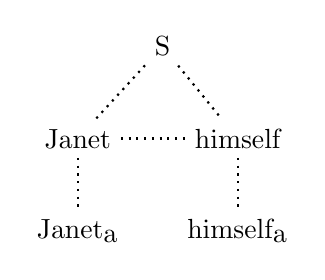
\begin{tikzpicture}[
    every node/.style={align=center},
    dotted line/.style={draw, dotted, thick},
    curved arrow/.style={draw, thick, -{Latex[bend]}},
    ]
\node (S) at (1.629979,0.000000) {S};
\node (Janet) at (0.554039,-1.171530) {Janet};
\node (himself) at (2.585348,-1.171530) {himself};
\draw[dotted line] (S) -- (Janet);
\draw[dotted line] (S) -- (himself);
\draw[dotted line] (Janet) -- (himself);
\node (JanetA) at (0.554039,-2.343060) {${\textrm{Janet}_{\textrm{a}}}$};
\node (himselfA) at (2.585348,-2.343060) {${\textrm{himself}_{\textrm{a}}}$};
\draw[dotted line] (Janet) -- (JanetA);
\draw[dotted line] (himself) -- (himselfA);
\end{tikzpicture}
}
\end{minipage}
\bigbreak

\clearpage

%%%%%%%%%%%%%%%%%%%%%%%%%%%%%%%%%%%%%%%%%%%%%%%%%%%%%%%%%%%%%%%%
%
%     (10.5) The men threw a smokescreen around themselves.
%
%%%%%%%%%%%%%%%%%%%%%%%%%%%%%%%%%%%%%%%%%%%%%%%%%%%%%%%%%%%%%%%%

\section*{(10.5) The men threw a smokescreen around themselves.}
\addcontentsline{toc}{section}{(10.5) The men threw a smokescreen around themselves.}

\bigbreak
\begin{enumerate*}
\item[(10.5)] The men threw a smokescreen around themselves.
\end{enumerate*}
\bigbreak

\bigbreak
\begin{minipage}{\textwidth}
\makebox[\textwidth][c]{
\begin{tikzpicture}[
    every node/.style={align=center},
    dotted line/.style={draw, dotted, thick},
    curved arrow/.style={draw, thick, -{Latex[bend]}},
    ]
\node (S) at (3.291685,0.000000) {S};
\node (men) at (0.453970,-1.171530) {men};
\node (smokescreen) at (2.786949,-1.171530) {smokescreen};
\node (themselves) at (5.624664,-1.171530) {themselves};
\draw[dotted line] (S) -- (men);
\draw[dotted line] (S) -- (themselves);
\draw[dotted line] (men) -- (smokescreen);
\draw[dotted line] (smokescreen) -- (themselves);
\node (menA) at (0.453970,-2.343060) {${\textrm{men}_{\textrm{a}}}$};
\node (smokescreenA) at (2.786949,-2.343060) {${\textrm{smokescreen}_{\textrm{a}}}$};
\node (themselvesA) at (5.624664,-2.343060) {${\textrm{themselves}_{\textrm{a}}}$};
\draw[dotted line] (men) -- (menA);
\draw[dotted line] (smokescreen) -- (smokescreenA);
\draw[dotted line] (themselves) -- (themselvesA);
\node (menB) at (0.453970,-3.514590) {${\textrm{men}_{\textrm{b}}}$};
\draw[dotted line] (menA) -- (menB);
\draw[curved arrow] (menB.north east) to [out=39.31,in=-140.69] (themselvesA.south west);
\end{tikzpicture}
}
\end{minipage}
\bigbreak

\clearpage

%%%%%%%%%%%%%%%%%%%%%%%%%%%%%%%%%%%%%%%%%%%%%%%%%%%%%%%%%%%%%%%%
%
%     (10.6) The men found a smokescreen around them.
%
%%%%%%%%%%%%%%%%%%%%%%%%%%%%%%%%%%%%%%%%%%%%%%%%%%%%%%%%%%%%%%%%

\section*{(10.6) The men found a smokescreen around them.}
\addcontentsline{toc}{section}{(10.6) The men found a smokescreen around them.}

\bigbreak
\begin{enumerate*}
\item[(10.6)] The men found a smokescreen around them.
\end{enumerate*}
\bigbreak

\bigbreak
\begin{minipage}{\textwidth}
\makebox[\textwidth][c]{
\begin{tikzpicture}[
    every node/.style={align=center},
    dotted line/.style={draw, dotted, thick},
    curved arrow/.style={draw, thick, -{Latex[bend]}},
    ]
\node (S) at (2.855289,0.000000) {S};
\node (men) at (0.453970,-1.171530) {men};
\node (smokescreen) at (2.786949,-1.171530) {smokescreen};
\node (them) at (5.188267,-1.171530) {them};
\draw[dotted line] (S) -- (men);
\draw[dotted line] (S) -- (them);
\draw[dotted line] (men) -- (smokescreen);
\draw[dotted line] (smokescreen) -- (them);
\node (menA) at (0.453970,-2.343060) {${\textrm{men}_{\textrm{a}}}$};
\node (smokescreenA) at (2.786949,-2.343060) {${\textrm{smokescreen}_{\textrm{a}}}$};
\node (themA) at (5.188267,-2.343060) {${\textrm{them}_{\textrm{a}}}$};
\draw[dotted line] (men) -- (menA);
\draw[dotted line] (smokescreen) -- (smokescreenA);
\draw[dotted line] (them) -- (themA);
\end{tikzpicture}
}
\end{minipage}
\bigbreak

\clearpage

%%%%%%%%%%%%%%%%%%%%%%%%%%%%%%%%%%%%%%%%%%%%%%%%%%%%%%%%%%%%%%%%
%
%     (10.7) The men found a smokescreen to be around them.
%
%%%%%%%%%%%%%%%%%%%%%%%%%%%%%%%%%%%%%%%%%%%%%%%%%%%%%%%%%%%%%%%%

\section*{(10.7) The men found a smokescreen to be around them.}
\addcontentsline{toc}{section}{(10.7) The men found a smokescreen to be around them.}

\bigbreak
\begin{enumerate*}
\item[(10.7)] The men found a smokescreen to be around them.
\end{enumerate*}
\bigbreak

\bigbreak
\begin{minipage}{\textwidth}
\makebox[\textwidth][c]{
\begin{tikzpicture}[
    every node/.style={align=center},
    dotted line/.style={draw, dotted, thick},
    curved arrow/.style={draw, thick, -{Latex[bend]}},
    ]
\node (S) at (2.855289,0.000000) {S};
\node (men) at (0.453970,-1.171530) {men};
\node (smokescreen) at (2.786949,-1.171530) {smokescreen};
\node (them) at (5.188267,-1.171530) {them};
\draw[dotted line] (S) -- (men);
\draw[dotted line] (S) -- (them);
\draw[dotted line] (men) -- (smokescreen);
\draw[dotted line] (smokescreen) -- (them);
\node (menA) at (0.453970,-2.343060) {${\textrm{men}_{\textrm{a}}}$};
\node (smokescreenA) at (2.786949,-2.343060) {${\textrm{smokescreen}_{\textrm{a}}}$};
\node (themA) at (5.188267,-2.343060) {${\textrm{them}_{\textrm{a}}}$};
\draw[dotted line] (men) -- (menA);
\draw[dotted line] (smokescreen) -- (smokescreenA);
\draw[dotted line] (them) -- (themA);
\node (menB) at (0.453970,-3.514590) {${\textrm{men}_{\textrm{b}}}$};
\draw[dotted line] (menA) -- (menB);
\draw[curved arrow] (menB.north east) to [out=39.31,in=-140.69] (themA.south west);
\end{tikzpicture}
}
\end{minipage}
\bigbreak

\clearpage

%%%%%%%%%%%%%%%%%%%%%%%%%%%%%%%%%%%%%%%%%%%%%%%%%%%%%%%%%%%%%%%%
%
%     (10.8) The men found a smokescreen and it was around them.
%
%%%%%%%%%%%%%%%%%%%%%%%%%%%%%%%%%%%%%%%%%%%%%%%%%%%%%%%%%%%%%%%%

\section*{(10.8) The men found a smokescreen and it was around them.}
\addcontentsline{toc}{section}{(10.8) The men found a smokescreen and it was around them.}

\bigbreak
\begin{enumerate*}
\item[(10.8)] The men found a smokescreen and it was around them.
\end{enumerate*}
\bigbreak

\bigbreak
\begin{minipage}{\textwidth}
\makebox[\textwidth][c]{
\begin{tikzpicture}[
    every node/.style={align=center},
    dotted line/.style={draw, dotted, thick},
    curved arrow/.style={draw, thick, -{Latex[bend]}},
    ]
\node (S) at (3.505571,0.000000) {S};
\node (men) at (0.453970,-1.171530) {men};
\node (smokescreen) at (2.786949,-1.171530) {smokescreen};
\node (it) at (4.914909,-1.171530) {it};
\node (them) at (6.488832,-1.171530) {them};
\draw[dotted line] (S) -- (men);
\draw[dotted line] (S) -- (them);
\draw[dotted line] (men) -- (smokescreen);
\draw[dotted line] (smokescreen) -- (it);
\draw[dotted line] (it) -- (them);
\node (menA) at (0.453970,-2.343060) {${\textrm{men}_{\textrm{a}}}$};
\node (smokescreenA) at (2.786949,-2.343060) {${\textrm{smokescreen}_{\textrm{a}}}$};
\node (itA) at (4.914909,-2.343060) {${\textrm{it}_{\textrm{a}}}$};
\node (themA) at (6.488832,-2.343060) {${\textrm{them}_{\textrm{a}}}$};
\draw[dotted line] (men) -- (menA);
\draw[dotted line] (smokescreen) -- (smokescreenA);
\draw[dotted line] (it) -- (itA);
\draw[dotted line] (them) -- (themA);
\node (menB) at (0.453970,-3.514590) {${\textrm{men}_{\textrm{b}}}$};
\node (smokescreenB) at (2.786949,-3.514590) {${\textrm{smokescreen}_{\textrm{b}}}$};
\draw[dotted line] (menA) -- (menB);
\draw[dotted line] (smokescreenA) -- (smokescreenB);
\draw[curved arrow] (menB.north east) to [out=28.62,in=-151.38] (themA.south west);
\draw[curved arrow] (smokescreenB.north east) to [out=58.59,in=-121.41] (itA.south west);
\end{tikzpicture}
}
\end{minipage}
\bigbreak

\clearpage

%%%%%%%%%%%%%%%%%%%%%%%%%%%%%%%%%%%%%%%%%%%%%%%%%%%%%%%%%%%%%%%%
%
%     (10.9) I told John to protect himself.
%
%%%%%%%%%%%%%%%%%%%%%%%%%%%%%%%%%%%%%%%%%%%%%%%%%%%%%%%%%%%%%%%%

\section*{(10.9) I told John to protect himself.}
\addcontentsline{toc}{section}{(10.9) I told John to protect himself.}

\bigbreak
\begin{enumerate*}
\item[(10.9)] I told John to protect himself.
\end{enumerate*}
\bigbreak

\bigbreak
\begin{minipage}{\textwidth}
\makebox[\textwidth][c]{
\begin{tikzpicture}[
    every node/.style={align=center},
    dotted line/.style={draw, dotted, thick},
    curved arrow/.style={draw, thick, -{Latex[bend]}},
    ]
\node (S) at (3.025730,0.000000) {S};
\node (I) at (0.195256,-1.171530) {I};
\node (John) at (1.698398,-1.171530) {John};
\node (PHI) at (3.452932,-1.171530) {$\phi$};
\node (himself) at (5.376851,-1.171530) {himself};
\draw[dotted line] (S) -- (I);
\draw[dotted line] (S) -- (himself);
\draw[dotted line] (I) -- (John);
\draw[dotted line] (John) -- (PHI);
\draw[dotted line] (PHI) -- (himself);
\node (IA) at (0.195256,-2.343060) {${\textrm{I}_{\textrm{a}}}$};
\node (JohnA) at (1.698398,-2.343060) {${\textrm{John}_{\textrm{a}}}$};
\node (PHIA) at (3.452932,-2.343060) {${\phi_{\textrm{a}}}$};
\node (himselfA) at (5.376851,-2.343060) {${\textrm{himself}_{\textrm{a}}}$};
\draw[dotted line] (I) -- (IA);
\draw[dotted line] (John) -- (JohnA);
\draw[dotted line] (PHI) -- (PHIA);
\draw[dotted line] (himself) -- (himselfA);
\node (IB) at (0.195256,-3.514590) {${\textrm{I}_{\textrm{b}}}$};
\node (JohnB) at (1.698398,-3.514590) {${\textrm{John}_{\textrm{b}}}$};
\node (PHIB) at (3.452932,-3.514590) {${\phi_{\textrm{b}}}$};
\draw[dotted line] (IA) -- (IB);
\draw[dotted line] (JohnA) -- (JohnB);
\draw[dotted line] (PHIA) -- (PHIB);
\node (JohnC) at (1.698398,-4.686120) {${\textrm{John}_{\textrm{c}}}$};
\draw[dotted line] (JohnB) -- (JohnC);
\draw[curved arrow] (JohnB.north east) to [out=58.59,in=-81.23] (PHIA.south);
\draw[curved arrow] (IB.north east) to [out=39.31,in=179.13] (PHIA.west);
\draw[curved arrow] (PHIB.north east) to [out=58.59,in=-121.41] (himselfA.south west);
\draw[curved arrow] (JohnC.north east) to [out=58.59,in=-121.41] (PHIB.south west);
\end{tikzpicture}
}
\end{minipage}
\bigbreak

\clearpage

%%%%%%%%%%%%%%%%%%%%%%%%%%%%%%%%%%%%%%%%%%%%%%%%%%%%%%%%%%%%%%%%
%
%     (10.10) I told John to protect me.
%
%%%%%%%%%%%%%%%%%%%%%%%%%%%%%%%%%%%%%%%%%%%%%%%%%%%%%%%%%%%%%%%%

\section*{(10.10) I told John to protect me.}
\addcontentsline{toc}{section}{(10.10) I told John to protect me.}

\bigbreak
\begin{enumerate*}
\item[(10.10)] I told John to protect me.
\end{enumerate*}
\bigbreak

\bigbreak
\begin{minipage}{\textwidth}
\makebox[\textwidth][c]{
\begin{tikzpicture}[
    every node/.style={align=center},
    dotted line/.style={draw, dotted, thick},
    curved arrow/.style={draw, thick, -{Latex[bend]}},
    ]
\node (S) at (2.707463,0.000000) {S};
\node (I) at (0.195256,-1.171530) {I};
\node (John) at (1.698398,-1.171530) {John};
\node (PHI) at (3.452932,-1.171530) {$\phi$};
\node (me) at (5.058583,-1.171530) {me};
\draw[dotted line] (S) -- (I);
\draw[dotted line] (S) -- (me);
\draw[dotted line] (I) -- (John);
\draw[dotted line] (John) -- (PHI);
\draw[dotted line] (PHI) -- (me);
\node (IA) at (0.195256,-2.343060) {${\textrm{I}_{\textrm{a}}}$};
\node (JohnA) at (1.698398,-2.343060) {${\textrm{John}_{\textrm{a}}}$};
\node (PHIA) at (3.452932,-2.343060) {${\phi_{\textrm{a}}}$};
\node (meA) at (5.058583,-2.343060) {${\textrm{me}_{\textrm{a}}}$};
\draw[dotted line] (I) -- (IA);
\draw[dotted line] (John) -- (JohnA);
\draw[dotted line] (PHI) -- (PHIA);
\draw[dotted line] (me) -- (meA);
\node (IB) at (0.195256,-3.514590) {${\textrm{I}_{\textrm{b}}}$};
\node (JohnB) at (1.698398,-3.514590) {${\textrm{John}_{\textrm{b}}}$};
\draw[dotted line] (IA) -- (IB);
\draw[dotted line] (JohnA) -- (JohnB);
\node (IC) at (0.195256,-4.686120) {${\textrm{I}_{\textrm{c}}}$};
\draw[dotted line] (IB) -- (IC);
\draw[curved arrow] (IB.north east) to [out=28.62,in=-151.38] (meA.south west);
\draw[curved arrow] (IC.north east) to [out=58.59,in=-121.41] (PHIA.south west);
\draw[curved arrow] (JohnB.north east) to [out=58.59,in=-31.41] (PHIA.south east);
\end{tikzpicture}
}
\end{minipage}
\bigbreak

\clearpage

%%%%%%%%%%%%%%%%%%%%%%%%%%%%%%%%%%%%%%%%%%%%%%%%%%%%%%%%%%%%%%%%
%
%     (10.11) I told John to protect myself.
%
%%%%%%%%%%%%%%%%%%%%%%%%%%%%%%%%%%%%%%%%%%%%%%%%%%%%%%%%%%%%%%%%

\section*{(10.11) I told John to protect myself.}
\addcontentsline{toc}{section}{(10.11) I told John to protect myself.}

\bigbreak
\begin{enumerate*}
\item[(10.11)] I told John to protect myself.
\end{enumerate*}
\bigbreak

\bigbreak
\begin{minipage}{\textwidth}
\makebox[\textwidth][c]{
\begin{tikzpicture}[
    every node/.style={align=center},
    dotted line/.style={draw, dotted, thick},
    curved arrow/.style={draw, thick, -{Latex[bend]}},
    ]
\node (S) at (2.972035,0.000000) {S};
\node (I) at (0.195256,-1.171530) {I};
\node (John) at (1.698398,-1.171530) {John};
\node (PHI) at (3.452932,-1.171530) {$\phi$};
\node (myself) at (5.323155,-1.171530) {myself};
\draw[dotted line] (S) -- (I);
\draw[dotted line] (S) -- (myself);
\draw[dotted line] (I) -- (John);
\draw[dotted line] (John) -- (PHI);
\draw[dotted line] (PHI) -- (myself);
\node (IA) at (0.195256,-2.343060) {${\textrm{I}_{\textrm{a}}}$};
\node (JohnA) at (1.698398,-2.343060) {${\textrm{John}_{\textrm{a}}}$};
\node (PHIA) at (3.452932,-2.343060) {${\phi_{\textrm{a}}}$};
\node (myselfA) at (5.323155,-2.343060) {${\textrm{myself}_{\textrm{a}}}$};
\draw[dotted line] (I) -- (IA);
\draw[dotted line] (John) -- (JohnA);
\draw[dotted line] (PHI) -- (PHIA);
\draw[dotted line] (myself) -- (myselfA);
\node (IB) at (0.195256,-3.514590) {${\textrm{I}_{\textrm{b}}}$};
\node (JohnB) at (1.698398,-3.514590) {${\textrm{John}_{\textrm{b}}}$};
\node (PHIB) at (3.452932,-3.514590) {${\phi_{\textrm{b}}}$};
\draw[dotted line] (IA) -- (IB);
\draw[dotted line] (JohnA) -- (JohnB);
\draw[dotted line] (PHIA) -- (PHIB);
\node (IC) at (0.195256,-4.686120) {${\textrm{I}_{\textrm{c}}}$};
\draw[dotted line] (IB) -- (IC);
\draw[curved arrow] (JohnB.north east) to [out=58.59,in=-81.23] (PHIA.south);
\draw[curved arrow] (IB.north east) to [out=39.31,in=179.13] (PHIA.west);
\draw[curved arrow] (PHIB.north east) to [out=58.59,in=-121.41] (myselfA.south west);
\draw[curved arrow] (IC.north east) to [out=39.31,in=-140.69] (PHIB.south west);
\end{tikzpicture}
}
\end{minipage}
\bigbreak

\clearpage

%%%%%%%%%%%%%%%%%%%%%%%%%%%%%%%%%%%%%%%%%%%%%%%%%%%%%%%%%%%%%%%%
%
%     (11.12) Jack's house burned down, but he rebuilt it.
%
%%%%%%%%%%%%%%%%%%%%%%%%%%%%%%%%%%%%%%%%%%%%%%%%%%%%%%%%%%%%%%%%

\section*{(11.12) Jack's house burned down, but he rebuilt it.}
\addcontentsline{toc}{section}{(11.12) Jack's house burned down, but he rebuilt it.}

\bigbreak
\begin{enumerate*}
\item[(11.12)] Jack's house burned down, but he rebuilt it.
\end{enumerate*}
\bigbreak

\bigbreak
\begin{minipage}{\textwidth}
\makebox[\textwidth][c]{
\begin{tikzpicture}[
    every node/.style={align=center},
    dotted line/.style={draw, dotted, thick},
    curved arrow/.style={draw, thick, -{Latex[bend]}},
    ]
\node (S) at (2.921756,0.000000) {S};
\node (Jack's) at (0.598948,-1.171530) {Jack's};
\node (house) at (2.562894,-1.171530) {house};
\node (he) at (4.235420,-1.171530) {he};
\node (it) at (5.594560,-1.171530) {it};
\draw[dotted line] (S) -- (Jack's);
\draw[dotted line] (S) -- (it);
\draw[dotted line] (Jack's) -- (house);
\draw[dotted line] (house) -- (he);
\draw[dotted line] (he) -- (it);
\node (Jack'sA) at (0.598948,-2.343060) {${\textrm{Jack's}_{\textrm{a}}}$};
\node (houseA) at (2.562894,-2.343060) {${\textrm{house}_{\textrm{a}}}$};
\node (heA) at (4.235420,-2.343060) {${\textrm{he}_{\textrm{a}}}$};
\node (itA) at (5.594560,-2.343060) {${\textrm{it}_{\textrm{a}}}$};
\draw[dotted line] (Jack's) -- (Jack'sA);
\draw[dotted line] (house) -- (houseA);
\draw[dotted line] (he) -- (heA);
\draw[dotted line] (it) -- (itA);
\node (houseB) at (2.562894,-3.514590) {${\textrm{house}_{\textrm{b}}}$};
\draw[dotted line] (houseA) -- (houseB);
\draw[curved arrow] (houseB.north east) to [out=39.31,in=-140.69] (itA.south west);
\end{tikzpicture}
}
\end{minipage}
\bigbreak

\clearpage

%%%%%%%%%%%%%%%%%%%%%%%%%%%%%%%%%%%%%%%%%%%%%%%%%%%%%%%%%%%%%%%%
%
%     (11.26) John owns some sheep and Harry vaccinates them.
%
%%%%%%%%%%%%%%%%%%%%%%%%%%%%%%%%%%%%%%%%%%%%%%%%%%%%%%%%%%%%%%%%

\section*{(11.26) John owns some sheep and Harry vaccinates them.}
\addcontentsline{toc}{section}{(11.26) John owns some sheep and Harry vaccinates them.}

\bigbreak
\begin{enumerate*}
\item[(11.26)] John owns some sheep and Harry vaccinates them.
\end{enumerate*}
\bigbreak

\bigbreak
\begin{minipage}{\textwidth}
\makebox[\textwidth][c]{
\begin{tikzpicture}[
    every node/.style={align=center},
    dotted line/.style={draw, dotted, thick},
    curved arrow/.style={draw, thick, -{Latex[bend]}},
    ]
\node (S) at (3.365963,0.000000) {S};
\node (John) at (0.505225,-1.171530) {John};
\node (sheep) at (2.365685,-1.171530) {sheep};
\node (Harry) at (4.302783,-1.171530) {Harry};
\node (them) at (6.209617,-1.171530) {them};
\draw[dotted line] (S) -- (John);
\draw[dotted line] (S) -- (them);
\draw[dotted line] (John) -- (sheep);
\draw[dotted line] (sheep) -- (Harry);
\draw[dotted line] (Harry) -- (them);
\node (JohnA) at (0.505225,-2.343060) {${\textrm{John}_{\textrm{a}}}$};
\node (sheepA) at (2.365685,-2.343060) {${\textrm{sheep}_{\textrm{a}}}$};
\node (HarryA) at (4.302783,-2.343060) {${\textrm{Harry}_{\textrm{a}}}$};
\node (themA) at (6.209617,-2.343060) {${\textrm{them}_{\textrm{a}}}$};
\draw[dotted line] (John) -- (JohnA);
\draw[dotted line] (sheep) -- (sheepA);
\draw[dotted line] (Harry) -- (HarryA);
\draw[dotted line] (them) -- (themA);
\node (sheepB) at (2.365685,-3.514590) {${\textrm{sheep}_{\textrm{b}}}$};
\draw[dotted line] (sheepA) -- (sheepB);
\draw[curved arrow] (sheepB.north east) to [out=39.31,in=-140.69] (themA.south west);
\end{tikzpicture}
}
\end{minipage}
\bigbreak

\clearpage

%%%%%%%%%%%%%%%%%%%%%%%%%%%%%%%%%%%%%%%%%%%%%%%%%%%%%%%%%%%%%%%%
%
%     (11.27) Mary danced with many boys and they found her interesting.
%
%%%%%%%%%%%%%%%%%%%%%%%%%%%%%%%%%%%%%%%%%%%%%%%%%%%%%%%%%%%%%%%%

\section*{(11.27) Mary danced with many boys and they found her interesting.}
\addcontentsline{toc}{section}{(11.27) Mary danced with many boys and they found her interesting.}

\bigbreak
\begin{enumerate*}
\item[(11.27)] Mary danced with many boys and they found her interesting.
\end{enumerate*}
\bigbreak

\bigbreak
\begin{minipage}{\textwidth}
\makebox[\textwidth][c]{
\begin{tikzpicture}[
    every node/.style={align=center},
    dotted line/.style={draw, dotted, thick},
    curved arrow/.style={draw, thick, -{Latex[bend]}},
    ]
\node (S) at (3.070639,0.000000) {S};
\node (Mary) at (0.542324,-1.171530) {Mary};
\node (boys) at (2.366662,-1.171530) {boys};
\node (they) at (4.117291,-1.171530) {they};
\node (her) at (5.764923,-1.171530) {her};
\draw[dotted line] (S) -- (Mary);
\draw[dotted line] (S) -- (her);
\draw[dotted line] (Mary) -- (boys);
\draw[dotted line] (boys) -- (they);
\draw[dotted line] (they) -- (her);
\node (MaryA) at (0.542324,-2.343060) {${\textrm{Mary}_{\textrm{a}}}$};
\node (boysA) at (2.366662,-2.343060) {${\textrm{boys}_{\textrm{a}}}$};
\node (theyA) at (4.117291,-2.343060) {${\textrm{they}_{\textrm{a}}}$};
\node (herA) at (5.764923,-2.343060) {${\textrm{her}_{\textrm{a}}}$};
\draw[dotted line] (Mary) -- (MaryA);
\draw[dotted line] (boys) -- (boysA);
\draw[dotted line] (they) -- (theyA);
\draw[dotted line] (her) -- (herA);
\node (MaryB) at (0.542324,-3.514590) {${\textrm{Mary}_{\textrm{b}}}$};
\node (boysB) at (2.366662,-3.514590) {${\textrm{boys}_{\textrm{b}}}$};
\draw[dotted line] (MaryA) -- (MaryB);
\draw[dotted line] (boysA) -- (boysB);
\draw[curved arrow] (MaryB.north east) to [out=28.62,in=-151.38] (herA.south west);
\draw[curved arrow] (boysB.north east) to [out=58.59,in=-121.41] (theyA.south west);
\end{tikzpicture}
}
\end{minipage}
\bigbreak

\clearpage

%%%%%%%%%%%%%%%%%%%%%%%%%%%%%%%%%%%%%%%%%%%%%%%%%%%%%%%%%%%%%%%%
%
%     (11.28) John lost a pen yesterday and Bill found one today.
%
%%%%%%%%%%%%%%%%%%%%%%%%%%%%%%%%%%%%%%%%%%%%%%%%%%%%%%%%%%%%%%%%

\section*{(11.28) John lost a pen yesterday and Bill found one today.}
\addcontentsline{toc}{section}{(11.28) John lost a pen yesterday and Bill found one today.}

\bigbreak
\begin{enumerate*}
\item[(11.28)] John lost a pen yesterday and Bill found one today.
\end{enumerate*}
\bigbreak

\bigbreak
\begin{minipage}{\textwidth}
\makebox[\textwidth][c]{
\begin{tikzpicture}[
    every node/.style={align=center},
    dotted line/.style={draw, dotted, thick},
    curved arrow/.style={draw, thick, -{Latex[bend]}},
    ]
\node (S) at (2.912482,0.000000) {S};
\node (John) at (0.505225,-1.171530) {John};
\node (pen) at (2.218267,-1.171530) {pen};
\node (Bill) at (3.828800,-1.171530) {Bill};
\node (one) at (5.429571,-1.171530) {one};
\draw[dotted line] (S) -- (John);
\draw[dotted line] (S) -- (one);
\draw[dotted line] (John) -- (pen);
\draw[dotted line] (pen) -- (Bill);
\draw[dotted line] (Bill) -- (one);
\node (JohnA) at (0.505225,-2.343060) {${\textrm{John}_{\textrm{a}}}$};
\node (penA) at (2.218267,-2.343060) {${\textrm{pen}_{\textrm{a}}}$};
\node (BillA) at (3.828800,-2.343060) {${\textrm{Bill}_{\textrm{a}}}$};
\node (oneA) at (5.429571,-2.343060) {${\textrm{one}_{\textrm{a}}}$};
\draw[dotted line] (John) -- (JohnA);
\draw[dotted line] (pen) -- (penA);
\draw[dotted line] (Bill) -- (BillA);
\draw[dotted line] (one) -- (oneA);
\node (JohnB) at (0.505225,-3.514590) {${\textrm{John}_{\textrm{b}}}$};
\node (penB) at (2.218267,-3.514590) {${\textrm{pen}_{\textrm{b}}}$};
\draw[dotted line] (JohnA) -- (JohnB);
\draw[dotted line] (penA) -- (penB);
\draw[curved arrow] (penB.north east) to [out=39.31,in=-98.36] (oneA.south);
\draw[curved arrow] (JohnB.north east) to [out=28.62,in=166.29] (oneA.west);
\end{tikzpicture}
}
\end{minipage}
\bigbreak

\clearpage

%%%%%%%%%%%%%%%%%%%%%%%%%%%%%%%%%%%%%%%%%%%%%%%%%%%%%%%%%%%%%%%%
%
%     (11.29) John claimed to have found the solution to the problem, but Bill was sure he had found it.
%
%%%%%%%%%%%%%%%%%%%%%%%%%%%%%%%%%%%%%%%%%%%%%%%%%%%%%%%%%%%%%%%%

\section*{(11.29) John claimed to have found the solution to the problem, but Bill was sure he had found it.}
\addcontentsline{toc}{section}{(11.29) John claimed to have found the solution to the problem, but Bill was sure he had found it.}

\bigbreak
\begin{enumerate*}
\item[(11.29)] John claimed to have found the solution to the problem, but Bill was sure he had found it.
\end{enumerate*}
\bigbreak

\bigbreak
\begin{minipage}{\textwidth}
\makebox[\textwidth][c]{
\begin{tikzpicture}[
    every node/.style={align=center},
    dotted line/.style={draw, dotted, thick},
    curved arrow/.style={draw, thick, -{Latex[bend]}},
    ]
\node (S) at (5.814225,0.000000) {S};
\node (John) at (0.505225,-1.171530) {John};
\node (PHI) at (2.259759,-1.171530) {$\phi$};
\node (solution) at (4.247136,-1.171530) {solution};
\node (problem) at (6.544971,-1.171530) {problem};
\node (Bill) at (8.507453,-1.171530) {Bill};
\node (he) at (10.020358,-1.171530) {he};
\node (it) at (11.379499,-1.171530) {it};
\draw[dotted line] (S) -- (John);
\draw[dotted line] (S) -- (it);
\draw[dotted line] (John) -- (PHI);
\draw[dotted line] (PHI) -- (solution);
\draw[dotted line] (solution) -- (problem);
\draw[dotted line] (problem) -- (Bill);
\draw[dotted line] (Bill) -- (he);
\draw[dotted line] (he) -- (it);
\node (JohnA) at (0.505225,-2.343060) {${\textrm{John}_{\textrm{a}}}$};
\node (PHIA) at (2.259759,-2.343060) {${\phi_{\textrm{a}}}$};
\node (solutionA) at (4.247136,-2.343060) {${\textrm{solution}_{\textrm{a}}}$};
\node (problemA) at (6.544971,-2.343060) {${\textrm{problem}_{\textrm{a}}}$};
\node (BillA) at (8.507453,-2.343060) {${\textrm{Bill}_{\textrm{a}}}$};
\node (heA) at (10.020358,-2.343060) {${\textrm{he}_{\textrm{a}}}$};
\node (itA) at (11.379499,-2.343060) {${\textrm{it}_{\textrm{a}}}$};
\draw[dotted line] (John) -- (JohnA);
\draw[dotted line] (PHI) -- (PHIA);
\draw[dotted line] (solution) -- (solutionA);
\draw[dotted line] (problem) -- (problemA);
\draw[dotted line] (Bill) -- (BillA);
\draw[dotted line] (he) -- (heA);
\draw[dotted line] (it) -- (itA);
\node (JohnB) at (0.505225,-3.514590) {${\textrm{John}_{\textrm{b}}}$};
\node (PHIB) at (2.259759,-3.514590) {${\phi_{\textrm{b}}}$};
\node (solutionB) at (4.247136,-3.514590) {${\textrm{solution}_{\textrm{b}}}$};
\node (problemB) at (6.544971,-3.514590) {${\textrm{problem}_{\textrm{b}}}$};
\node (BillB) at (8.507453,-3.514590) {${\textrm{Bill}_{\textrm{b}}}$};
\draw[dotted line] (JohnA) -- (JohnB);
\draw[dotted line] (PHIA) -- (PHIB);
\draw[dotted line] (solutionA) -- (solutionB);
\draw[dotted line] (problemA) -- (problemB);
\draw[dotted line] (BillA) -- (BillB);
\node (JohnC) at (0.505225,-4.686120) {${\textrm{John}_{\textrm{c}}}$};
\node (PHIC) at (2.259759,-4.686120) {${\phi_{\textrm{c}}}$};
\draw[dotted line] (JohnB) -- (JohnC);
\draw[dotted line] (PHIB) -- (PHIC);
\node (JohnD) at (0.505225,-5.857650) {${\textrm{John}_{\textrm{d}}}$};
\draw[dotted line] (JohnC) -- (JohnD);
\draw[curved arrow] (BillB.north east) to [out=58.59,in=-69.61] (heA.south);
\draw[curved arrow] (PHIC.north east) to [out=39.31,in=-139.25] (heA.south west);
\draw[curved arrow] (JohnB.east) to [out=18.13,in=150.16] (heA.north west);
\draw[curved arrow] (problemB.north east) to [out=28.62,in=-101.20] (itA.south);
\draw[curved arrow] (solutionB.east) to [out=22.26,in=-164.38] (itA.west);
\draw[curved arrow] (PHIB.east) to [out=18.13,in=133.55] (itA.north west);
\draw[curved arrow] (JohnC.north) to [out=73.02,in=-106.98] (PHIA.south);
\draw[curved arrow] (JohnD.north east) to [out=58.59,in=-121.41] (PHIC.south west);
\end{tikzpicture}
}
\end{minipage}
\bigbreak

\clearpage

%%%%%%%%%%%%%%%%%%%%%%%%%%%%%%%%%%%%%%%%%%%%%%%%%%%%%%%%%%%%%%%%
%
%     (11.30) John wants to catch a fish and eat it for supper.
%
%%%%%%%%%%%%%%%%%%%%%%%%%%%%%%%%%%%%%%%%%%%%%%%%%%%%%%%%%%%%%%%%

\section*{(11.30) John wants to catch a fish and eat it for supper.}
\addcontentsline{toc}{section}{(11.30) John wants to catch a fish and eat it for supper.}

\bigbreak
\begin{enumerate*}
\item[(11.30)] John wants to catch a fish and eat it for supper.
\end{enumerate*}
\bigbreak

\bigbreak
\begin{minipage}{\textwidth}
\makebox[\textwidth][c]{
\begin{tikzpicture}[
    every node/.style={align=center},
    dotted line/.style={draw, dotted, thick},
    curved arrow/.style={draw, thick, -{Latex[bend]}},
    ]
\node (S) at (4.872035,0.000000) {S};
\node (John) at (0.505225,-1.171530) {John};
\node (PHI1) at (2.347625,-1.171530) {${\phi_{\textrm{1}}}$};
\node (fish) at (4.086050,-1.171530) {fish};
\node (PHI2) at (5.824476,-1.171530) {${\phi_{\textrm{2}}}$};
\node (it) at (7.410602,-1.171530) {it};
\node (supper) at (9.103142,-1.171530) {supper};
\draw[dotted line] (S) -- (John);
\draw[dotted line] (S) -- (supper);
\draw[dotted line] (John) -- (PHI1);
\draw[dotted line] (PHI1) -- (fish);
\draw[dotted line] (fish) -- (PHI2);
\draw[dotted line] (PHI2) -- (it);
\draw[dotted line] (it) -- (supper);
\node (JohnA) at (0.505225,-2.343060) {${\textrm{John}_{\textrm{a}}}$};
\node (PHI1A) at (2.347625,-2.343060) {${\phi_{\textrm{1a}}}$};
\node (fishA) at (4.086050,-2.343060) {${\textrm{fish}_{\textrm{a}}}$};
\node (PHI2A) at (5.824476,-2.343060) {${\phi_{\textrm{2a}}}$};
\node (itA) at (7.410602,-2.343060) {${\textrm{it}_{\textrm{a}}}$};
\node (supperA) at (9.103142,-2.343060) {${\textrm{supper}_{\textrm{a}}}$};
\draw[dotted line] (John) -- (JohnA);
\draw[dotted line] (PHI1) -- (PHI1A);
\draw[dotted line] (fish) -- (fishA);
\draw[dotted line] (PHI2) -- (PHI2A);
\draw[dotted line] (it) -- (itA);
\draw[dotted line] (supper) -- (supperA);
\node (JohnB) at (0.505225,-3.514590) {${\textrm{John}_{\textrm{b}}}$};
\node (PHI1B) at (2.347625,-3.514590) {${\phi_{\textrm{1b}}}$};
\node (fishB) at (4.086050,-3.514590) {${\textrm{fish}_{\textrm{b}}}$};
\draw[dotted line] (JohnA) -- (JohnB);
\draw[dotted line] (PHI1A) -- (PHI1B);
\draw[dotted line] (fishA) -- (fishB);
\node (JohnC) at (0.505225,-4.686120) {${\textrm{John}_{\textrm{c}}}$};
\node (PHI1C) at (2.347625,-4.686120) {${\phi_{\textrm{1c}}}$};
\draw[dotted line] (JohnB) -- (JohnC);
\draw[dotted line] (PHI1B) -- (PHI1C);
\node (JohnD) at (0.505225,-5.857650) {${\textrm{John}_{\textrm{d}}}$};
\draw[dotted line] (JohnC) -- (JohnD);
\draw[curved arrow] (PHI1C.north east) to [out=58.59,in=-106.56] (PHI2A.south);
\draw[curved arrow] (fishB.north east) to [out=58.59,in=-46.56] (PHI2A.south east);
\draw[curved arrow] (JohnB.north east) to [out=28.62,in=178.46] (PHI2A.west);
\draw[curved arrow] (PHI1B.north east) to [out=28.62,in=-151.38] (itA.south west);
\draw[curved arrow] (JohnC.north) to [out=73.02,in=-106.98] (PHI1A.south);
\draw[curved arrow] (JohnD.north east) to [out=58.59,in=-121.41] (PHI1C.south west);
\end{tikzpicture}
}
\end{minipage}
\bigbreak

\clearpage

%%%%%%%%%%%%%%%%%%%%%%%%%%%%%%%%%%%%%%%%%%%%%%%%%%%%%%%%%%%%%%%%
%
%     (11.31) No one would put the blame on himself.
%
%%%%%%%%%%%%%%%%%%%%%%%%%%%%%%%%%%%%%%%%%%%%%%%%%%%%%%%%%%%%%%%%

\section*{(11.31) No one would put the blame on himself.}
\addcontentsline{toc}{section}{(11.31) No one would put the blame on himself.}

\bigbreak
\begin{enumerate*}
\item[(11.31)] No one would put the blame on himself.
\end{enumerate*}
\bigbreak

\bigbreak
\begin{minipage}{\textwidth}
\makebox[\textwidth][c]{
\begin{tikzpicture}[
    every node/.style={align=center},
    dotted line/.style={draw, dotted, thick},
    curved arrow/.style={draw, thick, -{Latex[bend]}},
    ]
\node (S) at (3.311292,0.000000) {S};
\node (one) at (0.395393,-1.171530) {one};
\node (PHI) at (2.040096,-1.171530) {$\phi$};
\node (blame) at (3.880054,-1.171530) {blame};
\node (himself) at (5.947975,-1.171530) {himself};
\draw[dotted line] (S) -- (one);
\draw[dotted line] (S) -- (himself);
\draw[dotted line] (one) -- (PHI);
\draw[dotted line] (PHI) -- (blame);
\draw[dotted line] (blame) -- (himself);
\node (oneA) at (0.395393,-2.343060) {${\textrm{one}_{\textrm{a}}}$};
\node (PHIA) at (2.040096,-2.343060) {${\phi_{\textrm{a}}}$};
\node (blameA) at (3.880054,-2.343060) {${\textrm{blame}_{\textrm{a}}}$};
\node (himselfA) at (5.947975,-2.343060) {${\textrm{himself}_{\textrm{a}}}$};
\draw[dotted line] (one) -- (oneA);
\draw[dotted line] (PHI) -- (PHIA);
\draw[dotted line] (blame) -- (blameA);
\draw[dotted line] (himself) -- (himselfA);
\node (oneB) at (0.395393,-3.514590) {${\textrm{one}_{\textrm{b}}}$};
\node (PHIB) at (2.040096,-3.514590) {${\phi_{\textrm{b}}}$};
\node (blameB) at (3.880054,-3.514590) {${\textrm{blame}_{\textrm{b}}}$};
\draw[dotted line] (oneA) -- (oneB);
\draw[dotted line] (PHIA) -- (PHIB);
\draw[dotted line] (blameA) -- (blameB);
\node (oneC) at (0.395393,-4.686120) {${\textrm{one}_{\textrm{c}}}$};
\draw[dotted line] (oneB) -- (oneC);
\draw[curved arrow] (oneB.north east) to [out=58.59,in=-121.41] (PHIA.south west);
\draw[curved arrow] (blameB.north east) to [out=58.59,in=-81.23] (himselfA.south);
\draw[curved arrow] (PHIB.north east) to [out=39.31,in=179.13] (himselfA.west);
\draw[curved arrow] (oneC.north east) to [out=58.59,in=-121.41] (PHIB.south west);
\end{tikzpicture}
}
\end{minipage}
\bigbreak

\clearpage

%%%%%%%%%%%%%%%%%%%%%%%%%%%%%%%%%%%%%%%%%%%%%%%%%%%%%%%%%%%%%%%%
%
%     (11.32) Sue told Sandy about herself.
%
%%%%%%%%%%%%%%%%%%%%%%%%%%%%%%%%%%%%%%%%%%%%%%%%%%%%%%%%%%%%%%%%

\section*{(11.32) Sue told Sandy about herself.}
\addcontentsline{toc}{section}{(11.32) Sue told Sandy about herself.}

\bigbreak
\begin{enumerate*}
\item[(11.32)] Sue told Sandy about herself.
\end{enumerate*}
\bigbreak

\bigbreak
\begin{minipage}{\textwidth}
\makebox[\textwidth][c]{
\begin{tikzpicture}[
    every node/.style={align=center},
    dotted line/.style={draw, dotted, thick},
    curved arrow/.style={draw, thick, -{Latex[bend]}},
    ]
\node (S) at (2.439394,0.000000) {S};
\node (Sue) at (0.405156,-1.171530) {Sue};
\node (Sandy) at (2.218267,-1.171530) {Sandy};
\node (herself) at (4.252505,-1.171530) {herself};
\draw[dotted line] (S) -- (Sue);
\draw[dotted line] (S) -- (herself);
\draw[dotted line] (Sue) -- (Sandy);
\draw[dotted line] (Sandy) -- (herself);
\node (SueA) at (0.405156,-2.343060) {${\textrm{Sue}_{\textrm{a}}}$};
\node (SandyA) at (2.218267,-2.343060) {${\textrm{Sandy}_{\textrm{a}}}$};
\node (herselfA) at (4.252505,-2.343060) {${\textrm{herself}_{\textrm{a}}}$};
\draw[dotted line] (Sue) -- (SueA);
\draw[dotted line] (Sandy) -- (SandyA);
\draw[dotted line] (herself) -- (herselfA);
\node (SueB) at (0.405156,-3.514590) {${\textrm{Sue}_{\textrm{b}}}$};
\node (SandyB) at (2.218267,-3.514590) {${\textrm{Sandy}_{\textrm{b}}}$};
\draw[dotted line] (SueA) -- (SueB);
\draw[dotted line] (SandyA) -- (SandyB);
\draw[curved arrow] (SandyB.north east) to [out=58.59,in=-81.23] (herselfA.south);
\draw[curved arrow] (SueB.north east) to [out=39.31,in=179.13] (herselfA.west);
\end{tikzpicture}
}
\end{minipage}
\bigbreak

\clearpage

%%%%%%%%%%%%%%%%%%%%%%%%%%%%%%%%%%%%%%%%%%%%%%%%%%%%%%%%%%%%%%%%
%
%     (11.33) *Jill kept talking about himself.
%
%%%%%%%%%%%%%%%%%%%%%%%%%%%%%%%%%%%%%%%%%%%%%%%%%%%%%%%%%%%%%%%%

\section*{(11.33) *Jill kept talking about himself.}
\addcontentsline{toc}{section}{(11.33) *Jill kept talking about himself.}

\bigbreak
\begin{enumerate*}
\item[(11.33)] *Jill kept talking about himself.
\end{enumerate*}
\bigbreak

\bigbreak
\begin{minipage}{\textwidth}
\makebox[\textwidth][c]{
\begin{tikzpicture}[
    every node/.style={align=center},
    dotted line/.style={draw, dotted, thick},
    curved arrow/.style={draw, thick, -{Latex[bend]}},
    ]
\node (S) at (1.444486,0.000000) {S};
\node (Jill) at (0.368546,-1.171530) {Jill};
\node (himself) at (2.214363,-1.171530) {himself};
\draw[dotted line] (S) -- (Jill);
\draw[dotted line] (S) -- (himself);
\draw[dotted line] (Jill) -- (himself);
\node (JillA) at (0.368546,-2.343060) {${\textrm{Jill}_{\textrm{a}}}$};
\node (himselfA) at (2.214363,-2.343060) {${\textrm{himself}_{\textrm{a}}}$};
\draw[dotted line] (Jill) -- (JillA);
\draw[dotted line] (himself) -- (himselfA);
\end{tikzpicture}
}
\end{minipage}
\bigbreak

\clearpage

%%%%%%%%%%%%%%%%%%%%%%%%%%%%%%%%%%%%%%%%%%%%%%%%%%%%%%%%%%%%%%%%
%
%     (11.34) Does Jack's making a pig of himself bother Bill?
%
%%%%%%%%%%%%%%%%%%%%%%%%%%%%%%%%%%%%%%%%%%%%%%%%%%%%%%%%%%%%%%%%

\section*{(11.34) Does Jack's making a pig of himself bother Bill?}
\addcontentsline{toc}{section}{(11.34) Does Jack's making a pig of himself bother Bill?}

\bigbreak
\begin{enumerate*}
\item[(11.34)] Does Jack's making a pig of himself bother Bill?
\end{enumerate*}
\bigbreak

\bigbreak
\begin{minipage}{\textwidth}
\makebox[\textwidth][c]{
\begin{tikzpicture}[
    every node/.style={align=center},
    dotted line/.style={draw, dotted, thick},
    curved arrow/.style={draw, thick, -{Latex[bend]}},
    ]
\node (S) at (3.246370,0.000000) {S};
\node (Jack's) at (0.598948,-1.171530) {Jack's};
\node (pig) at (2.366662,-1.171530) {pig};
\node (himself) at (4.210038,-1.171530) {himself};
\node (Bill) at (6.090024,-1.171530) {Bill};
\draw[dotted line] (S) -- (Jack's);
\draw[dotted line] (S) -- (Bill);
\draw[dotted line] (Jack's) -- (pig);
\draw[dotted line] (pig) -- (himself);
\draw[dotted line] (himself) -- (Bill);
\node (Jack'sA) at (0.598948,-2.343060) {${\textrm{Jack's}_{\textrm{a}}}$};
\node (pigA) at (2.366662,-2.343060) {${\textrm{pig}_{\textrm{a}}}$};
\node (himselfA) at (4.210038,-2.343060) {${\textrm{himself}_{\textrm{a}}}$};
\node (BillA) at (6.090024,-2.343060) {${\textrm{Bill}_{\textrm{a}}}$};
\draw[dotted line] (Jack's) -- (Jack'sA);
\draw[dotted line] (pig) -- (pigA);
\draw[dotted line] (himself) -- (himselfA);
\draw[dotted line] (Bill) -- (BillA);
\node (pigB) at (2.366662,-3.514590) {${\textrm{pig}_{\textrm{b}}}$};
\draw[dotted line] (pigA) -- (pigB);
\draw[curved arrow] (pigB.north east) to [out=58.59,in=-121.41] (himselfA.south west);
\end{tikzpicture}
}
\end{minipage}
\bigbreak

\clearpage

%%%%%%%%%%%%%%%%%%%%%%%%%%%%%%%%%%%%%%%%%%%%%%%%%%%%%%%%%%%%%%%%
%
%     (11.35) John wants to give June a present, but he is afraid she won’t like it.
%
%%%%%%%%%%%%%%%%%%%%%%%%%%%%%%%%%%%%%%%%%%%%%%%%%%%%%%%%%%%%%%%%

\section*{(11.35) John wants to give June a present, but he is afraid she won’t like it.}
\addcontentsline{toc}{section}{(11.35) John wants to give June a present, but he is afraid she won’t like it.}

\bigbreak
\begin{enumerate*}
\item[(11.35)] John wants to give June a present, but he is afraid she won’t like it.
\end{enumerate*}
\bigbreak

\bigbreak
\begin{minipage}{\textwidth}
\makebox[\textwidth][c]{
\begin{tikzpicture}[
    every node/.style={align=center},
    dotted line/.style={draw, dotted, thick},
    curved arrow/.style={draw, thick, -{Latex[bend]}},
    ]
\node (S) at (5.478383,0.000000) {S};
\node (John) at (0.505225,-1.171530) {John};
\node (PHI) at (2.259759,-1.171530) {$\phi$};
\node (June) at (4.004530,-1.171530) {June};
\node (present) at (5.992394,-1.171530) {present};
\node (he) at (7.792325,-1.171530) {he};
\node (she) at (9.279357,-1.171530) {she};
\node (it) at (10.707813,-1.171530) {it};
\draw[dotted line] (S) -- (John);
\draw[dotted line] (S) -- (it);
\draw[dotted line] (John) -- (PHI);
\draw[dotted line] (PHI) -- (June);
\draw[dotted line] (June) -- (present);
\draw[dotted line] (present) -- (he);
\draw[dotted line] (he) -- (she);
\draw[dotted line] (she) -- (it);
\node (JohnA) at (0.505225,-2.343060) {${\textrm{John}_{\textrm{a}}}$};
\node (PHIA) at (2.259759,-2.343060) {${\phi_{\textrm{a}}}$};
\node (JuneA) at (4.004530,-2.343060) {${\textrm{June}_{\textrm{a}}}$};
\node (presentA) at (5.992394,-2.343060) {${\textrm{present}_{\textrm{a}}}$};
\node (heA) at (7.792325,-2.343060) {${\textrm{he}_{\textrm{a}}}$};
\node (sheA) at (9.279357,-2.343060) {${\textrm{she}_{\textrm{a}}}$};
\node (itA) at (10.707813,-2.343060) {${\textrm{it}_{\textrm{a}}}$};
\draw[dotted line] (John) -- (JohnA);
\draw[dotted line] (PHI) -- (PHIA);
\draw[dotted line] (June) -- (JuneA);
\draw[dotted line] (present) -- (presentA);
\draw[dotted line] (he) -- (heA);
\draw[dotted line] (she) -- (sheA);
\draw[dotted line] (it) -- (itA);
\node (JohnB) at (0.505225,-3.514590) {${\textrm{John}_{\textrm{b}}}$};
\node (PHIB) at (2.259759,-3.514590) {${\phi_{\textrm{b}}}$};
\node (JuneB) at (4.004530,-3.514590) {${\textrm{June}_{\textrm{b}}}$};
\node (presentB) at (5.992394,-3.514590) {${\textrm{present}_{\textrm{b}}}$};
\draw[dotted line] (JohnA) -- (JohnB);
\draw[dotted line] (PHIA) -- (PHIB);
\draw[dotted line] (JuneA) -- (JuneB);
\draw[dotted line] (presentA) -- (presentB);
\node (JohnC) at (0.505225,-4.686120) {${\textrm{John}_{\textrm{c}}}$};
\node (PHIC) at (2.259759,-4.686120) {${\phi_{\textrm{c}}}$};
\draw[dotted line] (JohnB) -- (JohnC);
\draw[dotted line] (PHIB) -- (PHIC);
\node (JohnD) at (0.505225,-5.857650) {${\textrm{John}_{\textrm{d}}}$};
\node (PHID) at (2.259759,-5.857650) {${\phi_{\textrm{d}}}$};
\draw[dotted line] (JohnC) -- (JohnD);
\draw[dotted line] (PHIC) -- (PHID);
\draw[curved arrow] (PHID.north east) to [out=58.59,in=-85.50] (heA.south);
\draw[curved arrow] (JohnB.east) to [out=22.26,in=166.34] (heA.west);
\draw[curved arrow] (presentB.north east) to [out=28.62,in=-109.00] (itA.south);
\draw[curved arrow] (PHIB.east) to [out=18.13,in=155.75] (itA.north west);
\draw[curved arrow] (PHIC.north east) to [out=39.31,in=-98.36] (sheA.south);
\draw[curved arrow] (JuneB.north east) to [out=28.62,in=166.29] (sheA.west);
\draw[curved arrow] (JohnC.north) to [out=73.02,in=-106.98] (PHIA.south);
\draw[curved arrow] (JohnD.east) to [out=0.00,in=-180.00] (PHID.west);
\end{tikzpicture}
}
\end{minipage}
\bigbreak

\clearpage

%%%%%%%%%%%%%%%%%%%%%%%%%%%%%%%%%%%%%%%%%%%%%%%%%%%%%%%%%%%%%%%%
%
%     (11.36) Ernie doesn't like Bernie, because he is such an asshole.
%
%%%%%%%%%%%%%%%%%%%%%%%%%%%%%%%%%%%%%%%%%%%%%%%%%%%%%%%%%%%%%%%%

\section*{(11.36) Ernie doesn't like Bernie, because he is such an asshole.}
\addcontentsline{toc}{section}{(11.36) Ernie doesn't like Bernie, because he is such an asshole.}

\bigbreak
\begin{enumerate*}
\item[(11.36)] Ernie doesn't like Bernie, because he is such an asshole.
\end{enumerate*}
\bigbreak

\bigbreak
\begin{minipage}{\textwidth}
\makebox[\textwidth][c]{
\begin{tikzpicture}[
    every node/.style={align=center},
    dotted line/.style={draw, dotted, thick},
    curved arrow/.style={draw, thick, -{Latex[bend]}},
    ]
\node (S) at (3.354736,0.000000) {S};
\node (Ernie) at (0.544764,-1.171530) {Ernie};
\node (Bernie) at (2.519937,-1.171530) {Bernie};
\node (he) at (4.257874,-1.171530) {he};
\node (asshole) at (6.038767,-1.171530) {asshole};
\draw[dotted line] (S) -- (Ernie);
\draw[dotted line] (S) -- (asshole);
\draw[dotted line] (Ernie) -- (Bernie);
\draw[dotted line] (Bernie) -- (he);
\draw[dotted line] (he) -- (asshole);
\node (ErnieA) at (0.544764,-2.343060) {${\textrm{Ernie}_{\textrm{a}}}$};
\node (BernieA) at (2.519937,-2.343060) {${\textrm{Bernie}_{\textrm{a}}}$};
\node (heA) at (4.257874,-2.343060) {${\textrm{he}_{\textrm{a}}}$};
\node (assholeA) at (6.038767,-2.343060) {${\textrm{asshole}_{\textrm{a}}}$};
\draw[dotted line] (Ernie) -- (ErnieA);
\draw[dotted line] (Bernie) -- (BernieA);
\draw[dotted line] (he) -- (heA);
\draw[dotted line] (asshole) -- (assholeA);
\node (ErnieB) at (0.544764,-3.514590) {${\textrm{Ernie}_{\textrm{b}}}$};
\node (BernieB) at (2.519937,-3.514590) {${\textrm{Bernie}_{\textrm{b}}}$};
\draw[dotted line] (ErnieA) -- (ErnieB);
\draw[dotted line] (BernieA) -- (BernieB);
\draw[curved arrow] (BernieB.north east) to [out=58.59,in=-81.23] (heA.south);
\draw[curved arrow] (ErnieB.north east) to [out=39.31,in=179.13] (heA.west);
\end{tikzpicture}
}
\end{minipage}
\bigbreak

\clearpage

%%%%%%%%%%%%%%%%%%%%%%%%%%%%%%%%%%%%%%%%%%%%%%%%%%%%%%%%%%%%%%%%
%
%     (12.2) Mary's father killed himself.
%
%%%%%%%%%%%%%%%%%%%%%%%%%%%%%%%%%%%%%%%%%%%%%%%%%%%%%%%%%%%%%%%%

\section*{(12.2) Mary's father killed himself.}
\addcontentsline{toc}{section}{(12.2) Mary's father killed himself.}

\bigbreak
\begin{enumerate*}
\item[(12.2)] Mary's father killed himself.
\end{enumerate*}
\bigbreak

\bigbreak
\begin{minipage}{\textwidth}
\makebox[\textwidth][c]{
\begin{tikzpicture}[
    every node/.style={align=center},
    dotted line/.style={draw, dotted, thick},
    curved arrow/.style={draw, thick, -{Latex[bend]}},
    ]
\node (S) at (2.723980,0.000000) {S};
\node (Mary's) at (0.660454,-1.171530) {Mary's};
\node (father) at (2.709824,-1.171530) {father};
\node (himself) at (4.773351,-1.171530) {himself};
\draw[dotted line] (S) -- (Mary's);
\draw[dotted line] (S) -- (himself);
\draw[dotted line] (Mary's) -- (father);
\draw[dotted line] (father) -- (himself);
\node (Mary'sA) at (0.660454,-2.343060) {${\textrm{Mary's}_{\textrm{a}}}$};
\node (fatherA) at (2.709824,-2.343060) {${\textrm{father}_{\textrm{a}}}$};
\node (himselfA) at (4.773351,-2.343060) {${\textrm{himself}_{\textrm{a}}}$};
\draw[dotted line] (Mary's) -- (Mary'sA);
\draw[dotted line] (father) -- (fatherA);
\draw[dotted line] (himself) -- (himselfA);
\node (fatherB) at (2.709824,-3.514590) {${\textrm{father}_{\textrm{b}}}$};
\draw[dotted line] (fatherA) -- (fatherB);
\draw[curved arrow] (fatherB.north east) to [out=58.59,in=-121.41] (himselfA.south west);
\end{tikzpicture}
}
\end{minipage}
\bigbreak

\clearpage

%%%%%%%%%%%%%%%%%%%%%%%%%%%%%%%%%%%%%%%%%%%%%%%%%%%%%%%%%%%%%%%%
%
%     (12.3) *Mary's father killed him.
%
%%%%%%%%%%%%%%%%%%%%%%%%%%%%%%%%%%%%%%%%%%%%%%%%%%%%%%%%%%%%%%%%

\section*{(12.3) *Mary's father killed him.}
\addcontentsline{toc}{section}{(12.3) *Mary's father killed him.}

\bigbreak
\begin{enumerate*}
\item[(12.3)] *Mary's father killed him.
\end{enumerate*}
\bigbreak

\bigbreak
\begin{minipage}{\textwidth}
\makebox[\textwidth][c]{
\begin{tikzpicture}[
    every node/.style={align=center},
    dotted line/.style={draw, dotted, thick},
    curved arrow/.style={draw, thick, -{Latex[bend]}},
    ]
\node (S) at (2.474053,0.000000) {S};
\node (Mary's) at (0.660454,-1.171530) {Mary's};
\node (father) at (2.709824,-1.171530) {father};
\node (him) at (4.523424,-1.171530) {him};
\draw[dotted line] (S) -- (Mary's);
\draw[dotted line] (S) -- (him);
\draw[dotted line] (Mary's) -- (father);
\draw[dotted line] (father) -- (him);
\node (Mary'sA) at (0.660454,-2.343060) {${\textrm{Mary's}_{\textrm{a}}}$};
\node (fatherA) at (2.709824,-2.343060) {${\textrm{father}_{\textrm{a}}}$};
\node (himA) at (4.523424,-2.343060) {${\textrm{him}_{\textrm{a}}}$};
\draw[dotted line] (Mary's) -- (Mary'sA);
\draw[dotted line] (father) -- (fatherA);
\draw[dotted line] (him) -- (himA);
\end{tikzpicture}
}
\end{minipage}
\bigbreak

\clearpage

%%%%%%%%%%%%%%%%%%%%%%%%%%%%%%%%%%%%%%%%%%%%%%%%%%%%%%%%%%%%%%%%
%
%     (12.4) *Mary's father killed herself.
%
%%%%%%%%%%%%%%%%%%%%%%%%%%%%%%%%%%%%%%%%%%%%%%%%%%%%%%%%%%%%%%%%

\section*{(12.4) *Mary's father killed herself.}
\addcontentsline{toc}{section}{(12.4) *Mary's father killed herself.}

\bigbreak
\begin{enumerate*}
\item[(12.4)] *Mary's father killed herself.
\end{enumerate*}
\bigbreak

\bigbreak
\begin{minipage}{\textwidth}
\makebox[\textwidth][c]{
\begin{tikzpicture}[
    every node/.style={align=center},
    dotted line/.style={draw, dotted, thick},
    curved arrow/.style={draw, thick, -{Latex[bend]}},
    ]
\node (S) at (2.675654,0.000000) {S};
\node (Mary's) at (0.660454,-1.171530) {Mary's};
\node (father) at (2.709824,-1.171530) {father};
\node (herself) at (4.725025,-1.171530) {herself};
\draw[dotted line] (S) -- (Mary's);
\draw[dotted line] (S) -- (herself);
\draw[dotted line] (Mary's) -- (father);
\draw[dotted line] (father) -- (herself);
\node (Mary'sA) at (0.660454,-2.343060) {${\textrm{Mary's}_{\textrm{a}}}$};
\node (fatherA) at (2.709824,-2.343060) {${\textrm{father}_{\textrm{a}}}$};
\node (herselfA) at (4.725025,-2.343060) {${\textrm{herself}_{\textrm{a}}}$};
\draw[dotted line] (Mary's) -- (Mary'sA);
\draw[dotted line] (father) -- (fatherA);
\draw[dotted line] (herself) -- (herselfA);
\end{tikzpicture}
}
\end{minipage}
\bigbreak

\clearpage

%%%%%%%%%%%%%%%%%%%%%%%%%%%%%%%%%%%%%%%%%%%%%%%%%%%%%%%%%%%%%%%%
%
%     (12.5) Mary's father killed her.
%
%%%%%%%%%%%%%%%%%%%%%%%%%%%%%%%%%%%%%%%%%%%%%%%%%%%%%%%%%%%%%%%%

\section*{(12.5) Mary's father killed her.}
\addcontentsline{toc}{section}{(12.5) Mary's father killed her.}

\bigbreak
\begin{enumerate*}
\item[(12.5)] Mary's father killed her.
\end{enumerate*}
\bigbreak

\bigbreak
\begin{minipage}{\textwidth}
\makebox[\textwidth][c]{
\begin{tikzpicture}[
    every node/.style={align=center},
    dotted line/.style={draw, dotted, thick},
    curved arrow/.style={draw, thick, -{Latex[bend]}},
    ]
\node (S) at (2.425726,0.000000) {S};
\node (Mary's) at (0.660454,-1.171530) {Mary's};
\node (father) at (2.709824,-1.171530) {father};
\node (her) at (4.475097,-1.171530) {her};
\draw[dotted line] (S) -- (Mary's);
\draw[dotted line] (S) -- (her);
\draw[dotted line] (Mary's) -- (father);
\draw[dotted line] (father) -- (her);
\node (Mary'sA) at (0.660454,-2.343060) {${\textrm{Mary's}_{\textrm{a}}}$};
\node (fatherA) at (2.709824,-2.343060) {${\textrm{father}_{\textrm{a}}}$};
\node (herA) at (4.475097,-2.343060) {${\textrm{her}_{\textrm{a}}}$};
\draw[dotted line] (Mary's) -- (Mary'sA);
\draw[dotted line] (father) -- (fatherA);
\draw[dotted line] (her) -- (herA);
\end{tikzpicture}
}
\end{minipage}
\bigbreak

\clearpage

%%%%%%%%%%%%%%%%%%%%%%%%%%%%%%%%%%%%%%%%%%%%%%%%%%%%%%%%%%%%%%%%
%
%     (12.6) The father of Mary killed himself.
%
%%%%%%%%%%%%%%%%%%%%%%%%%%%%%%%%%%%%%%%%%%%%%%%%%%%%%%%%%%%%%%%%

\section*{(12.6) The father of Mary killed himself.}
\addcontentsline{toc}{section}{(12.6) The father of Mary killed himself.}

\bigbreak
\begin{enumerate*}
\item[(12.6)] The father of Mary killed himself.
\end{enumerate*}
\bigbreak

\bigbreak
\begin{minipage}{\textwidth}
\makebox[\textwidth][c]{
\begin{tikzpicture}[
    every node/.style={align=center},
    dotted line/.style={draw, dotted, thick},
    curved arrow/.style={draw, thick, -{Latex[bend]}},
    ]
\node (S) at (2.605851,0.000000) {S};
\node (father) at (0.586256,-1.171530) {father};
\node (Mary) at (2.517497,-1.171530) {Mary};
\node (himself) at (4.537092,-1.171530) {himself};
\draw[dotted line] (S) -- (father);
\draw[dotted line] (S) -- (himself);
\draw[dotted line] (father) -- (Mary);
\draw[dotted line] (Mary) -- (himself);
\node (fatherA) at (0.586256,-2.343060) {${\textrm{father}_{\textrm{a}}}$};
\node (MaryA) at (2.517497,-2.343060) {${\textrm{Mary}_{\textrm{a}}}$};
\node (himselfA) at (4.537092,-2.343060) {${\textrm{himself}_{\textrm{a}}}$};
\draw[dotted line] (father) -- (fatherA);
\draw[dotted line] (Mary) -- (MaryA);
\draw[dotted line] (himself) -- (himselfA);
\node (fatherB) at (0.586256,-3.514590) {${\textrm{father}_{\textrm{b}}}$};
\draw[dotted line] (fatherA) -- (fatherB);
\draw[curved arrow] (fatherB.north east) to [out=39.31,in=-140.69] (himselfA.south west);
\end{tikzpicture}
}
\end{minipage}
\bigbreak

\clearpage

%%%%%%%%%%%%%%%%%%%%%%%%%%%%%%%%%%%%%%%%%%%%%%%%%%%%%%%%%%%%%%%%
%
%     (12.7) *The father of Mary killed him.
%
%%%%%%%%%%%%%%%%%%%%%%%%%%%%%%%%%%%%%%%%%%%%%%%%%%%%%%%%%%%%%%%%

\section*{(12.7) *The father of Mary killed him.}
\addcontentsline{toc}{section}{(12.7) *The father of Mary killed him.}

\bigbreak
\begin{enumerate*}
\item[(12.7)] *The father of Mary killed him.
\end{enumerate*}
\bigbreak

\bigbreak
\begin{minipage}{\textwidth}
\makebox[\textwidth][c]{
\begin{tikzpicture}[
    every node/.style={align=center},
    dotted line/.style={draw, dotted, thick},
    curved arrow/.style={draw, thick, -{Latex[bend]}},
    ]
\node (S) at (2.355923,0.000000) {S};
\node (father) at (0.586256,-1.171530) {father};
\node (Mary) at (2.517497,-1.171530) {Mary};
\node (him) at (4.287164,-1.171530) {him};
\draw[dotted line] (S) -- (father);
\draw[dotted line] (S) -- (him);
\draw[dotted line] (father) -- (Mary);
\draw[dotted line] (Mary) -- (him);
\node (fatherA) at (0.586256,-2.343060) {${\textrm{father}_{\textrm{a}}}$};
\node (MaryA) at (2.517497,-2.343060) {${\textrm{Mary}_{\textrm{a}}}$};
\node (himA) at (4.287164,-2.343060) {${\textrm{him}_{\textrm{a}}}$};
\draw[dotted line] (father) -- (fatherA);
\draw[dotted line] (Mary) -- (MaryA);
\draw[dotted line] (him) -- (himA);
\end{tikzpicture}
}
\end{minipage}
\bigbreak

\clearpage

%%%%%%%%%%%%%%%%%%%%%%%%%%%%%%%%%%%%%%%%%%%%%%%%%%%%%%%%%%%%%%%%
%
%     (12.8) *The father of Mary killed herself.
%
%%%%%%%%%%%%%%%%%%%%%%%%%%%%%%%%%%%%%%%%%%%%%%%%%%%%%%%%%%%%%%%%

\section*{(12.8) *The father of Mary killed herself.}
\addcontentsline{toc}{section}{(12.8) *The father of Mary killed herself.}

\bigbreak
\begin{enumerate*}
\item[(12.8)] *The father of Mary killed herself.
\end{enumerate*}
\bigbreak

\bigbreak
\begin{minipage}{\textwidth}
\makebox[\textwidth][c]{
\begin{tikzpicture}[
    every node/.style={align=center},
    dotted line/.style={draw, dotted, thick},
    curved arrow/.style={draw, thick, -{Latex[bend]}},
    ]
\node (S) at (2.557524,0.000000) {S};
\node (father) at (0.586256,-1.171530) {father};
\node (Mary) at (2.517497,-1.171530) {Mary};
\node (herself) at (4.488765,-1.171530) {herself};
\draw[dotted line] (S) -- (father);
\draw[dotted line] (S) -- (herself);
\draw[dotted line] (father) -- (Mary);
\draw[dotted line] (Mary) -- (herself);
\node (fatherA) at (0.586256,-2.343060) {${\textrm{father}_{\textrm{a}}}$};
\node (MaryA) at (2.517497,-2.343060) {${\textrm{Mary}_{\textrm{a}}}$};
\node (herselfA) at (4.488765,-2.343060) {${\textrm{herself}_{\textrm{a}}}$};
\draw[dotted line] (father) -- (fatherA);
\draw[dotted line] (Mary) -- (MaryA);
\draw[dotted line] (herself) -- (herselfA);
\node (MaryB) at (2.517497,-3.514590) {${\textrm{Mary}_{\textrm{b}}}$};
\draw[dotted line] (MaryA) -- (MaryB);
\draw[curved arrow] (MaryB.north east) to [out=58.59,in=-121.41] (herselfA.south west);
\end{tikzpicture}
}
\end{minipage}
\bigbreak

\clearpage

%%%%%%%%%%%%%%%%%%%%%%%%%%%%%%%%%%%%%%%%%%%%%%%%%%%%%%%%%%%%%%%%
%
%     (12.9) The father of Mary killed her.
%
%%%%%%%%%%%%%%%%%%%%%%%%%%%%%%%%%%%%%%%%%%%%%%%%%%%%%%%%%%%%%%%%

\section*{(12.9) The father of Mary killed her.}
\addcontentsline{toc}{section}{(12.9) The father of Mary killed her.}

\bigbreak
\begin{enumerate*}
\item[(12.9)] The father of Mary killed her.
\end{enumerate*}
\bigbreak

\bigbreak
\begin{minipage}{\textwidth}
\makebox[\textwidth][c]{
\begin{tikzpicture}[
    every node/.style={align=center},
    dotted line/.style={draw, dotted, thick},
    curved arrow/.style={draw, thick, -{Latex[bend]}},
    ]
\node (S) at (2.307597,0.000000) {S};
\node (father) at (0.586256,-1.171530) {father};
\node (Mary) at (2.517497,-1.171530) {Mary};
\node (her) at (4.238838,-1.171530) {her};
\draw[dotted line] (S) -- (father);
\draw[dotted line] (S) -- (her);
\draw[dotted line] (father) -- (Mary);
\draw[dotted line] (Mary) -- (her);
\node (fatherA) at (0.586256,-2.343060) {${\textrm{father}_{\textrm{a}}}$};
\node (MaryA) at (2.517497,-2.343060) {${\textrm{Mary}_{\textrm{a}}}$};
\node (herA) at (4.238838,-2.343060) {${\textrm{her}_{\textrm{a}}}$};
\draw[dotted line] (father) -- (fatherA);
\draw[dotted line] (Mary) -- (MaryA);
\draw[dotted line] (her) -- (herA);
\node (MaryB) at (2.517497,-3.514590) {${\textrm{Mary}_{\textrm{b}}}$};
\draw[dotted line] (MaryA) -- (MaryB);
\draw[curved arrow] (MaryB.north east) to [out=58.59,in=-121.41] (herA.south west);
\end{tikzpicture}
}
\end{minipage}
\bigbreak

\clearpage

%%%%%%%%%%%%%%%%%%%%%%%%%%%%%%%%%%%%%%%%%%%%%%%%%%%%%%%%%%%%%%%%
%
%     (12.11) Mary's mother cooks only for herself.
%
%%%%%%%%%%%%%%%%%%%%%%%%%%%%%%%%%%%%%%%%%%%%%%%%%%%%%%%%%%%%%%%%

\section*{(12.11) Mary's mother cooks only for herself.}
\addcontentsline{toc}{section}{(12.11) Mary's mother cooks only for herself.}

\bigbreak
\begin{enumerate*}
\item[(12.11)] Mary's mother cooks only for herself.
\end{enumerate*}
\bigbreak

\bigbreak
\begin{minipage}{\textwidth}
\makebox[\textwidth][c]{
\begin{tikzpicture}[
    every node/.style={align=center},
    dotted line/.style={draw, dotted, thick},
    curved arrow/.style={draw, thick, -{Latex[bend]}},
    ]
\node (S) at (2.768401,0.000000) {S};
\node (Mary's) at (0.660454,-1.171530) {Mary's};
\node (mother) at (2.802571,-1.171530) {mother};
\node (herself) at (4.910518,-1.171530) {herself};
\draw[dotted line] (S) -- (Mary's);
\draw[dotted line] (S) -- (herself);
\draw[dotted line] (Mary's) -- (mother);
\draw[dotted line] (mother) -- (herself);
\node (Mary'sA) at (0.660454,-2.343060) {${\textrm{Mary's}_{\textrm{a}}}$};
\node (motherA) at (2.802571,-2.343060) {${\textrm{mother}_{\textrm{a}}}$};
\node (herselfA) at (4.910518,-2.343060) {${\textrm{herself}_{\textrm{a}}}$};
\draw[dotted line] (Mary's) -- (Mary'sA);
\draw[dotted line] (mother) -- (motherA);
\draw[dotted line] (herself) -- (herselfA);
\node (motherB) at (2.802571,-3.514590) {${\textrm{mother}_{\textrm{b}}}$};
\draw[dotted line] (motherA) -- (motherB);
\draw[curved arrow] (motherB.north east) to [out=58.59,in=-121.41] (herselfA.south west);
\end{tikzpicture}
}
\end{minipage}
\bigbreak

\clearpage

%%%%%%%%%%%%%%%%%%%%%%%%%%%%%%%%%%%%%%%%%%%%%%%%%%%%%%%%%%%%%%%%
%
%     (12.12) Mary's mother cooks only for her.
%
%%%%%%%%%%%%%%%%%%%%%%%%%%%%%%%%%%%%%%%%%%%%%%%%%%%%%%%%%%%%%%%%

\section*{(12.12) Mary's mother cooks only for her.}
\addcontentsline{toc}{section}{(12.12) Mary's mother cooks only for her.}

\bigbreak
\begin{enumerate*}
\item[(12.12)] Mary's mother cooks only for her.
\end{enumerate*}
\bigbreak

\bigbreak
\begin{minipage}{\textwidth}
\makebox[\textwidth][c]{
\begin{tikzpicture}[
    every node/.style={align=center},
    dotted line/.style={draw, dotted, thick},
    curved arrow/.style={draw, thick, -{Latex[bend]}},
    ]
\node (S) at (2.518473,0.000000) {S};
\node (Mary's) at (0.660454,-1.171530) {Mary's};
\node (mother) at (2.802571,-1.171530) {mother};
\node (her) at (4.660590,-1.171530) {her};
\draw[dotted line] (S) -- (Mary's);
\draw[dotted line] (S) -- (her);
\draw[dotted line] (Mary's) -- (mother);
\draw[dotted line] (mother) -- (her);
\node (Mary'sA) at (0.660454,-2.343060) {${\textrm{Mary's}_{\textrm{a}}}$};
\node (motherA) at (2.802571,-2.343060) {${\textrm{mother}_{\textrm{a}}}$};
\node (herA) at (4.660590,-2.343060) {${\textrm{her}_{\textrm{a}}}$};
\draw[dotted line] (Mary's) -- (Mary'sA);
\draw[dotted line] (mother) -- (motherA);
\draw[dotted line] (her) -- (herA);
\node (motherB) at (2.802571,-3.514590) {${\textrm{mother}_{\textrm{b}}}$};
\draw[dotted line] (motherA) -- (motherB);
\draw[curved arrow] (motherB.north east) to [out=58.59,in=-121.41] (herA.south west);
\end{tikzpicture}
}
\end{minipage}
\bigbreak

\clearpage

%%%%%%%%%%%%%%%%%%%%%%%%%%%%%%%%%%%%%%%%%%%%%%%%%%%%%%%%%%%%%%%%
%
%     (12.13) Mary's mother cooks only for her mother.
%
%%%%%%%%%%%%%%%%%%%%%%%%%%%%%%%%%%%%%%%%%%%%%%%%%%%%%%%%%%%%%%%%

\section*{(12.13) Mary's mother cooks only for her mother.}
\addcontentsline{toc}{section}{(12.13) Mary's mother cooks only for her mother.}

\bigbreak
\begin{enumerate*}
\item[(12.13)] Mary's mother cooks only for her mother.
\end{enumerate*}
\bigbreak

\bigbreak
\begin{minipage}{\textwidth}
\makebox[\textwidth][c]{
\begin{tikzpicture}[
    every node/.style={align=center},
    dotted line/.style={draw, dotted, thick},
    curved arrow/.style={draw, thick, -{Latex[bend]}},
    ]
\node (S) at (3.774537,0.000000) {S};
\node (Mary's) at (0.660454,-1.171530) {Mary's};
\node (mother1) at (2.890436,-1.171530) {${\textrm{mother}_{\textrm{1}}}$};
\node (her) at (4.836321,-1.171530) {her};
\node (mother2) at (6.782206,-1.171530) {${\textrm{mother}_{\textrm{2}}}$};
\draw[dotted line] (S) -- (Mary's);
\draw[dotted line] (S) -- (mother2);
\draw[dotted line] (Mary's) -- (mother1);
\draw[dotted line] (mother1) -- (her);
\draw[dotted line] (her) -- (mother2);
\node (Mary'sA) at (0.660454,-2.343060) {${\textrm{Mary's}_{\textrm{a}}}$};
\node (mother1A) at (2.890436,-2.343060) {${\textrm{mother}_{\textrm{1a}}}$};
\node (herA) at (4.836321,-2.343060) {${\textrm{her}_{\textrm{a}}}$};
\node (mother2A) at (6.782206,-2.343060) {${\textrm{mother}_{\textrm{2a}}}$};
\draw[dotted line] (Mary's) -- (Mary'sA);
\draw[dotted line] (mother1) -- (mother1A);
\draw[dotted line] (her) -- (herA);
\draw[dotted line] (mother2) -- (mother2A);
\node (mother1B) at (2.890436,-3.514590) {${\textrm{mother}_{\textrm{1b}}}$};
\draw[dotted line] (mother1A) -- (mother1B);
\draw[curved arrow] (mother1B.north east) to [out=58.59,in=-121.41] (herA.south west);
\end{tikzpicture}
}
\end{minipage}
\bigbreak

\clearpage

%%%%%%%%%%%%%%%%%%%%%%%%%%%%%%%%%%%%%%%%%%%%%%%%%%%%%%%%%%%%%%%%
%
%     (13.2) It was difficult to sketch myself.
%
%%%%%%%%%%%%%%%%%%%%%%%%%%%%%%%%%%%%%%%%%%%%%%%%%%%%%%%%%%%%%%%%

\section*{(13.2) It was difficult to sketch myself.}
\addcontentsline{toc}{section}{(13.2) It was difficult to sketch myself.}

\bigbreak
\begin{enumerate*}
\item[(13.2)] It was difficult to sketch myself.
\end{enumerate*}
\bigbreak

\bigbreak
\begin{minipage}{\textwidth}
\makebox[\textwidth][c]{
\begin{tikzpicture}[
    every node/.style={align=center},
    dotted line/.style={draw, dotted, thick},
    curved arrow/.style={draw, thick, -{Latex[bend]}},
    ]
\node (S) at (3.052578,0.000000) {S};
\node (I0) at (0.283121,-1.171530) {${\textrm{I}_{\textrm{0}}}$};
\node (you0) at (1.866807,-1.171530) {${\textrm{you}_{\textrm{0}}}$};
\node (PHI) at (3.614019,-1.171530) {$\phi$};
\node (myself) at (5.484242,-1.171530) {myself};
\draw[dotted line] (S) -- (I0);
\draw[dotted line] (S) -- (myself);
\draw[dotted line] (I0) -- (you0);
\draw[dotted line] (you0) -- (PHI);
\draw[dotted line] (PHI) -- (myself);
\node (I0A) at (0.283121,-2.343060) {${\textrm{I}_{\textrm{0a}}}$};
\node (you0A) at (1.866807,-2.343060) {${\textrm{you}_{\textrm{0a}}}$};
\node (PHIA) at (3.614019,-2.343060) {${\phi_{\textrm{a}}}$};
\node (myselfA) at (5.484242,-2.343060) {${\textrm{myself}_{\textrm{a}}}$};
\draw[dotted line] (I0) -- (I0A);
\draw[dotted line] (you0) -- (you0A);
\draw[dotted line] (PHI) -- (PHIA);
\draw[dotted line] (myself) -- (myselfA);
\node (I0B) at (0.283121,-3.514590) {${\textrm{I}_{\textrm{0b}}}$};
\node (you0B) at (1.866807,-3.514590) {${\textrm{you}_{\textrm{0b}}}$};
\node (PHIB) at (3.614019,-3.514590) {${\phi_{\textrm{b}}}$};
\draw[dotted line] (I0A) -- (I0B);
\draw[dotted line] (you0A) -- (you0B);
\draw[dotted line] (PHIA) -- (PHIB);
\node (I0C) at (0.283121,-4.686120) {${\textrm{I}_{\textrm{0c}}}$};
\draw[dotted line] (I0B) -- (I0C);
\draw[curved arrow] (you0B.north east) to [out=58.59,in=-81.23] (PHIA.south);
\draw[curved arrow] (I0B.north east) to [out=39.31,in=179.13] (PHIA.west);
\draw[curved arrow] (PHIB.north east) to [out=58.59,in=-121.41] (myselfA.south west);
\draw[curved arrow] (I0C.north east) to [out=39.31,in=-140.69] (PHIB.south west);
\end{tikzpicture}
}
\end{minipage}
\bigbreak

\clearpage

%%%%%%%%%%%%%%%%%%%%%%%%%%%%%%%%%%%%%%%%%%%%%%%%%%%%%%%%%%%%%%%%
%
%     (13.5a) It was difficult for me to sketch myself.
%
%%%%%%%%%%%%%%%%%%%%%%%%%%%%%%%%%%%%%%%%%%%%%%%%%%%%%%%%%%%%%%%%

\section*{(13.5a) It was difficult for me to sketch myself.}
\addcontentsline{toc}{section}{(13.5a) It was difficult for me to sketch myself.}

\bigbreak
\begin{enumerate*}
\item[(13.5a)] It was difficult for me to sketch myself.
\end{enumerate*}
\bigbreak

\bigbreak
\begin{minipage}{\textwidth}
\makebox[\textwidth][c]{
\begin{tikzpicture}[
    every node/.style={align=center},
    dotted line/.style={draw, dotted, thick},
    curved arrow/.style={draw, thick, -{Latex[bend]}},
    ]
\node (S) at (2.962272,0.000000) {S};
\node (I0) at (0.283121,-1.171530) {${\textrm{I}_{\textrm{0}}}$};
\node (you0) at (1.866807,-1.171530) {${\textrm{you}_{\textrm{0}}}$};
\node (me) at (3.523713,-1.171530) {me};
\node (myself) at (5.303631,-1.171530) {myself};
\draw[dotted line] (S) -- (I0);
\draw[dotted line] (S) -- (myself);
\draw[dotted line] (I0) -- (you0);
\draw[dotted line] (you0) -- (me);
\draw[dotted line] (me) -- (myself);
\node (I0A) at (0.283121,-2.343060) {${\textrm{I}_{\textrm{0a}}}$};
\node (you0A) at (1.866807,-2.343060) {${\textrm{you}_{\textrm{0a}}}$};
\node (meA) at (3.523713,-2.343060) {${\textrm{me}_{\textrm{a}}}$};
\node (myselfA) at (5.303631,-2.343060) {${\textrm{myself}_{\textrm{a}}}$};
\draw[dotted line] (I0) -- (I0A);
\draw[dotted line] (you0) -- (you0A);
\draw[dotted line] (me) -- (meA);
\draw[dotted line] (myself) -- (myselfA);
\node (I0B) at (0.283121,-3.514590) {${\textrm{I}_{\textrm{0b}}}$};
\node (meB) at (3.523713,-3.514590) {${\textrm{me}_{\textrm{b}}}$};
\draw[dotted line] (I0A) -- (I0B);
\draw[dotted line] (meA) -- (meB);
\node (I0C) at (0.283121,-4.686120) {${\textrm{I}_{\textrm{0c}}}$};
\draw[dotted line] (I0B) -- (I0C);
\draw[curved arrow] (I0B.north east) to [out=39.31,in=-140.69] (meA.south west);
\draw[curved arrow] (meB.north east) to [out=58.59,in=-121.41] (myselfA.south west);
\draw[curved arrow] (I0C.north east) to [out=39.31,in=-140.69] (meB.south west);
\end{tikzpicture}
}
\end{minipage}
\bigbreak

\clearpage

%%%%%%%%%%%%%%%%%%%%%%%%%%%%%%%%%%%%%%%%%%%%%%%%%%%%%%%%%%%%%%%%
%
%     (13.6a) It was difficult for you to sketch yourself.
%
%%%%%%%%%%%%%%%%%%%%%%%%%%%%%%%%%%%%%%%%%%%%%%%%%%%%%%%%%%%%%%%%

\section*{(13.6a) It was difficult for you to sketch yourself.}
\addcontentsline{toc}{section}{(13.6a) It was difficult for you to sketch yourself.}

\bigbreak
\begin{enumerate*}
\item[(13.6a)] It was difficult for you to sketch yourself.
\end{enumerate*}
\bigbreak

\bigbreak
\begin{minipage}{\textwidth}
\makebox[\textwidth][c]{
\begin{tikzpicture}[
    every node/.style={align=center},
    dotted line/.style={draw, dotted, thick},
    curved arrow/.style={draw, thick, -{Latex[bend]}},
    ]
\node (S) at (3.123847,0.000000) {S};
\node (I0) at (0.283121,-1.171530) {${\textrm{I}_{\textrm{0}}}$};
\node (you0) at (1.866807,-1.171530) {${\textrm{you}_{\textrm{0}}}$};
\node (you) at (3.577409,-1.171530) {you};
\node (yourself) at (5.518901,-1.171530) {yourself};
\draw[dotted line] (S) -- (I0);
\draw[dotted line] (S) -- (yourself);
\draw[dotted line] (I0) -- (you0);
\draw[dotted line] (you0) -- (you);
\draw[dotted line] (you) -- (yourself);
\node (I0A) at (0.283121,-2.343060) {${\textrm{I}_{\textrm{0a}}}$};
\node (you0A) at (1.866807,-2.343060) {${\textrm{you}_{\textrm{0a}}}$};
\node (youA) at (3.577409,-2.343060) {${\textrm{you}_{\textrm{a}}}$};
\node (yourselfA) at (5.518901,-2.343060) {${\textrm{yourself}_{\textrm{a}}}$};
\draw[dotted line] (I0) -- (I0A);
\draw[dotted line] (you0) -- (you0A);
\draw[dotted line] (you) -- (youA);
\draw[dotted line] (yourself) -- (yourselfA);
\node (you0B) at (1.866807,-3.514590) {${\textrm{you}_{\textrm{0b}}}$};
\node (youB) at (3.577409,-3.514590) {${\textrm{you}_{\textrm{b}}}$};
\draw[dotted line] (you0A) -- (you0B);
\draw[dotted line] (youA) -- (youB);
\node (you0C) at (1.866807,-4.686120) {${\textrm{you}_{\textrm{0c}}}$};
\draw[dotted line] (you0B) -- (you0C);
\draw[curved arrow] (you0B.north east) to [out=58.59,in=-121.41] (youA.south west);
\draw[curved arrow] (youB.north east) to [out=58.59,in=-121.41] (yourselfA.south west);
\draw[curved arrow] (you0C.north east) to [out=58.59,in=-121.41] (youB.south west);
\end{tikzpicture}
}
\end{minipage}
\bigbreak

\clearpage

%%%%%%%%%%%%%%%%%%%%%%%%%%%%%%%%%%%%%%%%%%%%%%%%%%%%%%%%%%%%%%%%
%
%     (13.7a) It was difficult for him to sketch himself.
%
%%%%%%%%%%%%%%%%%%%%%%%%%%%%%%%%%%%%%%%%%%%%%%%%%%%%%%%%%%%%%%%%

\section*{(13.7a) It was difficult for him to sketch himself.}
\addcontentsline{toc}{section}{(13.7a) It was difficult for him to sketch himself.}

\bigbreak
\begin{enumerate*}
\item[(13.7a)] It was difficult for him to sketch himself.
\end{enumerate*}
\bigbreak

\bigbreak
\begin{minipage}{\textwidth}
\makebox[\textwidth][c]{
\begin{tikzpicture}[
    every node/.style={align=center},
    dotted line/.style={draw, dotted, thick},
    curved arrow/.style={draw, thick, -{Latex[bend]}},
    ]
\node (S) at (3.084308,0.000000) {S};
\node (I0) at (0.283121,-1.171530) {${\textrm{I}_{\textrm{0}}}$};
\node (you0) at (1.866807,-1.171530) {${\textrm{you}_{\textrm{0}}}$};
\node (him) at (3.592053,-1.171530) {him};
\node (himself) at (5.494006,-1.171530) {himself};
\draw[dotted line] (S) -- (I0);
\draw[dotted line] (S) -- (himself);
\draw[dotted line] (I0) -- (you0);
\draw[dotted line] (you0) -- (him);
\draw[dotted line] (him) -- (himself);
\node (I0A) at (0.283121,-2.343060) {${\textrm{I}_{\textrm{0a}}}$};
\node (you0A) at (1.866807,-2.343060) {${\textrm{you}_{\textrm{0a}}}$};
\node (himA) at (3.592053,-2.343060) {${\textrm{him}_{\textrm{a}}}$};
\node (himselfA) at (5.494006,-2.343060) {${\textrm{himself}_{\textrm{a}}}$};
\draw[dotted line] (I0) -- (I0A);
\draw[dotted line] (you0) -- (you0A);
\draw[dotted line] (him) -- (himA);
\draw[dotted line] (himself) -- (himselfA);
\node (himB) at (3.592053,-3.514590) {${\textrm{him}_{\textrm{b}}}$};
\draw[dotted line] (himA) -- (himB);
\draw[curved arrow] (himB.north east) to [out=58.59,in=-121.41] (himselfA.south west);
\end{tikzpicture}
}
\end{minipage}
\bigbreak

\clearpage

%%%%%%%%%%%%%%%%%%%%%%%%%%%%%%%%%%%%%%%%%%%%%%%%%%%%%%%%%%%%%%%%
%
%     (13.8a) It was difficult for her to sketch herself.
%
%%%%%%%%%%%%%%%%%%%%%%%%%%%%%%%%%%%%%%%%%%%%%%%%%%%%%%%%%%%%%%%%

\section*{(13.8a) It was difficult for her to sketch herself.}
\addcontentsline{toc}{section}{(13.8a) It was difficult for her to sketch herself.}

\bigbreak
\begin{enumerate*}
\item[(13.8a)] It was difficult for her to sketch herself.
\end{enumerate*}
\bigbreak

\bigbreak
\begin{minipage}{\textwidth}
\makebox[\textwidth][c]{
\begin{tikzpicture}[
    every node/.style={align=center},
    dotted line/.style={draw, dotted, thick},
    curved arrow/.style={draw, thick, -{Latex[bend]}},
    ]
\node (S) at (2.987655,0.000000) {S};
\node (I0) at (0.283121,-1.171530) {${\textrm{I}_{\textrm{0}}}$};
\node (you0) at (1.866807,-1.171530) {${\textrm{you}_{\textrm{0}}}$};
\node (her) at (3.543727,-1.171530) {her};
\node (herself) at (5.349027,-1.171530) {herself};
\draw[dotted line] (S) -- (I0);
\draw[dotted line] (S) -- (herself);
\draw[dotted line] (I0) -- (you0);
\draw[dotted line] (you0) -- (her);
\draw[dotted line] (her) -- (herself);
\node (I0A) at (0.283121,-2.343060) {${\textrm{I}_{\textrm{0a}}}$};
\node (you0A) at (1.866807,-2.343060) {${\textrm{you}_{\textrm{0a}}}$};
\node (herA) at (3.543727,-2.343060) {${\textrm{her}_{\textrm{a}}}$};
\node (herselfA) at (5.349027,-2.343060) {${\textrm{herself}_{\textrm{a}}}$};
\draw[dotted line] (I0) -- (I0A);
\draw[dotted line] (you0) -- (you0A);
\draw[dotted line] (her) -- (herA);
\draw[dotted line] (herself) -- (herselfA);
\node (herB) at (3.543727,-3.514590) {${\textrm{her}_{\textrm{b}}}$};
\draw[dotted line] (herA) -- (herB);
\draw[curved arrow] (herB.north east) to [out=58.59,in=-121.41] (herselfA.south west);
\end{tikzpicture}
}
\end{minipage}
\bigbreak

\clearpage

%%%%%%%%%%%%%%%%%%%%%%%%%%%%%%%%%%%%%%%%%%%%%%%%%%%%%%%%%%%%%%%%
%
%     (13.9a) It was difficult for us to sketch ourselves.
%
%%%%%%%%%%%%%%%%%%%%%%%%%%%%%%%%%%%%%%%%%%%%%%%%%%%%%%%%%%%%%%%%

\section*{(13.9a) It was difficult for us to sketch ourselves.}
\addcontentsline{toc}{section}{(13.9a) It was difficult for us to sketch ourselves.}

\bigbreak
\begin{enumerate*}
\item[(13.9a)] It was difficult for us to sketch ourselves.
\end{enumerate*}
\bigbreak

\bigbreak
\begin{minipage}{\textwidth}
\makebox[\textwidth][c]{
\begin{tikzpicture}[
    every node/.style={align=center},
    dotted line/.style={draw, dotted, thick},
    curved arrow/.style={draw, thick, -{Latex[bend]}},
    ]
\node (S) at (3.106273,0.000000) {S};
\node (I0) at (0.283121,-1.171530) {${\textrm{I}_{\textrm{0}}}$};
\node (you0) at (1.866807,-1.171530) {${\textrm{you}_{\textrm{0}}}$};
\node (us) at (3.466113,-1.171530) {us};
\node (ourselves) at (5.390031,-1.171530) {ourselves};
\draw[dotted line] (S) -- (I0);
\draw[dotted line] (S) -- (ourselves);
\draw[dotted line] (I0) -- (you0);
\draw[dotted line] (you0) -- (us);
\draw[dotted line] (us) -- (ourselves);
\node (I0A) at (0.283121,-2.343060) {${\textrm{I}_{\textrm{0a}}}$};
\node (you0A) at (1.866807,-2.343060) {${\textrm{you}_{\textrm{0a}}}$};
\node (usA) at (3.466113,-2.343060) {${\textrm{us}_{\textrm{a}}}$};
\node (ourselvesA) at (5.390031,-2.343060) {${\textrm{ourselves}_{\textrm{a}}}$};
\draw[dotted line] (I0) -- (I0A);
\draw[dotted line] (you0) -- (you0A);
\draw[dotted line] (us) -- (usA);
\draw[dotted line] (ourselves) -- (ourselvesA);
\node (usB) at (3.466113,-3.514590) {${\textrm{us}_{\textrm{b}}}$};
\draw[dotted line] (usA) -- (usB);
\draw[curved arrow] (usB.north east) to [out=58.59,in=-121.41] (ourselvesA.south west);
\end{tikzpicture}
}
\end{minipage}
\bigbreak

\clearpage

%%%%%%%%%%%%%%%%%%%%%%%%%%%%%%%%%%%%%%%%%%%%%%%%%%%%%%%%%%%%%%%%
%
%     (13.10a) It was difficult for you to sketch yourselves.
%
%%%%%%%%%%%%%%%%%%%%%%%%%%%%%%%%%%%%%%%%%%%%%%%%%%%%%%%%%%%%%%%%

\section*{(13.10a) It was difficult for you to sketch yourselves.}
\addcontentsline{toc}{section}{(13.10a) It was difficult for you to sketch yourselves.}

\bigbreak
\begin{enumerate*}
\item[(13.10a)] It was difficult for you to sketch yourselves.
\end{enumerate*}
\bigbreak

\bigbreak
\begin{minipage}{\textwidth}
\makebox[\textwidth][c]{
\begin{tikzpicture}[
    every node/.style={align=center},
    dotted line/.style={draw, dotted, thick},
    curved arrow/.style={draw, thick, -{Latex[bend]}},
    ]
\node (S) at (3.310316,0.000000) {S};
\node (I0) at (0.283121,-1.171530) {${\textrm{I}_{\textrm{0}}}$};
\node (you0) at (1.866807,-1.171530) {${\textrm{you}_{\textrm{0}}}$};
\node (you) at (3.577409,-1.171530) {you};
\node (yourselves) at (5.705370,-1.171530) {yourselves};
\draw[dotted line] (S) -- (I0);
\draw[dotted line] (S) -- (yourselves);
\draw[dotted line] (I0) -- (you0);
\draw[dotted line] (you0) -- (you);
\draw[dotted line] (you) -- (yourselves);
\node (I0A) at (0.283121,-2.343060) {${\textrm{I}_{\textrm{0a}}}$};
\node (you0A) at (1.866807,-2.343060) {${\textrm{you}_{\textrm{0a}}}$};
\node (youA) at (3.577409,-2.343060) {${\textrm{you}_{\textrm{a}}}$};
\node (yourselvesA) at (5.705370,-2.343060) {${\textrm{yourselves}_{\textrm{a}}}$};
\draw[dotted line] (I0) -- (I0A);
\draw[dotted line] (you0) -- (you0A);
\draw[dotted line] (you) -- (youA);
\draw[dotted line] (yourselves) -- (yourselvesA);
\node (you0B) at (1.866807,-3.514590) {${\textrm{you}_{\textrm{0b}}}$};
\node (youB) at (3.577409,-3.514590) {${\textrm{you}_{\textrm{b}}}$};
\draw[dotted line] (you0A) -- (you0B);
\draw[dotted line] (youA) -- (youB);
\node (you0C) at (1.866807,-4.686120) {${\textrm{you}_{\textrm{0c}}}$};
\draw[dotted line] (you0B) -- (you0C);
\draw[curved arrow] (you0B.north east) to [out=58.59,in=-121.41] (youA.south west);
\draw[curved arrow] (youB.north east) to [out=58.59,in=-121.41] (yourselvesA.south west);
\draw[curved arrow] (you0C.north east) to [out=58.59,in=-121.41] (youB.south west);
\end{tikzpicture}
}
\end{minipage}
\bigbreak

\clearpage

%%%%%%%%%%%%%%%%%%%%%%%%%%%%%%%%%%%%%%%%%%%%%%%%%%%%%%%%%%%%%%%%
%
%     (13.11a) It was difficult for them to sketch themselves.
%
%%%%%%%%%%%%%%%%%%%%%%%%%%%%%%%%%%%%%%%%%%%%%%%%%%%%%%%%%%%%%%%%

\section*{(13.11a) It was difficult for them to sketch themselves.}
\addcontentsline{toc}{section}{(13.11a) It was difficult for them to sketch themselves.}

\bigbreak
\begin{enumerate*}
\item[(13.11a)] It was difficult for them to sketch themselves.
\end{enumerate*}
\bigbreak

\bigbreak
\begin{minipage}{\textwidth}
\makebox[\textwidth][c]{
\begin{tikzpicture}[
    every node/.style={align=center},
    dotted line/.style={draw, dotted, thick},
    curved arrow/.style={draw, thick, -{Latex[bend]}},
    ]
\node (S) at (3.466032,0.000000) {S};
\node (I0) at (0.283121,-1.171530) {${\textrm{I}_{\textrm{0}}}$};
\node (you0) at (1.866807,-1.171530) {${\textrm{you}_{\textrm{0}}}$};
\node (them) at (3.689681,-1.171530) {them};
\node (themselves) at (5.973358,-1.171530) {themselves};
\draw[dotted line] (S) -- (I0);
\draw[dotted line] (S) -- (themselves);
\draw[dotted line] (I0) -- (you0);
\draw[dotted line] (you0) -- (them);
\draw[dotted line] (them) -- (themselves);
\node (I0A) at (0.283121,-2.343060) {${\textrm{I}_{\textrm{0a}}}$};
\node (you0A) at (1.866807,-2.343060) {${\textrm{you}_{\textrm{0a}}}$};
\node (themA) at (3.689681,-2.343060) {${\textrm{them}_{\textrm{a}}}$};
\node (themselvesA) at (5.973358,-2.343060) {${\textrm{themselves}_{\textrm{a}}}$};
\draw[dotted line] (I0) -- (I0A);
\draw[dotted line] (you0) -- (you0A);
\draw[dotted line] (them) -- (themA);
\draw[dotted line] (themselves) -- (themselvesA);
\node (themB) at (3.689681,-3.514590) {${\textrm{them}_{\textrm{b}}}$};
\draw[dotted line] (themA) -- (themB);
\draw[curved arrow] (themB.north east) to [out=58.59,in=-121.41] (themselvesA.south west);
\end{tikzpicture}
}
\end{minipage}
\bigbreak

\clearpage

%%%%%%%%%%%%%%%%%%%%%%%%%%%%%%%%%%%%%%%%%%%%%%%%%%%%%%%%%%%%%%%%
%
%     (13.5b) It was difficult to sketch myself.
%
%%%%%%%%%%%%%%%%%%%%%%%%%%%%%%%%%%%%%%%%%%%%%%%%%%%%%%%%%%%%%%%%

\section*{(13.5b) It was difficult to sketch myself.}
\addcontentsline{toc}{section}{(13.5b) It was difficult to sketch myself.}

\bigbreak
\begin{enumerate*}
\item[(13.5b)] It was difficult to sketch myself.
\end{enumerate*}
\bigbreak

\bigbreak
\begin{minipage}{\textwidth}
\makebox[\textwidth][c]{
\begin{tikzpicture}[
    every node/.style={align=center},
    dotted line/.style={draw, dotted, thick},
    curved arrow/.style={draw, thick, -{Latex[bend]}},
    ]
\node (S) at (3.052578,0.000000) {S};
\node (I0) at (0.283121,-1.171530) {${\textrm{I}_{\textrm{0}}}$};
\node (you0) at (1.866807,-1.171530) {${\textrm{you}_{\textrm{0}}}$};
\node (PHI) at (3.614019,-1.171530) {$\phi$};
\node (myself) at (5.484242,-1.171530) {myself};
\draw[dotted line] (S) -- (I0);
\draw[dotted line] (S) -- (myself);
\draw[dotted line] (I0) -- (you0);
\draw[dotted line] (you0) -- (PHI);
\draw[dotted line] (PHI) -- (myself);
\node (I0A) at (0.283121,-2.343060) {${\textrm{I}_{\textrm{0a}}}$};
\node (you0A) at (1.866807,-2.343060) {${\textrm{you}_{\textrm{0a}}}$};
\node (PHIA) at (3.614019,-2.343060) {${\phi_{\textrm{a}}}$};
\node (myselfA) at (5.484242,-2.343060) {${\textrm{myself}_{\textrm{a}}}$};
\draw[dotted line] (I0) -- (I0A);
\draw[dotted line] (you0) -- (you0A);
\draw[dotted line] (PHI) -- (PHIA);
\draw[dotted line] (myself) -- (myselfA);
\node (I0B) at (0.283121,-3.514590) {${\textrm{I}_{\textrm{0b}}}$};
\node (you0B) at (1.866807,-3.514590) {${\textrm{you}_{\textrm{0b}}}$};
\node (PHIB) at (3.614019,-3.514590) {${\phi_{\textrm{b}}}$};
\draw[dotted line] (I0A) -- (I0B);
\draw[dotted line] (you0A) -- (you0B);
\draw[dotted line] (PHIA) -- (PHIB);
\node (I0C) at (0.283121,-4.686120) {${\textrm{I}_{\textrm{0c}}}$};
\draw[dotted line] (I0B) -- (I0C);
\draw[curved arrow] (you0B.north east) to [out=58.59,in=-81.23] (PHIA.south);
\draw[curved arrow] (I0B.north east) to [out=39.31,in=179.13] (PHIA.west);
\draw[curved arrow] (PHIB.north east) to [out=58.59,in=-121.41] (myselfA.south west);
\draw[curved arrow] (I0C.north east) to [out=39.31,in=-140.69] (PHIB.south west);
\end{tikzpicture}
}
\end{minipage}
\bigbreak

\clearpage

%%%%%%%%%%%%%%%%%%%%%%%%%%%%%%%%%%%%%%%%%%%%%%%%%%%%%%%%%%%%%%%%
%
%     (13.6b) It was difficult to sketch yourself.
%
%%%%%%%%%%%%%%%%%%%%%%%%%%%%%%%%%%%%%%%%%%%%%%%%%%%%%%%%%%%%%%%%

\section*{(13.6b) It was difficult to sketch yourself.}
\addcontentsline{toc}{section}{(13.6b) It was difficult to sketch yourself.}

\bigbreak
\begin{enumerate*}
\item[(13.6b)] It was difficult to sketch yourself.
\end{enumerate*}
\bigbreak

\bigbreak
\begin{minipage}{\textwidth}
\makebox[\textwidth][c]{
\begin{tikzpicture}[
    every node/.style={align=center},
    dotted line/.style={draw, dotted, thick},
    curved arrow/.style={draw, thick, -{Latex[bend]}},
    ]
\node (S) at (3.160457,0.000000) {S};
\node (I0) at (0.283121,-1.171530) {${\textrm{I}_{\textrm{0}}}$};
\node (you0) at (1.866807,-1.171530) {${\textrm{you}_{\textrm{0}}}$};
\node (PHI) at (3.614019,-1.171530) {$\phi$};
\node (yourself) at (5.592121,-1.171530) {yourself};
\draw[dotted line] (S) -- (I0);
\draw[dotted line] (S) -- (yourself);
\draw[dotted line] (I0) -- (you0);
\draw[dotted line] (you0) -- (PHI);
\draw[dotted line] (PHI) -- (yourself);
\node (I0A) at (0.283121,-2.343060) {${\textrm{I}_{\textrm{0a}}}$};
\node (you0A) at (1.866807,-2.343060) {${\textrm{you}_{\textrm{0a}}}$};
\node (PHIA) at (3.614019,-2.343060) {${\phi_{\textrm{a}}}$};
\node (yourselfA) at (5.592121,-2.343060) {${\textrm{yourself}_{\textrm{a}}}$};
\draw[dotted line] (I0) -- (I0A);
\draw[dotted line] (you0) -- (you0A);
\draw[dotted line] (PHI) -- (PHIA);
\draw[dotted line] (yourself) -- (yourselfA);
\node (I0B) at (0.283121,-3.514590) {${\textrm{I}_{\textrm{0b}}}$};
\node (you0B) at (1.866807,-3.514590) {${\textrm{you}_{\textrm{0b}}}$};
\node (PHIB) at (3.614019,-3.514590) {${\phi_{\textrm{b}}}$};
\draw[dotted line] (I0A) -- (I0B);
\draw[dotted line] (you0A) -- (you0B);
\draw[dotted line] (PHIA) -- (PHIB);
\node (you0C) at (1.866807,-4.686120) {${\textrm{you}_{\textrm{0c}}}$};
\draw[dotted line] (you0B) -- (you0C);
\draw[curved arrow] (you0B.north east) to [out=58.59,in=-81.23] (PHIA.south);
\draw[curved arrow] (I0B.north east) to [out=39.31,in=179.13] (PHIA.west);
\draw[curved arrow] (PHIB.north east) to [out=58.59,in=-121.41] (yourselfA.south west);
\draw[curved arrow] (you0C.north east) to [out=58.59,in=-121.41] (PHIB.south west);
\end{tikzpicture}
}
\end{minipage}
\bigbreak

\clearpage

%%%%%%%%%%%%%%%%%%%%%%%%%%%%%%%%%%%%%%%%%%%%%%%%%%%%%%%%%%%%%%%%
%
%     (13.7b) *It was difficult to sketch himself.
%
%%%%%%%%%%%%%%%%%%%%%%%%%%%%%%%%%%%%%%%%%%%%%%%%%%%%%%%%%%%%%%%%

\section*{(13.7b) *It was difficult to sketch himself.}
\addcontentsline{toc}{section}{(13.7b) *It was difficult to sketch himself.}

\bigbreak
\begin{enumerate*}
\item[(13.7b)] *It was difficult to sketch himself.
\end{enumerate*}
\bigbreak

\bigbreak
\begin{minipage}{\textwidth}
\makebox[\textwidth][c]{
\begin{tikzpicture}[
    every node/.style={align=center},
    dotted line/.style={draw, dotted, thick},
    curved arrow/.style={draw, thick, -{Latex[bend]}},
    ]
\node (S) at (3.106274,0.000000) {S};
\node (I0) at (0.283121,-1.171530) {${\textrm{I}_{\textrm{0}}}$};
\node (you0) at (1.866807,-1.171530) {${\textrm{you}_{\textrm{0}}}$};
\node (PHI) at (3.614019,-1.171530) {$\phi$};
\node (himself) at (5.537938,-1.171530) {himself};
\draw[dotted line] (S) -- (I0);
\draw[dotted line] (S) -- (himself);
\draw[dotted line] (I0) -- (you0);
\draw[dotted line] (you0) -- (PHI);
\draw[dotted line] (PHI) -- (himself);
\node (I0A) at (0.283121,-2.343060) {${\textrm{I}_{\textrm{0a}}}$};
\node (you0A) at (1.866807,-2.343060) {${\textrm{you}_{\textrm{0a}}}$};
\node (PHIA) at (3.614019,-2.343060) {${\phi_{\textrm{a}}}$};
\node (himselfA) at (5.537938,-2.343060) {${\textrm{himself}_{\textrm{a}}}$};
\draw[dotted line] (I0) -- (I0A);
\draw[dotted line] (you0) -- (you0A);
\draw[dotted line] (PHI) -- (PHIA);
\draw[dotted line] (himself) -- (himselfA);
\node (I0B) at (0.283121,-3.514590) {${\textrm{I}_{\textrm{0b}}}$};
\node (you0B) at (1.866807,-3.514590) {${\textrm{you}_{\textrm{0b}}}$};
\node (PHIB) at (3.614019,-3.514590) {${\phi_{\textrm{b}}}$};
\draw[dotted line] (I0A) -- (I0B);
\draw[dotted line] (you0A) -- (you0B);
\draw[dotted line] (PHIA) -- (PHIB);
\draw[curved arrow] (you0B.north east) to [out=58.59,in=-81.23] (PHIA.south);
\draw[curved arrow] (I0B.north east) to [out=39.31,in=179.13] (PHIA.west);
\draw[curved arrow] (PHIB.north east) to [out=58.59,in=-121.41] (himselfA.south west);
\end{tikzpicture}
}
\end{minipage}
\bigbreak

\clearpage

%%%%%%%%%%%%%%%%%%%%%%%%%%%%%%%%%%%%%%%%%%%%%%%%%%%%%%%%%%%%%%%%
%
%     (13.8b) *It was difficult to sketch herself.
%
%%%%%%%%%%%%%%%%%%%%%%%%%%%%%%%%%%%%%%%%%%%%%%%%%%%%%%%%%%%%%%%%

\section*{(13.8b) *It was difficult to sketch herself.}
\addcontentsline{toc}{section}{(13.8b) *It was difficult to sketch herself.}

\bigbreak
\begin{enumerate*}
\item[(13.8b)] *It was difficult to sketch herself.
\end{enumerate*}
\bigbreak

\bigbreak
\begin{minipage}{\textwidth}
\makebox[\textwidth][c]{
\begin{tikzpicture}[
    every node/.style={align=center},
    dotted line/.style={draw, dotted, thick},
    curved arrow/.style={draw, thick, -{Latex[bend]}},
    ]
\node (S) at (3.057947,0.000000) {S};
\node (I0) at (0.283121,-1.171530) {${\textrm{I}_{\textrm{0}}}$};
\node (you0) at (1.866807,-1.171530) {${\textrm{you}_{\textrm{0}}}$};
\node (PHI) at (3.614019,-1.171530) {$\phi$};
\node (herself) at (5.489611,-1.171530) {herself};
\draw[dotted line] (S) -- (I0);
\draw[dotted line] (S) -- (herself);
\draw[dotted line] (I0) -- (you0);
\draw[dotted line] (you0) -- (PHI);
\draw[dotted line] (PHI) -- (herself);
\node (I0A) at (0.283121,-2.343060) {${\textrm{I}_{\textrm{0a}}}$};
\node (you0A) at (1.866807,-2.343060) {${\textrm{you}_{\textrm{0a}}}$};
\node (PHIA) at (3.614019,-2.343060) {${\phi_{\textrm{a}}}$};
\node (herselfA) at (5.489611,-2.343060) {${\textrm{herself}_{\textrm{a}}}$};
\draw[dotted line] (I0) -- (I0A);
\draw[dotted line] (you0) -- (you0A);
\draw[dotted line] (PHI) -- (PHIA);
\draw[dotted line] (herself) -- (herselfA);
\node (I0B) at (0.283121,-3.514590) {${\textrm{I}_{\textrm{0b}}}$};
\node (you0B) at (1.866807,-3.514590) {${\textrm{you}_{\textrm{0b}}}$};
\node (PHIB) at (3.614019,-3.514590) {${\phi_{\textrm{b}}}$};
\draw[dotted line] (I0A) -- (I0B);
\draw[dotted line] (you0A) -- (you0B);
\draw[dotted line] (PHIA) -- (PHIB);
\draw[curved arrow] (you0B.north east) to [out=58.59,in=-81.23] (PHIA.south);
\draw[curved arrow] (I0B.north east) to [out=39.31,in=179.13] (PHIA.west);
\draw[curved arrow] (PHIB.north east) to [out=58.59,in=-121.41] (herselfA.south west);
\end{tikzpicture}
}
\end{minipage}
\bigbreak

\clearpage

%%%%%%%%%%%%%%%%%%%%%%%%%%%%%%%%%%%%%%%%%%%%%%%%%%%%%%%%%%%%%%%%
%
%     (13.9b) It was difficult to sketch ourselves.
%
%%%%%%%%%%%%%%%%%%%%%%%%%%%%%%%%%%%%%%%%%%%%%%%%%%%%%%%%%%%%%%%%

\section*{(13.9b) It was difficult to sketch ourselves.}
\addcontentsline{toc}{section}{(13.9b) It was difficult to sketch ourselves.}

\bigbreak
\begin{enumerate*}
\item[(13.9b)] It was difficult to sketch ourselves.
\end{enumerate*}
\bigbreak

\bigbreak
\begin{minipage}{\textwidth}
\makebox[\textwidth][c]{
\begin{tikzpicture}[
    every node/.style={align=center},
    dotted line/.style={draw, dotted, thick},
    curved arrow/.style={draw, thick, -{Latex[bend]}},
    ]
\node (S) at (3.254179,0.000000) {S};
\node (I0) at (0.283121,-1.171530) {${\textrm{I}_{\textrm{0}}}$};
\node (you0) at (1.866807,-1.171530) {${\textrm{you}_{\textrm{0}}}$};
\node (PHI) at (3.614019,-1.171530) {$\phi$};
\node (ourselves) at (5.685844,-1.171530) {ourselves};
\draw[dotted line] (S) -- (I0);
\draw[dotted line] (S) -- (ourselves);
\draw[dotted line] (I0) -- (you0);
\draw[dotted line] (you0) -- (PHI);
\draw[dotted line] (PHI) -- (ourselves);
\node (I0A) at (0.283121,-2.343060) {${\textrm{I}_{\textrm{0a}}}$};
\node (you0A) at (1.866807,-2.343060) {${\textrm{you}_{\textrm{0a}}}$};
\node (PHIA) at (3.614019,-2.343060) {${\phi_{\textrm{a}}}$};
\node (ourselvesA) at (5.685844,-2.343060) {${\textrm{ourselves}_{\textrm{a}}}$};
\draw[dotted line] (I0) -- (I0A);
\draw[dotted line] (you0) -- (you0A);
\draw[dotted line] (PHI) -- (PHIA);
\draw[dotted line] (ourselves) -- (ourselvesA);
\node (I0B) at (0.283121,-3.514590) {${\textrm{I}_{\textrm{0b}}}$};
\node (you0B) at (1.866807,-3.514590) {${\textrm{you}_{\textrm{0b}}}$};
\node (PHIB) at (3.614019,-3.514590) {${\phi_{\textrm{b}}}$};
\draw[dotted line] (I0A) -- (I0B);
\draw[dotted line] (you0A) -- (you0B);
\draw[dotted line] (PHIA) -- (PHIB);
\draw[curved arrow] (you0B.north east) to [out=58.59,in=-81.23] (PHIA.south);
\draw[curved arrow] (I0B.north east) to [out=39.31,in=179.13] (PHIA.west);
\draw[curved arrow] (PHIB.north east) to [out=58.59,in=-121.41] (ourselvesA.south west);
\end{tikzpicture}
}
\end{minipage}
\bigbreak

\clearpage

%%%%%%%%%%%%%%%%%%%%%%%%%%%%%%%%%%%%%%%%%%%%%%%%%%%%%%%%%%%%%%%%
%
%     (13.10b) It was difficult to sketch yourselves.
%
%%%%%%%%%%%%%%%%%%%%%%%%%%%%%%%%%%%%%%%%%%%%%%%%%%%%%%%%%%%%%%%%

\section*{(13.10b) It was difficult to sketch yourselves.}
\addcontentsline{toc}{section}{(13.10b) It was difficult to sketch yourselves.}

\bigbreak
\begin{enumerate*}
\item[(13.10b)] It was difficult to sketch yourselves.
\end{enumerate*}
\bigbreak

\bigbreak
\begin{minipage}{\textwidth}
\makebox[\textwidth][c]{
\begin{tikzpicture}[
    every node/.style={align=center},
    dotted line/.style={draw, dotted, thick},
    curved arrow/.style={draw, thick, -{Latex[bend]}},
    ]
\node (S) at (3.346926,0.000000) {S};
\node (I0) at (0.283121,-1.171530) {${\textrm{I}_{\textrm{0}}}$};
\node (you0) at (1.866807,-1.171530) {${\textrm{you}_{\textrm{0}}}$};
\node (PHI) at (3.614019,-1.171530) {$\phi$};
\node (yourselves) at (5.778590,-1.171530) {yourselves};
\draw[dotted line] (S) -- (I0);
\draw[dotted line] (S) -- (yourselves);
\draw[dotted line] (I0) -- (you0);
\draw[dotted line] (you0) -- (PHI);
\draw[dotted line] (PHI) -- (yourselves);
\node (I0A) at (0.283121,-2.343060) {${\textrm{I}_{\textrm{0a}}}$};
\node (you0A) at (1.866807,-2.343060) {${\textrm{you}_{\textrm{0a}}}$};
\node (PHIA) at (3.614019,-2.343060) {${\phi_{\textrm{a}}}$};
\node (yourselvesA) at (5.778590,-2.343060) {${\textrm{yourselves}_{\textrm{a}}}$};
\draw[dotted line] (I0) -- (I0A);
\draw[dotted line] (you0) -- (you0A);
\draw[dotted line] (PHI) -- (PHIA);
\draw[dotted line] (yourselves) -- (yourselvesA);
\node (I0B) at (0.283121,-3.514590) {${\textrm{I}_{\textrm{0b}}}$};
\node (you0B) at (1.866807,-3.514590) {${\textrm{you}_{\textrm{0b}}}$};
\node (PHIB) at (3.614019,-3.514590) {${\phi_{\textrm{b}}}$};
\draw[dotted line] (I0A) -- (I0B);
\draw[dotted line] (you0A) -- (you0B);
\draw[dotted line] (PHIA) -- (PHIB);
\node (you0C) at (1.866807,-4.686120) {${\textrm{you}_{\textrm{0c}}}$};
\draw[dotted line] (you0B) -- (you0C);
\draw[curved arrow] (you0B.north east) to [out=58.59,in=-81.23] (PHIA.south);
\draw[curved arrow] (I0B.north east) to [out=39.31,in=179.13] (PHIA.west);
\draw[curved arrow] (PHIB.north east) to [out=58.59,in=-121.41] (yourselvesA.south west);
\draw[curved arrow] (you0C.north east) to [out=58.59,in=-121.41] (PHIB.south west);
\end{tikzpicture}
}
\end{minipage}
\bigbreak

\clearpage

%%%%%%%%%%%%%%%%%%%%%%%%%%%%%%%%%%%%%%%%%%%%%%%%%%%%%%%%%%%%%%%%
%
%     (13.11b) *It was difficult to sketch themselves.
%
%%%%%%%%%%%%%%%%%%%%%%%%%%%%%%%%%%%%%%%%%%%%%%%%%%%%%%%%%%%%%%%%

\section*{(13.11b) *It was difficult to sketch themselves.}
\addcontentsline{toc}{section}{(13.11b) *It was difficult to sketch themselves.}

\bigbreak
\begin{enumerate*}
\item[(13.11b)] *It was difficult to sketch themselves.
\end{enumerate*}
\bigbreak

\bigbreak
\begin{minipage}{\textwidth}
\makebox[\textwidth][c]{
\begin{tikzpicture}[
    every node/.style={align=center},
    dotted line/.style={draw, dotted, thick},
    curved arrow/.style={draw, thick, -{Latex[bend]}},
    ]
\node (S) at (3.390370,0.000000) {S};
\node (I0) at (0.283121,-1.171530) {${\textrm{I}_{\textrm{0}}}$};
\node (you0) at (1.866807,-1.171530) {${\textrm{you}_{\textrm{0}}}$};
\node (PHI) at (3.614019,-1.171530) {$\phi$};
\node (themselves) at (5.822035,-1.171530) {themselves};
\draw[dotted line] (S) -- (I0);
\draw[dotted line] (S) -- (themselves);
\draw[dotted line] (I0) -- (you0);
\draw[dotted line] (you0) -- (PHI);
\draw[dotted line] (PHI) -- (themselves);
\node (I0A) at (0.283121,-2.343060) {${\textrm{I}_{\textrm{0a}}}$};
\node (you0A) at (1.866807,-2.343060) {${\textrm{you}_{\textrm{0a}}}$};
\node (PHIA) at (3.614019,-2.343060) {${\phi_{\textrm{a}}}$};
\node (themselvesA) at (5.822035,-2.343060) {${\textrm{themselves}_{\textrm{a}}}$};
\draw[dotted line] (I0) -- (I0A);
\draw[dotted line] (you0) -- (you0A);
\draw[dotted line] (PHI) -- (PHIA);
\draw[dotted line] (themselves) -- (themselvesA);
\node (I0B) at (0.283121,-3.514590) {${\textrm{I}_{\textrm{0b}}}$};
\node (you0B) at (1.866807,-3.514590) {${\textrm{you}_{\textrm{0b}}}$};
\node (PHIB) at (3.614019,-3.514590) {${\phi_{\textrm{b}}}$};
\draw[dotted line] (I0A) -- (I0B);
\draw[dotted line] (you0A) -- (you0B);
\draw[dotted line] (PHIA) -- (PHIB);
\draw[curved arrow] (you0B.north east) to [out=58.59,in=-81.23] (PHIA.south);
\draw[curved arrow] (I0B.north east) to [out=39.31,in=179.13] (PHIA.west);
\draw[curved arrow] (PHIB.north east) to [out=58.59,in=-121.41] (themselvesA.south west);
\end{tikzpicture}
}
\end{minipage}
\bigbreak

\clearpage

%%%%%%%%%%%%%%%%%%%%%%%%%%%%%%%%%%%%%%%%%%%%%%%%%%%%%%%%%%%%%%%%
%
%     (13.12a) Nurse Bob Breezy gave up drawing.
%
%%%%%%%%%%%%%%%%%%%%%%%%%%%%%%%%%%%%%%%%%%%%%%%%%%%%%%%%%%%%%%%%

\section*{(13.12a) Nurse Bob Breezy gave up drawing.}
\addcontentsline{toc}{section}{(13.12a) Nurse Bob Breezy gave up drawing.}

\bigbreak
\begin{enumerate*}
\item[(13.12a)] Nurse Bob Breezy gave up drawing.
\end{enumerate*}
\bigbreak

\bigbreak
\begin{minipage}{\textwidth}
\makebox[\textwidth][c]{
\begin{tikzpicture}[
    every node/.style={align=center},
    dotted line/.style={draw, dotted, thick},
    curved arrow/.style={draw, thick, -{Latex[bend]}},
    ]
\node (S) at (2.025453,0.000000) {S};
\node (I0) at (0.283121,-1.171530) {${\textrm{I}_{\textrm{0}}}$};
\node (you0) at (1.866807,-1.171530) {${\textrm{you}_{\textrm{0}}}$};
\node (Bob) at (3.609138,-1.171530) {Bob};
\draw[dotted line] (S) -- (I0);
\draw[dotted line] (S) -- (Bob);
\draw[dotted line] (I0) -- (you0);
\draw[dotted line] (you0) -- (Bob);
\node (I0A) at (0.283121,-2.343060) {${\textrm{I}_{\textrm{0a}}}$};
\node (you0A) at (1.866807,-2.343060) {${\textrm{you}_{\textrm{0a}}}$};
\node (BobA) at (3.609138,-2.343060) {${\textrm{Bob}_{\textrm{a}}}$};
\draw[dotted line] (I0) -- (I0A);
\draw[dotted line] (you0) -- (you0A);
\draw[dotted line] (Bob) -- (BobA);
\end{tikzpicture}
}
\end{minipage}
\bigbreak

\clearpage

%%%%%%%%%%%%%%%%%%%%%%%%%%%%%%%%%%%%%%%%%%%%%%%%%%%%%%%%%%%%%%%%
%
%     (13.12b) [Bob] It was difficult to sketch himself.
%
%%%%%%%%%%%%%%%%%%%%%%%%%%%%%%%%%%%%%%%%%%%%%%%%%%%%%%%%%%%%%%%%

\section*{(13.12b) [Bob] It was difficult to sketch himself.}
\addcontentsline{toc}{section}{(13.12b) [Bob] It was difficult to sketch himself.}

\bigbreak
\begin{enumerate*}
\item[(13.12b)] [Bob] It was difficult to sketch himself.
\end{enumerate*}
\bigbreak

\bigbreak
\begin{minipage}{\textwidth}
\makebox[\textwidth][c]{
\begin{tikzpicture}[
    every node/.style={align=center},
    dotted line/.style={draw, dotted, thick},
    curved arrow/.style={draw, thick, -{Latex[bend]}},
    ]
\node (S) at (3.949371,0.000000) {S};
\node (I0) at (0.283121,-1.171530) {${\textrm{I}_{\textrm{0}}}$};
\node (you0) at (1.866807,-1.171530) {${\textrm{you}_{\textrm{0}}}$};
\node (Bob) at (3.609138,-1.171530) {Bob};
\node (PHI) at (5.300214,-1.171530) {$\phi$};
\node (himself) at (7.224133,-1.171530) {himself};
\draw[dotted line] (S) -- (I0);
\draw[dotted line] (S) -- (himself);
\draw[dotted line] (I0) -- (you0);
\draw[dotted line] (you0) -- (Bob);
\draw[dotted line] (Bob) -- (PHI);
\draw[dotted line] (PHI) -- (himself);
\node (I0A) at (0.283121,-2.343060) {${\textrm{I}_{\textrm{0a}}}$};
\node (you0A) at (1.866807,-2.343060) {${\textrm{you}_{\textrm{0a}}}$};
\node (BobA) at (3.609138,-2.343060) {${\textrm{Bob}_{\textrm{a}}}$};
\node (PHIA) at (5.300214,-2.343060) {${\phi_{\textrm{a}}}$};
\node (himselfA) at (7.224133,-2.343060) {${\textrm{himself}_{\textrm{a}}}$};
\draw[dotted line] (I0) -- (I0A);
\draw[dotted line] (you0) -- (you0A);
\draw[dotted line] (Bob) -- (BobA);
\draw[dotted line] (PHI) -- (PHIA);
\draw[dotted line] (himself) -- (himselfA);
\node (I0B) at (0.283121,-3.514590) {${\textrm{I}_{\textrm{0b}}}$};
\node (you0B) at (1.866807,-3.514590) {${\textrm{you}_{\textrm{0b}}}$};
\node (BobB) at (3.609138,-3.514590) {${\textrm{Bob}_{\textrm{b}}}$};
\node (PHIB) at (5.300214,-3.514590) {${\phi_{\textrm{b}}}$};
\draw[dotted line] (I0A) -- (I0B);
\draw[dotted line] (you0A) -- (you0B);
\draw[dotted line] (BobA) -- (BobB);
\draw[dotted line] (PHIA) -- (PHIB);
\node (BobC) at (3.609138,-4.686120) {${\textrm{Bob}_{\textrm{c}}}$};
\draw[dotted line] (BobB) -- (BobC);
\draw[curved arrow] (BobB.north east) to [out=58.59,in=-78.45] (PHIA.south);
\draw[curved arrow] (you0B.north east) to [out=39.31,in=-148.09] (PHIA.south west);
\draw[curved arrow] (I0B.north east) to [out=28.62,in=146.56] (PHIA.north west);
\draw[curved arrow] (PHIB.north east) to [out=58.59,in=-121.41] (himselfA.south west);
\draw[curved arrow] (BobC.north east) to [out=58.59,in=-121.41] (PHIB.south west);
\end{tikzpicture}
}
\end{minipage}
\bigbreak

\clearpage

%%%%%%%%%%%%%%%%%%%%%%%%%%%%%%%%%%%%%%%%%%%%%%%%%%%%%%%%%%%%%%%%
%
%     (13.13a) Astronaut Linda Smith gave up drawing.
%
%%%%%%%%%%%%%%%%%%%%%%%%%%%%%%%%%%%%%%%%%%%%%%%%%%%%%%%%%%%%%%%%

\section*{(13.13a) Astronaut Linda Smith gave up drawing.}
\addcontentsline{toc}{section}{(13.13a) Astronaut Linda Smith gave up drawing.}

\bigbreak
\begin{enumerate*}
\item[(13.13a)] Astronaut Linda Smith gave up drawing.
\end{enumerate*}
\bigbreak

\bigbreak
\begin{minipage}{\textwidth}
\makebox[\textwidth][c]{
\begin{tikzpicture}[
    every node/.style={align=center},
    dotted line/.style={draw, dotted, thick},
    curved arrow/.style={draw, thick, -{Latex[bend]}},
    ]
\node (S) at (2.157251,0.000000) {S};
\node (I0) at (0.283121,-1.171530) {${\textrm{I}_{\textrm{0}}}$};
\node (you0) at (1.866807,-1.171530) {${\textrm{you}_{\textrm{0}}}$};
\node (Linda) at (3.740936,-1.171530) {Linda};
\draw[dotted line] (S) -- (I0);
\draw[dotted line] (S) -- (Linda);
\draw[dotted line] (I0) -- (you0);
\draw[dotted line] (you0) -- (Linda);
\node (I0A) at (0.283121,-2.343060) {${\textrm{I}_{\textrm{0a}}}$};
\node (you0A) at (1.866807,-2.343060) {${\textrm{you}_{\textrm{0a}}}$};
\node (LindaA) at (3.740936,-2.343060) {${\textrm{Linda}_{\textrm{a}}}$};
\draw[dotted line] (I0) -- (I0A);
\draw[dotted line] (you0) -- (you0A);
\draw[dotted line] (Linda) -- (LindaA);
\end{tikzpicture}
}
\end{minipage}
\bigbreak

\clearpage

%%%%%%%%%%%%%%%%%%%%%%%%%%%%%%%%%%%%%%%%%%%%%%%%%%%%%%%%%%%%%%%%
%
%     (13.13b) [Linda] It was difficult to sketch herself.
%
%%%%%%%%%%%%%%%%%%%%%%%%%%%%%%%%%%%%%%%%%%%%%%%%%%%%%%%%%%%%%%%%

\section*{(13.13b) [Linda] It was difficult to sketch herself.}
\addcontentsline{toc}{section}{(13.13b) [Linda] It was difficult to sketch herself.}

\bigbreak
\begin{enumerate*}
\item[(13.13b)] [Linda] It was difficult to sketch herself.
\end{enumerate*}
\bigbreak

\bigbreak
\begin{minipage}{\textwidth}
\makebox[\textwidth][c]{
\begin{tikzpicture}[
    every node/.style={align=center},
    dotted line/.style={draw, dotted, thick},
    curved arrow/.style={draw, thick, -{Latex[bend]}},
    ]
\node (S) at (4.032843,0.000000) {S};
\node (I0) at (0.283121,-1.171530) {${\textrm{I}_{\textrm{0}}}$};
\node (you0) at (1.866807,-1.171530) {${\textrm{you}_{\textrm{0}}}$};
\node (Linda) at (3.740936,-1.171530) {Linda};
\node (PHI) at (5.563810,-1.171530) {$\phi$};
\node (herself) at (7.439402,-1.171530) {herself};
\draw[dotted line] (S) -- (I0);
\draw[dotted line] (S) -- (herself);
\draw[dotted line] (I0) -- (you0);
\draw[dotted line] (you0) -- (Linda);
\draw[dotted line] (Linda) -- (PHI);
\draw[dotted line] (PHI) -- (herself);
\node (I0A) at (0.283121,-2.343060) {${\textrm{I}_{\textrm{0a}}}$};
\node (you0A) at (1.866807,-2.343060) {${\textrm{you}_{\textrm{0a}}}$};
\node (LindaA) at (3.740936,-2.343060) {${\textrm{Linda}_{\textrm{a}}}$};
\node (PHIA) at (5.563810,-2.343060) {${\phi_{\textrm{a}}}$};
\node (herselfA) at (7.439402,-2.343060) {${\textrm{herself}_{\textrm{a}}}$};
\draw[dotted line] (I0) -- (I0A);
\draw[dotted line] (you0) -- (you0A);
\draw[dotted line] (Linda) -- (LindaA);
\draw[dotted line] (PHI) -- (PHIA);
\draw[dotted line] (herself) -- (herselfA);
\node (I0B) at (0.283121,-3.514590) {${\textrm{I}_{\textrm{0b}}}$};
\node (you0B) at (1.866807,-3.514590) {${\textrm{you}_{\textrm{0b}}}$};
\node (LindaB) at (3.740936,-3.514590) {${\textrm{Linda}_{\textrm{b}}}$};
\node (PHIB) at (5.563810,-3.514590) {${\phi_{\textrm{b}}}$};
\draw[dotted line] (I0A) -- (I0B);
\draw[dotted line] (you0A) -- (you0B);
\draw[dotted line] (LindaA) -- (LindaB);
\draw[dotted line] (PHIA) -- (PHIB);
\node (LindaC) at (3.740936,-4.686120) {${\textrm{Linda}_{\textrm{c}}}$};
\draw[dotted line] (LindaB) -- (LindaC);
\draw[curved arrow] (LindaB.north east) to [out=58.59,in=-78.45] (PHIA.south);
\draw[curved arrow] (you0B.north east) to [out=39.31,in=-148.09] (PHIA.south west);
\draw[curved arrow] (I0B.north east) to [out=28.62,in=146.56] (PHIA.north west);
\draw[curved arrow] (PHIB.north east) to [out=58.59,in=-121.41] (herselfA.south west);
\draw[curved arrow] (LindaC.north east) to [out=58.59,in=-121.41] (PHIB.south west);
\end{tikzpicture}
}
\end{minipage}
\bigbreak

\clearpage

%%%%%%%%%%%%%%%%%%%%%%%%%%%%%%%%%%%%%%%%%%%%%%%%%%%%%%%%%%%%%%%%
%
%     (13.14a) The bank embezzlers gave up drawing.
%
%%%%%%%%%%%%%%%%%%%%%%%%%%%%%%%%%%%%%%%%%%%%%%%%%%%%%%%%%%%%%%%%

\section*{(13.14a) The bank embezzlers gave up drawing.}
\addcontentsline{toc}{section}{(13.14a) The bank embezzlers gave up drawing.}

\bigbreak
\begin{enumerate*}
\item[(13.14a)] The bank embezzlers gave up drawing.
\end{enumerate*}
\bigbreak

\bigbreak
\begin{minipage}{\textwidth}
\makebox[\textwidth][c]{
\begin{tikzpicture}[
    every node/.style={align=center},
    dotted line/.style={draw, dotted, thick},
    curved arrow/.style={draw, thick, -{Latex[bend]}},
    ]
\node (S) at (2.537022,0.000000) {S};
\node (I0) at (0.283121,-1.171530) {${\textrm{I}_{\textrm{0}}}$};
\node (you0) at (1.866807,-1.171530) {${\textrm{you}_{\textrm{0}}}$};
\node (embezzlers) at (4.120707,-1.171530) {embezzlers};
\draw[dotted line] (S) -- (I0);
\draw[dotted line] (S) -- (embezzlers);
\draw[dotted line] (I0) -- (you0);
\draw[dotted line] (you0) -- (embezzlers);
\node (I0A) at (0.283121,-2.343060) {${\textrm{I}_{\textrm{0a}}}$};
\node (you0A) at (1.866807,-2.343060) {${\textrm{you}_{\textrm{0a}}}$};
\node (embezzlersA) at (4.120707,-2.343060) {${\textrm{embezzlers}_{\textrm{a}}}$};
\draw[dotted line] (I0) -- (I0A);
\draw[dotted line] (you0) -- (you0A);
\draw[dotted line] (embezzlers) -- (embezzlersA);
\end{tikzpicture}
}
\end{minipage}
\bigbreak

\clearpage

%%%%%%%%%%%%%%%%%%%%%%%%%%%%%%%%%%%%%%%%%%%%%%%%%%%%%%%%%%%%%%%%
%
%     (13.14b) [the bank embezzlers] It was difficult to sketch themselves.
%
%%%%%%%%%%%%%%%%%%%%%%%%%%%%%%%%%%%%%%%%%%%%%%%%%%%%%%%%%%%%%%%%

\section*{(13.14b) [the bank embezzlers] It was difficult to sketch themselves.}
\addcontentsline{toc}{section}{(13.14b) [the bank embezzlers] It was difficult to sketch themselves.}

\bigbreak
\begin{enumerate*}
\item[(13.14b)] [the bank embezzlers] It was difficult to sketch themselves.
\end{enumerate*}
\bigbreak

\bigbreak
\begin{minipage}{\textwidth}
\makebox[\textwidth][c]{
\begin{tikzpicture}[
    every node/.style={align=center},
    dotted line/.style={draw, dotted, thick},
    curved arrow/.style={draw, thick, -{Latex[bend]}},
    ]
\node (S) at (4.745037,0.000000) {S};
\node (I0) at (0.283121,-1.171530) {${\textrm{I}_{\textrm{0}}}$};
\node (you0) at (1.866807,-1.171530) {${\textrm{you}_{\textrm{0}}}$};
\node (embezzlers) at (4.120707,-1.171530) {embezzlers};
\node (PHI) at (6.323352,-1.171530) {$\phi$};
\node (themselves) at (8.531368,-1.171530) {themselves};
\draw[dotted line] (S) -- (I0);
\draw[dotted line] (S) -- (themselves);
\draw[dotted line] (I0) -- (you0);
\draw[dotted line] (you0) -- (embezzlers);
\draw[dotted line] (embezzlers) -- (PHI);
\draw[dotted line] (PHI) -- (themselves);
\node (I0A) at (0.283121,-2.343060) {${\textrm{I}_{\textrm{0a}}}$};
\node (you0A) at (1.866807,-2.343060) {${\textrm{you}_{\textrm{0a}}}$};
\node (embezzlersA) at (4.120707,-2.343060) {${\textrm{embezzlers}_{\textrm{a}}}$};
\node (PHIA) at (6.323352,-2.343060) {${\phi_{\textrm{a}}}$};
\node (themselvesA) at (8.531368,-2.343060) {${\textrm{themselves}_{\textrm{a}}}$};
\draw[dotted line] (I0) -- (I0A);
\draw[dotted line] (you0) -- (you0A);
\draw[dotted line] (embezzlers) -- (embezzlersA);
\draw[dotted line] (PHI) -- (PHIA);
\draw[dotted line] (themselves) -- (themselvesA);
\node (I0B) at (0.283121,-3.514590) {${\textrm{I}_{\textrm{0b}}}$};
\node (you0B) at (1.866807,-3.514590) {${\textrm{you}_{\textrm{0b}}}$};
\node (embezzlersB) at (4.120707,-3.514590) {${\textrm{embezzlers}_{\textrm{b}}}$};
\node (PHIB) at (6.323352,-3.514590) {${\phi_{\textrm{b}}}$};
\draw[dotted line] (I0A) -- (I0B);
\draw[dotted line] (you0A) -- (you0B);
\draw[dotted line] (embezzlersA) -- (embezzlersB);
\draw[dotted line] (PHIA) -- (PHIB);
\node (embezzlersC) at (4.120707,-4.686120) {${\textrm{embezzlers}_{\textrm{c}}}$};
\draw[dotted line] (embezzlersB) -- (embezzlersC);
\draw[curved arrow] (embezzlersB.north east) to [out=58.59,in=-78.45] (PHIA.south);
\draw[curved arrow] (you0B.north east) to [out=39.31,in=-148.09] (PHIA.south west);
\draw[curved arrow] (I0B.north east) to [out=28.62,in=146.56] (PHIA.north west);
\draw[curved arrow] (PHIB.north east) to [out=58.59,in=-121.41] (themselvesA.south west);
\draw[curved arrow] (embezzlersC.north east) to [out=58.59,in=-121.41] (PHIB.south west);
\end{tikzpicture}
}
\end{minipage}
\bigbreak

\clearpage

%%%%%%%%%%%%%%%%%%%%%%%%%%%%%%%%%%%%%%%%%%%%%%%%%%%%%%%%%%%%%%%%
%
%     (13.15) *It was difficult to sketch himself.
%
%%%%%%%%%%%%%%%%%%%%%%%%%%%%%%%%%%%%%%%%%%%%%%%%%%%%%%%%%%%%%%%%

\section*{(13.15) *It was difficult to sketch himself.}
\addcontentsline{toc}{section}{(13.15) *It was difficult to sketch himself.}

\bigbreak
\begin{enumerate*}
\item[(13.15)] *It was difficult to sketch himself.
\end{enumerate*}
\bigbreak

\bigbreak
\begin{minipage}{\textwidth}
\makebox[\textwidth][c]{
\begin{tikzpicture}[
    every node/.style={align=center},
    dotted line/.style={draw, dotted, thick},
    curved arrow/.style={draw, thick, -{Latex[bend]}},
    ]
\node (S) at (3.106274,0.000000) {S};
\node (I0) at (0.283121,-1.171530) {${\textrm{I}_{\textrm{0}}}$};
\node (you0) at (1.866807,-1.171530) {${\textrm{you}_{\textrm{0}}}$};
\node (PHI) at (3.614019,-1.171530) {$\phi$};
\node (himself) at (5.537938,-1.171530) {himself};
\draw[dotted line] (S) -- (I0);
\draw[dotted line] (S) -- (himself);
\draw[dotted line] (I0) -- (you0);
\draw[dotted line] (you0) -- (PHI);
\draw[dotted line] (PHI) -- (himself);
\node (I0A) at (0.283121,-2.343060) {${\textrm{I}_{\textrm{0a}}}$};
\node (you0A) at (1.866807,-2.343060) {${\textrm{you}_{\textrm{0a}}}$};
\node (PHIA) at (3.614019,-2.343060) {${\phi_{\textrm{a}}}$};
\node (himselfA) at (5.537938,-2.343060) {${\textrm{himself}_{\textrm{a}}}$};
\draw[dotted line] (I0) -- (I0A);
\draw[dotted line] (you0) -- (you0A);
\draw[dotted line] (PHI) -- (PHIA);
\draw[dotted line] (himself) -- (himselfA);
\node (I0B) at (0.283121,-3.514590) {${\textrm{I}_{\textrm{0b}}}$};
\node (you0B) at (1.866807,-3.514590) {${\textrm{you}_{\textrm{0b}}}$};
\node (PHIB) at (3.614019,-3.514590) {${\phi_{\textrm{b}}}$};
\draw[dotted line] (I0A) -- (I0B);
\draw[dotted line] (you0A) -- (you0B);
\draw[dotted line] (PHIA) -- (PHIB);
\draw[curved arrow] (you0B.north east) to [out=58.59,in=-81.23] (PHIA.south);
\draw[curved arrow] (I0B.north east) to [out=39.31,in=179.13] (PHIA.west);
\draw[curved arrow] (PHIB.north east) to [out=58.59,in=-121.41] (himselfA.south west);
\end{tikzpicture}
}
\end{minipage}
\bigbreak

\clearpage

%%%%%%%%%%%%%%%%%%%%%%%%%%%%%%%%%%%%%%%%%%%%%%%%%%%%%%%%%%%%%%%%
%
%     (13.16) *It was difficult to sketch herself.
%
%%%%%%%%%%%%%%%%%%%%%%%%%%%%%%%%%%%%%%%%%%%%%%%%%%%%%%%%%%%%%%%%

\section*{(13.16) *It was difficult to sketch herself.}
\addcontentsline{toc}{section}{(13.16) *It was difficult to sketch herself.}

\bigbreak
\begin{enumerate*}
\item[(13.16)] *It was difficult to sketch herself.
\end{enumerate*}
\bigbreak

\bigbreak
\begin{minipage}{\textwidth}
\makebox[\textwidth][c]{
\begin{tikzpicture}[
    every node/.style={align=center},
    dotted line/.style={draw, dotted, thick},
    curved arrow/.style={draw, thick, -{Latex[bend]}},
    ]
\node (S) at (3.057947,0.000000) {S};
\node (I0) at (0.283121,-1.171530) {${\textrm{I}_{\textrm{0}}}$};
\node (you0) at (1.866807,-1.171530) {${\textrm{you}_{\textrm{0}}}$};
\node (PHI) at (3.614019,-1.171530) {$\phi$};
\node (herself) at (5.489611,-1.171530) {herself};
\draw[dotted line] (S) -- (I0);
\draw[dotted line] (S) -- (herself);
\draw[dotted line] (I0) -- (you0);
\draw[dotted line] (you0) -- (PHI);
\draw[dotted line] (PHI) -- (herself);
\node (I0A) at (0.283121,-2.343060) {${\textrm{I}_{\textrm{0a}}}$};
\node (you0A) at (1.866807,-2.343060) {${\textrm{you}_{\textrm{0a}}}$};
\node (PHIA) at (3.614019,-2.343060) {${\phi_{\textrm{a}}}$};
\node (herselfA) at (5.489611,-2.343060) {${\textrm{herself}_{\textrm{a}}}$};
\draw[dotted line] (I0) -- (I0A);
\draw[dotted line] (you0) -- (you0A);
\draw[dotted line] (PHI) -- (PHIA);
\draw[dotted line] (herself) -- (herselfA);
\node (I0B) at (0.283121,-3.514590) {${\textrm{I}_{\textrm{0b}}}$};
\node (you0B) at (1.866807,-3.514590) {${\textrm{you}_{\textrm{0b}}}$};
\node (PHIB) at (3.614019,-3.514590) {${\phi_{\textrm{b}}}$};
\draw[dotted line] (I0A) -- (I0B);
\draw[dotted line] (you0A) -- (you0B);
\draw[dotted line] (PHIA) -- (PHIB);
\draw[curved arrow] (you0B.north east) to [out=58.59,in=-81.23] (PHIA.south);
\draw[curved arrow] (I0B.north east) to [out=39.31,in=179.13] (PHIA.west);
\draw[curved arrow] (PHIB.north east) to [out=58.59,in=-121.41] (herselfA.south west);
\end{tikzpicture}
}
\end{minipage}
\bigbreak

\clearpage

%%%%%%%%%%%%%%%%%%%%%%%%%%%%%%%%%%%%%%%%%%%%%%%%%%%%%%%%%%%%%%%%
%
%     (13.17) *It was difficult to sketch themselves.
%
%%%%%%%%%%%%%%%%%%%%%%%%%%%%%%%%%%%%%%%%%%%%%%%%%%%%%%%%%%%%%%%%

\section*{(13.17) *It was difficult to sketch themselves.}
\addcontentsline{toc}{section}{(13.17) *It was difficult to sketch themselves.}

\bigbreak
\begin{enumerate*}
\item[(13.17)] *It was difficult to sketch themselves.
\end{enumerate*}
\bigbreak

\bigbreak
\begin{minipage}{\textwidth}
\makebox[\textwidth][c]{
\begin{tikzpicture}[
    every node/.style={align=center},
    dotted line/.style={draw, dotted, thick},
    curved arrow/.style={draw, thick, -{Latex[bend]}},
    ]
\node (S) at (3.390370,0.000000) {S};
\node (I0) at (0.283121,-1.171530) {${\textrm{I}_{\textrm{0}}}$};
\node (you0) at (1.866807,-1.171530) {${\textrm{you}_{\textrm{0}}}$};
\node (PHI) at (3.614019,-1.171530) {$\phi$};
\node (themselves) at (5.822035,-1.171530) {themselves};
\draw[dotted line] (S) -- (I0);
\draw[dotted line] (S) -- (themselves);
\draw[dotted line] (I0) -- (you0);
\draw[dotted line] (you0) -- (PHI);
\draw[dotted line] (PHI) -- (themselves);
\node (I0A) at (0.283121,-2.343060) {${\textrm{I}_{\textrm{0a}}}$};
\node (you0A) at (1.866807,-2.343060) {${\textrm{you}_{\textrm{0a}}}$};
\node (PHIA) at (3.614019,-2.343060) {${\phi_{\textrm{a}}}$};
\node (themselvesA) at (5.822035,-2.343060) {${\textrm{themselves}_{\textrm{a}}}$};
\draw[dotted line] (I0) -- (I0A);
\draw[dotted line] (you0) -- (you0A);
\draw[dotted line] (PHI) -- (PHIA);
\draw[dotted line] (themselves) -- (themselvesA);
\node (I0B) at (0.283121,-3.514590) {${\textrm{I}_{\textrm{0b}}}$};
\node (you0B) at (1.866807,-3.514590) {${\textrm{you}_{\textrm{0b}}}$};
\node (PHIB) at (3.614019,-3.514590) {${\phi_{\textrm{b}}}$};
\draw[dotted line] (I0A) -- (I0B);
\draw[dotted line] (you0A) -- (you0B);
\draw[dotted line] (PHIA) -- (PHIB);
\draw[curved arrow] (you0B.north east) to [out=58.59,in=-81.23] (PHIA.south);
\draw[curved arrow] (I0B.north east) to [out=39.31,in=179.13] (PHIA.west);
\draw[curved arrow] (PHIB.north east) to [out=58.59,in=-121.41] (themselvesA.south west);
\end{tikzpicture}
}
\end{minipage}
\bigbreak

\clearpage

%%%%%%%%%%%%%%%%%%%%%%%%%%%%%%%%%%%%%%%%%%%%%%%%%%%%%%%%%%%%%%%%
%
%     (13.18) [Bob] It was difficult to sketch himself.
%
%%%%%%%%%%%%%%%%%%%%%%%%%%%%%%%%%%%%%%%%%%%%%%%%%%%%%%%%%%%%%%%%

\section*{(13.18) [Bob] It was difficult to sketch himself.}
\addcontentsline{toc}{section}{(13.18) [Bob] It was difficult to sketch himself.}

\bigbreak
\begin{enumerate*}
\item[(13.18)] [Bob] It was difficult to sketch himself.
\end{enumerate*}
\bigbreak

\bigbreak
\begin{minipage}{\textwidth}
\makebox[\textwidth][c]{
\begin{tikzpicture}[
    every node/.style={align=center},
    dotted line/.style={draw, dotted, thick},
    curved arrow/.style={draw, thick, -{Latex[bend]}},
    ]
\node (S) at (3.949371,0.000000) {S};
\node (I0) at (0.283121,-1.171530) {${\textrm{I}_{\textrm{0}}}$};
\node (you0) at (1.866807,-1.171530) {${\textrm{you}_{\textrm{0}}}$};
\node (Bob) at (3.609138,-1.171530) {Bob};
\node (PHI) at (5.300214,-1.171530) {$\phi$};
\node (himself) at (7.224133,-1.171530) {himself};
\draw[dotted line] (S) -- (I0);
\draw[dotted line] (S) -- (himself);
\draw[dotted line] (I0) -- (you0);
\draw[dotted line] (you0) -- (Bob);
\draw[dotted line] (Bob) -- (PHI);
\draw[dotted line] (PHI) -- (himself);
\node (I0A) at (0.283121,-2.343060) {${\textrm{I}_{\textrm{0a}}}$};
\node (you0A) at (1.866807,-2.343060) {${\textrm{you}_{\textrm{0a}}}$};
\node (BobA) at (3.609138,-2.343060) {${\textrm{Bob}_{\textrm{a}}}$};
\node (PHIA) at (5.300214,-2.343060) {${\phi_{\textrm{a}}}$};
\node (himselfA) at (7.224133,-2.343060) {${\textrm{himself}_{\textrm{a}}}$};
\draw[dotted line] (I0) -- (I0A);
\draw[dotted line] (you0) -- (you0A);
\draw[dotted line] (Bob) -- (BobA);
\draw[dotted line] (PHI) -- (PHIA);
\draw[dotted line] (himself) -- (himselfA);
\node (I0B) at (0.283121,-3.514590) {${\textrm{I}_{\textrm{0b}}}$};
\node (you0B) at (1.866807,-3.514590) {${\textrm{you}_{\textrm{0b}}}$};
\node (BobB) at (3.609138,-3.514590) {${\textrm{Bob}_{\textrm{b}}}$};
\node (PHIB) at (5.300214,-3.514590) {${\phi_{\textrm{b}}}$};
\draw[dotted line] (I0A) -- (I0B);
\draw[dotted line] (you0A) -- (you0B);
\draw[dotted line] (BobA) -- (BobB);
\draw[dotted line] (PHIA) -- (PHIB);
\node (BobC) at (3.609138,-4.686120) {${\textrm{Bob}_{\textrm{c}}}$};
\draw[dotted line] (BobB) -- (BobC);
\draw[curved arrow] (BobB.north east) to [out=58.59,in=-78.45] (PHIA.south);
\draw[curved arrow] (you0B.north east) to [out=39.31,in=-148.09] (PHIA.south west);
\draw[curved arrow] (I0B.north east) to [out=28.62,in=146.56] (PHIA.north west);
\draw[curved arrow] (PHIB.north east) to [out=58.59,in=-121.41] (himselfA.south west);
\draw[curved arrow] (BobC.north east) to [out=58.59,in=-121.41] (PHIB.south west);
\end{tikzpicture}
}
\end{minipage}
\bigbreak

\clearpage

%%%%%%%%%%%%%%%%%%%%%%%%%%%%%%%%%%%%%%%%%%%%%%%%%%%%%%%%%%%%%%%%
%
%     (13.19) [Linda] It was difficult to sketch herself.
%
%%%%%%%%%%%%%%%%%%%%%%%%%%%%%%%%%%%%%%%%%%%%%%%%%%%%%%%%%%%%%%%%

\section*{(13.19) [Linda] It was difficult to sketch herself.}
\addcontentsline{toc}{section}{(13.19) [Linda] It was difficult to sketch herself.}

\bigbreak
\begin{enumerate*}
\item[(13.19)] [Linda] It was difficult to sketch herself.
\end{enumerate*}
\bigbreak

\bigbreak
\begin{minipage}{\textwidth}
\makebox[\textwidth][c]{
\begin{tikzpicture}[
    every node/.style={align=center},
    dotted line/.style={draw, dotted, thick},
    curved arrow/.style={draw, thick, -{Latex[bend]}},
    ]
\node (S) at (4.032843,0.000000) {S};
\node (I0) at (0.283121,-1.171530) {${\textrm{I}_{\textrm{0}}}$};
\node (you0) at (1.866807,-1.171530) {${\textrm{you}_{\textrm{0}}}$};
\node (Linda) at (3.740936,-1.171530) {Linda};
\node (PHI) at (5.563810,-1.171530) {$\phi$};
\node (herself) at (7.439402,-1.171530) {herself};
\draw[dotted line] (S) -- (I0);
\draw[dotted line] (S) -- (herself);
\draw[dotted line] (I0) -- (you0);
\draw[dotted line] (you0) -- (Linda);
\draw[dotted line] (Linda) -- (PHI);
\draw[dotted line] (PHI) -- (herself);
\node (I0A) at (0.283121,-2.343060) {${\textrm{I}_{\textrm{0a}}}$};
\node (you0A) at (1.866807,-2.343060) {${\textrm{you}_{\textrm{0a}}}$};
\node (LindaA) at (3.740936,-2.343060) {${\textrm{Linda}_{\textrm{a}}}$};
\node (PHIA) at (5.563810,-2.343060) {${\phi_{\textrm{a}}}$};
\node (herselfA) at (7.439402,-2.343060) {${\textrm{herself}_{\textrm{a}}}$};
\draw[dotted line] (I0) -- (I0A);
\draw[dotted line] (you0) -- (you0A);
\draw[dotted line] (Linda) -- (LindaA);
\draw[dotted line] (PHI) -- (PHIA);
\draw[dotted line] (herself) -- (herselfA);
\node (I0B) at (0.283121,-3.514590) {${\textrm{I}_{\textrm{0b}}}$};
\node (you0B) at (1.866807,-3.514590) {${\textrm{you}_{\textrm{0b}}}$};
\node (LindaB) at (3.740936,-3.514590) {${\textrm{Linda}_{\textrm{b}}}$};
\node (PHIB) at (5.563810,-3.514590) {${\phi_{\textrm{b}}}$};
\draw[dotted line] (I0A) -- (I0B);
\draw[dotted line] (you0A) -- (you0B);
\draw[dotted line] (LindaA) -- (LindaB);
\draw[dotted line] (PHIA) -- (PHIB);
\node (LindaC) at (3.740936,-4.686120) {${\textrm{Linda}_{\textrm{c}}}$};
\draw[dotted line] (LindaB) -- (LindaC);
\draw[curved arrow] (LindaB.north east) to [out=58.59,in=-78.45] (PHIA.south);
\draw[curved arrow] (you0B.north east) to [out=39.31,in=-148.09] (PHIA.south west);
\draw[curved arrow] (I0B.north east) to [out=28.62,in=146.56] (PHIA.north west);
\draw[curved arrow] (PHIB.north east) to [out=58.59,in=-121.41] (herselfA.south west);
\draw[curved arrow] (LindaC.north east) to [out=58.59,in=-121.41] (PHIB.south west);
\end{tikzpicture}
}
\end{minipage}
\bigbreak

\clearpage

%%%%%%%%%%%%%%%%%%%%%%%%%%%%%%%%%%%%%%%%%%%%%%%%%%%%%%%%%%%%%%%%
%
%     (13.20) [the bank embezzlers] It was difficult to sketch themselves.
%
%%%%%%%%%%%%%%%%%%%%%%%%%%%%%%%%%%%%%%%%%%%%%%%%%%%%%%%%%%%%%%%%

\section*{(13.20) [the bank embezzlers] It was difficult to sketch themselves.}
\addcontentsline{toc}{section}{(13.20) [the bank embezzlers] It was difficult to sketch themselves.}

\bigbreak
\begin{enumerate*}
\item[(13.20)] [the bank embezzlers] It was difficult to sketch themselves.
\end{enumerate*}
\bigbreak

\bigbreak
\begin{minipage}{\textwidth}
\makebox[\textwidth][c]{
\begin{tikzpicture}[
    every node/.style={align=center},
    dotted line/.style={draw, dotted, thick},
    curved arrow/.style={draw, thick, -{Latex[bend]}},
    ]
\node (S) at (4.745037,0.000000) {S};
\node (I0) at (0.283121,-1.171530) {${\textrm{I}_{\textrm{0}}}$};
\node (you0) at (1.866807,-1.171530) {${\textrm{you}_{\textrm{0}}}$};
\node (embezzlers) at (4.120707,-1.171530) {embezzlers};
\node (PHI) at (6.323352,-1.171530) {$\phi$};
\node (themselves) at (8.531368,-1.171530) {themselves};
\draw[dotted line] (S) -- (I0);
\draw[dotted line] (S) -- (themselves);
\draw[dotted line] (I0) -- (you0);
\draw[dotted line] (you0) -- (embezzlers);
\draw[dotted line] (embezzlers) -- (PHI);
\draw[dotted line] (PHI) -- (themselves);
\node (I0A) at (0.283121,-2.343060) {${\textrm{I}_{\textrm{0a}}}$};
\node (you0A) at (1.866807,-2.343060) {${\textrm{you}_{\textrm{0a}}}$};
\node (embezzlersA) at (4.120707,-2.343060) {${\textrm{embezzlers}_{\textrm{a}}}$};
\node (PHIA) at (6.323352,-2.343060) {${\phi_{\textrm{a}}}$};
\node (themselvesA) at (8.531368,-2.343060) {${\textrm{themselves}_{\textrm{a}}}$};
\draw[dotted line] (I0) -- (I0A);
\draw[dotted line] (you0) -- (you0A);
\draw[dotted line] (embezzlers) -- (embezzlersA);
\draw[dotted line] (PHI) -- (PHIA);
\draw[dotted line] (themselves) -- (themselvesA);
\node (I0B) at (0.283121,-3.514590) {${\textrm{I}_{\textrm{0b}}}$};
\node (you0B) at (1.866807,-3.514590) {${\textrm{you}_{\textrm{0b}}}$};
\node (embezzlersB) at (4.120707,-3.514590) {${\textrm{embezzlers}_{\textrm{b}}}$};
\node (PHIB) at (6.323352,-3.514590) {${\phi_{\textrm{b}}}$};
\draw[dotted line] (I0A) -- (I0B);
\draw[dotted line] (you0A) -- (you0B);
\draw[dotted line] (embezzlersA) -- (embezzlersB);
\draw[dotted line] (PHIA) -- (PHIB);
\node (embezzlersC) at (4.120707,-4.686120) {${\textrm{embezzlers}_{\textrm{c}}}$};
\draw[dotted line] (embezzlersB) -- (embezzlersC);
\draw[curved arrow] (embezzlersB.north east) to [out=58.59,in=-78.45] (PHIA.south);
\draw[curved arrow] (you0B.north east) to [out=39.31,in=-148.09] (PHIA.south west);
\draw[curved arrow] (I0B.north east) to [out=28.62,in=146.56] (PHIA.north west);
\draw[curved arrow] (PHIB.north east) to [out=58.59,in=-121.41] (themselvesA.south west);
\draw[curved arrow] (embezzlersC.north east) to [out=58.59,in=-121.41] (PHIB.south west);
\end{tikzpicture}
}
\end{minipage}
\bigbreak

\clearpage

%%%%%%%%%%%%%%%%%%%%%%%%%%%%%%%%%%%%%%%%%%%%%%%%%%%%%%%%%%%%%%%%
%
%     (13.21) It was difficult to sketch myself.
%
%%%%%%%%%%%%%%%%%%%%%%%%%%%%%%%%%%%%%%%%%%%%%%%%%%%%%%%%%%%%%%%%

\section*{(13.21) It was difficult to sketch myself.}
\addcontentsline{toc}{section}{(13.21) It was difficult to sketch myself.}

\bigbreak
\begin{enumerate*}
\item[(13.21)] It was difficult to sketch myself.
\end{enumerate*}
\bigbreak

\bigbreak
\begin{minipage}{\textwidth}
\makebox[\textwidth][c]{
\begin{tikzpicture}[
    every node/.style={align=center},
    dotted line/.style={draw, dotted, thick},
    curved arrow/.style={draw, thick, -{Latex[bend]}},
    ]
\node (S) at (3.052578,0.000000) {S};
\node (I0) at (0.283121,-1.171530) {${\textrm{I}_{\textrm{0}}}$};
\node (you0) at (1.866807,-1.171530) {${\textrm{you}_{\textrm{0}}}$};
\node (PHI) at (3.614019,-1.171530) {$\phi$};
\node (myself) at (5.484242,-1.171530) {myself};
\draw[dotted line] (S) -- (I0);
\draw[dotted line] (S) -- (myself);
\draw[dotted line] (I0) -- (you0);
\draw[dotted line] (you0) -- (PHI);
\draw[dotted line] (PHI) -- (myself);
\node (I0A) at (0.283121,-2.343060) {${\textrm{I}_{\textrm{0a}}}$};
\node (you0A) at (1.866807,-2.343060) {${\textrm{you}_{\textrm{0a}}}$};
\node (PHIA) at (3.614019,-2.343060) {${\phi_{\textrm{a}}}$};
\node (myselfA) at (5.484242,-2.343060) {${\textrm{myself}_{\textrm{a}}}$};
\draw[dotted line] (I0) -- (I0A);
\draw[dotted line] (you0) -- (you0A);
\draw[dotted line] (PHI) -- (PHIA);
\draw[dotted line] (myself) -- (myselfA);
\node (I0B) at (0.283121,-3.514590) {${\textrm{I}_{\textrm{0b}}}$};
\node (you0B) at (1.866807,-3.514590) {${\textrm{you}_{\textrm{0b}}}$};
\node (PHIB) at (3.614019,-3.514590) {${\phi_{\textrm{b}}}$};
\draw[dotted line] (I0A) -- (I0B);
\draw[dotted line] (you0A) -- (you0B);
\draw[dotted line] (PHIA) -- (PHIB);
\node (I0C) at (0.283121,-4.686120) {${\textrm{I}_{\textrm{0c}}}$};
\draw[dotted line] (I0B) -- (I0C);
\draw[curved arrow] (you0B.north east) to [out=58.59,in=-81.23] (PHIA.south);
\draw[curved arrow] (I0B.north east) to [out=39.31,in=179.13] (PHIA.west);
\draw[curved arrow] (PHIB.north east) to [out=58.59,in=-121.41] (myselfA.south west);
\draw[curved arrow] (I0C.north east) to [out=39.31,in=-140.69] (PHIB.south west);
\end{tikzpicture}
}
\end{minipage}
\bigbreak

\clearpage

%%%%%%%%%%%%%%%%%%%%%%%%%%%%%%%%%%%%%%%%%%%%%%%%%%%%%%%%%%%%%%%%
%
%     (13.22) [toy] Give me that!
%
%%%%%%%%%%%%%%%%%%%%%%%%%%%%%%%%%%%%%%%%%%%%%%%%%%%%%%%%%%%%%%%%

\section*{(13.22) [toy] Give me that!}
\addcontentsline{toc}{section}{(13.22) [toy] Give me that!}

\bigbreak
\begin{enumerate*}
\item[(13.22)] [toy] Give me that!
\end{enumerate*}
\bigbreak

\bigbreak
\begin{minipage}{\textwidth}
\makebox[\textwidth][c]{
\begin{tikzpicture}[
    every node/.style={align=center},
    dotted line/.style={draw, dotted, thick},
    curved arrow/.style={draw, thick, -{Latex[bend]}},
    ]
\node (S) at (4.425387,0.000000) {S};
\node (I0) at (0.283121,-1.171530) {${\textrm{I}_{\textrm{0}}}$};
\node (you0) at (1.866807,-1.171530) {${\textrm{you}_{\textrm{0}}}$};
\node (toy) at (3.548121,-1.171530) {toy};
\node (PHI) at (5.178179,-1.171530) {$\phi$};
\node (me) at (6.783831,-1.171530) {me};
\node (that) at (8.396804,-1.171530) {that};
\draw[dotted line] (S) -- (I0);
\draw[dotted line] (S) -- (that);
\draw[dotted line] (I0) -- (you0);
\draw[dotted line] (you0) -- (toy);
\draw[dotted line] (toy) -- (PHI);
\draw[dotted line] (PHI) -- (me);
\draw[dotted line] (me) -- (that);
\node (I0A) at (0.283121,-2.343060) {${\textrm{I}_{\textrm{0a}}}$};
\node (you0A) at (1.866807,-2.343060) {${\textrm{you}_{\textrm{0a}}}$};
\node (toyA) at (3.548121,-2.343060) {${\textrm{toy}_{\textrm{a}}}$};
\node (PHIA) at (5.178179,-2.343060) {${\phi_{\textrm{a}}}$};
\node (meA) at (6.783831,-2.343060) {${\textrm{me}_{\textrm{a}}}$};
\node (thatA) at (8.396804,-2.343060) {${\textrm{that}_{\textrm{a}}}$};
\draw[dotted line] (I0) -- (I0A);
\draw[dotted line] (you0) -- (you0A);
\draw[dotted line] (toy) -- (toyA);
\draw[dotted line] (PHI) -- (PHIA);
\draw[dotted line] (me) -- (meA);
\draw[dotted line] (that) -- (thatA);
\node (I0B) at (0.283121,-3.514590) {${\textrm{I}_{\textrm{0b}}}$};
\node (you0B) at (1.866807,-3.514590) {${\textrm{you}_{\textrm{0b}}}$};
\node (toyB) at (3.548121,-3.514590) {${\textrm{toy}_{\textrm{b}}}$};
\draw[dotted line] (I0A) -- (I0B);
\draw[dotted line] (you0A) -- (you0B);
\draw[dotted line] (toyA) -- (toyB);
\node (I0C) at (0.283121,-4.686120) {${\textrm{I}_{\textrm{0c}}}$};
\node (toyC) at (3.548121,-4.686120) {${\textrm{toy}_{\textrm{c}}}$};
\draw[dotted line] (I0B) -- (I0C);
\draw[dotted line] (toyB) -- (toyC);
\draw[curved arrow] (I0B.east) to [out=22.26,in=-157.74] (meA.west);
\draw[curved arrow] (toyC.north) to [out=73.02,in=-70.27] (PHIA.south);
\draw[curved arrow] (I0C.north east) to [out=47.51,in=-143.03] (PHIA.south west);
\draw[curved arrow] (you0B.north east) to [out=39.31,in=152.87] (PHIA.north west);
\draw[curved arrow] (toyB.north east) to [out=28.62,in=-151.38] (thatA.south west);
\end{tikzpicture}
}
\end{minipage}
\bigbreak

\end{document}
